\newcommand{\FigDIOBackground}{
\begin{figure}[tbp]
\centering
%\fbox{
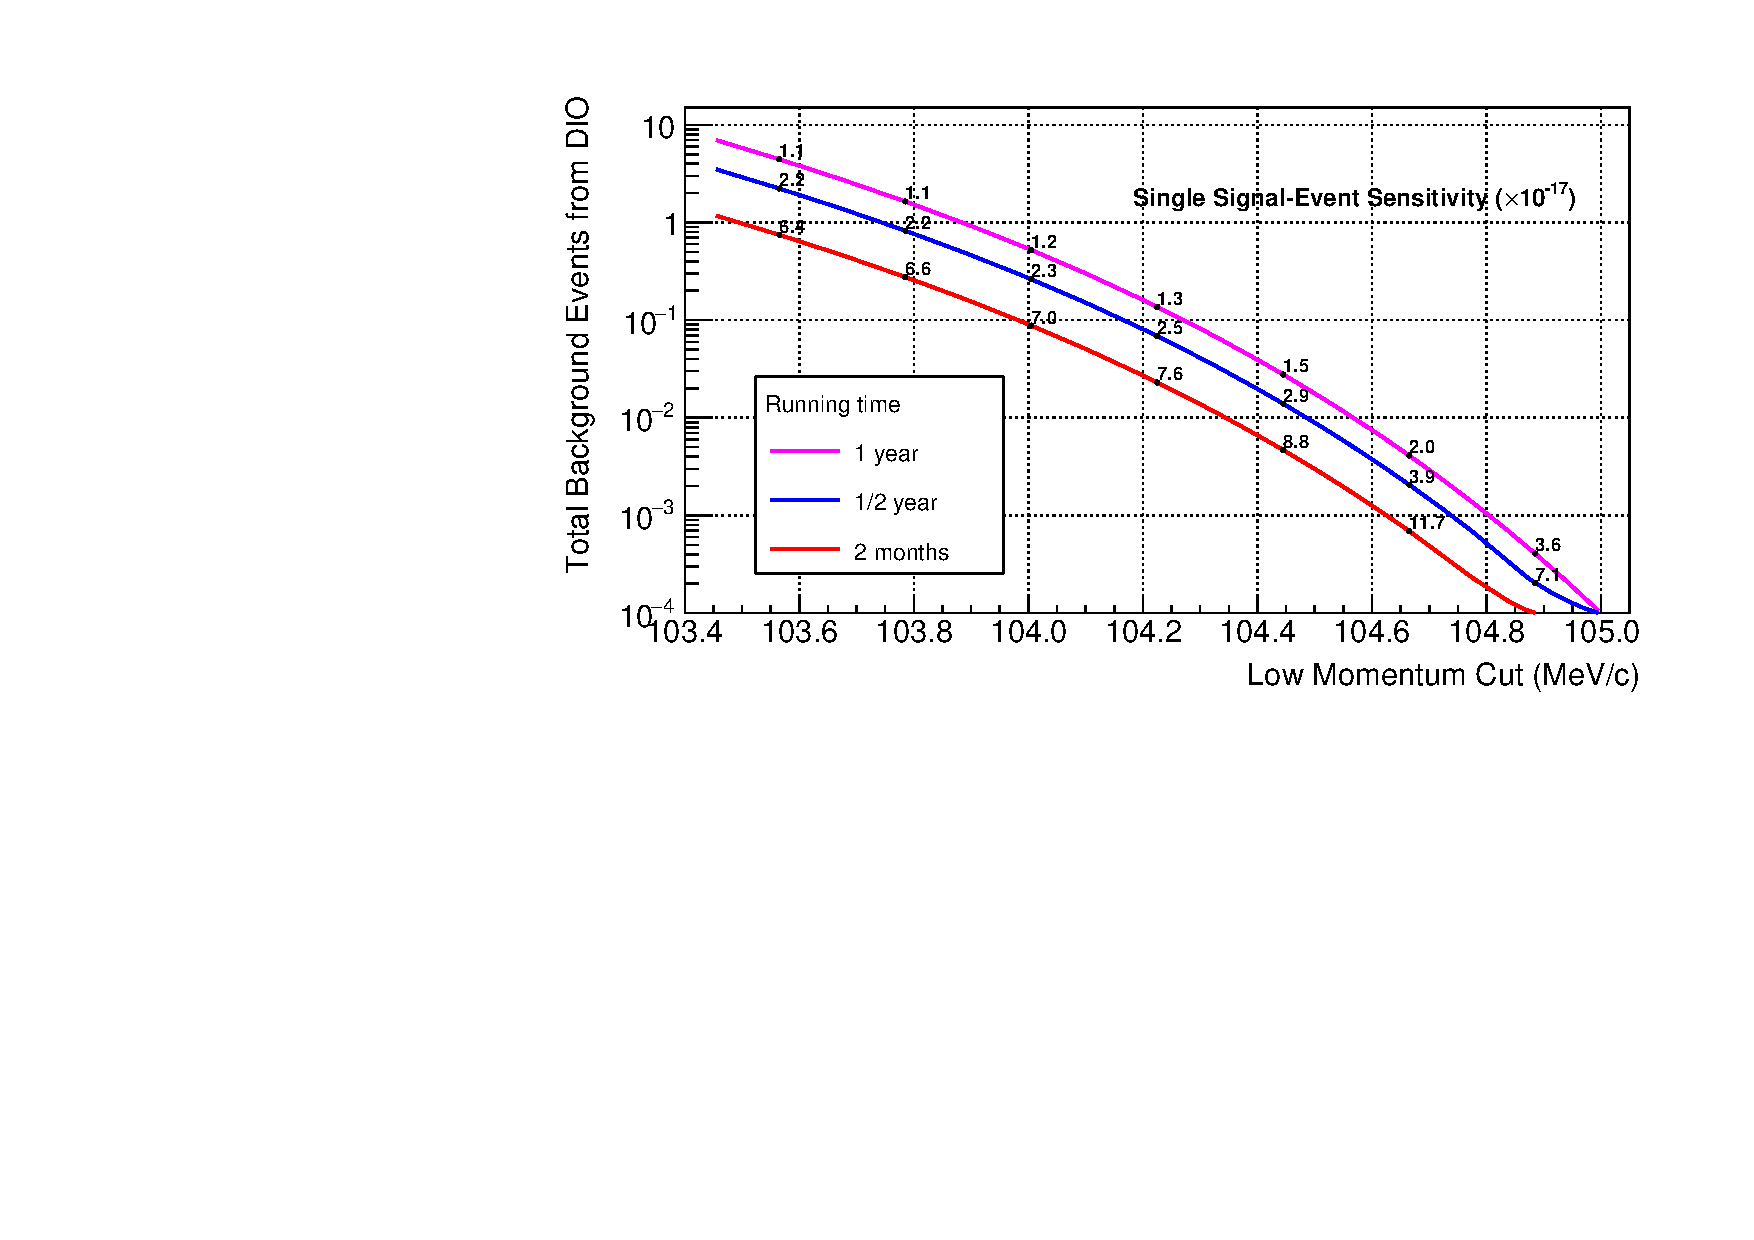
\includegraphics[width=1.0\textwidth,trim=0 0 1cm 0.93cm,clip]{figs/backgrounds/Dio_BackgroundRateVsRuntime.pdf}
%}
\caption{\figlabel{bg:dio:rates}
The DIO background rate as a function of momentum threshold for different total running times.
Given a fixed the running time, the total number of stopped muons is also fixed, which in turn sets the DIO background rate for a given momentum threshold.
All signal acceptance parameters were held fixed, except for the efficiency of the momentum threshold, which when combined with the number of stopped muons determines the \ac{ses}.
The \ac{ses} is indicated in the number along the lines in units of \num{1e-17}.
}
\end{figure}
}

\newcommand{\FigDIOEndPointComparison}{
\begin{figure}[tbp]
\centering
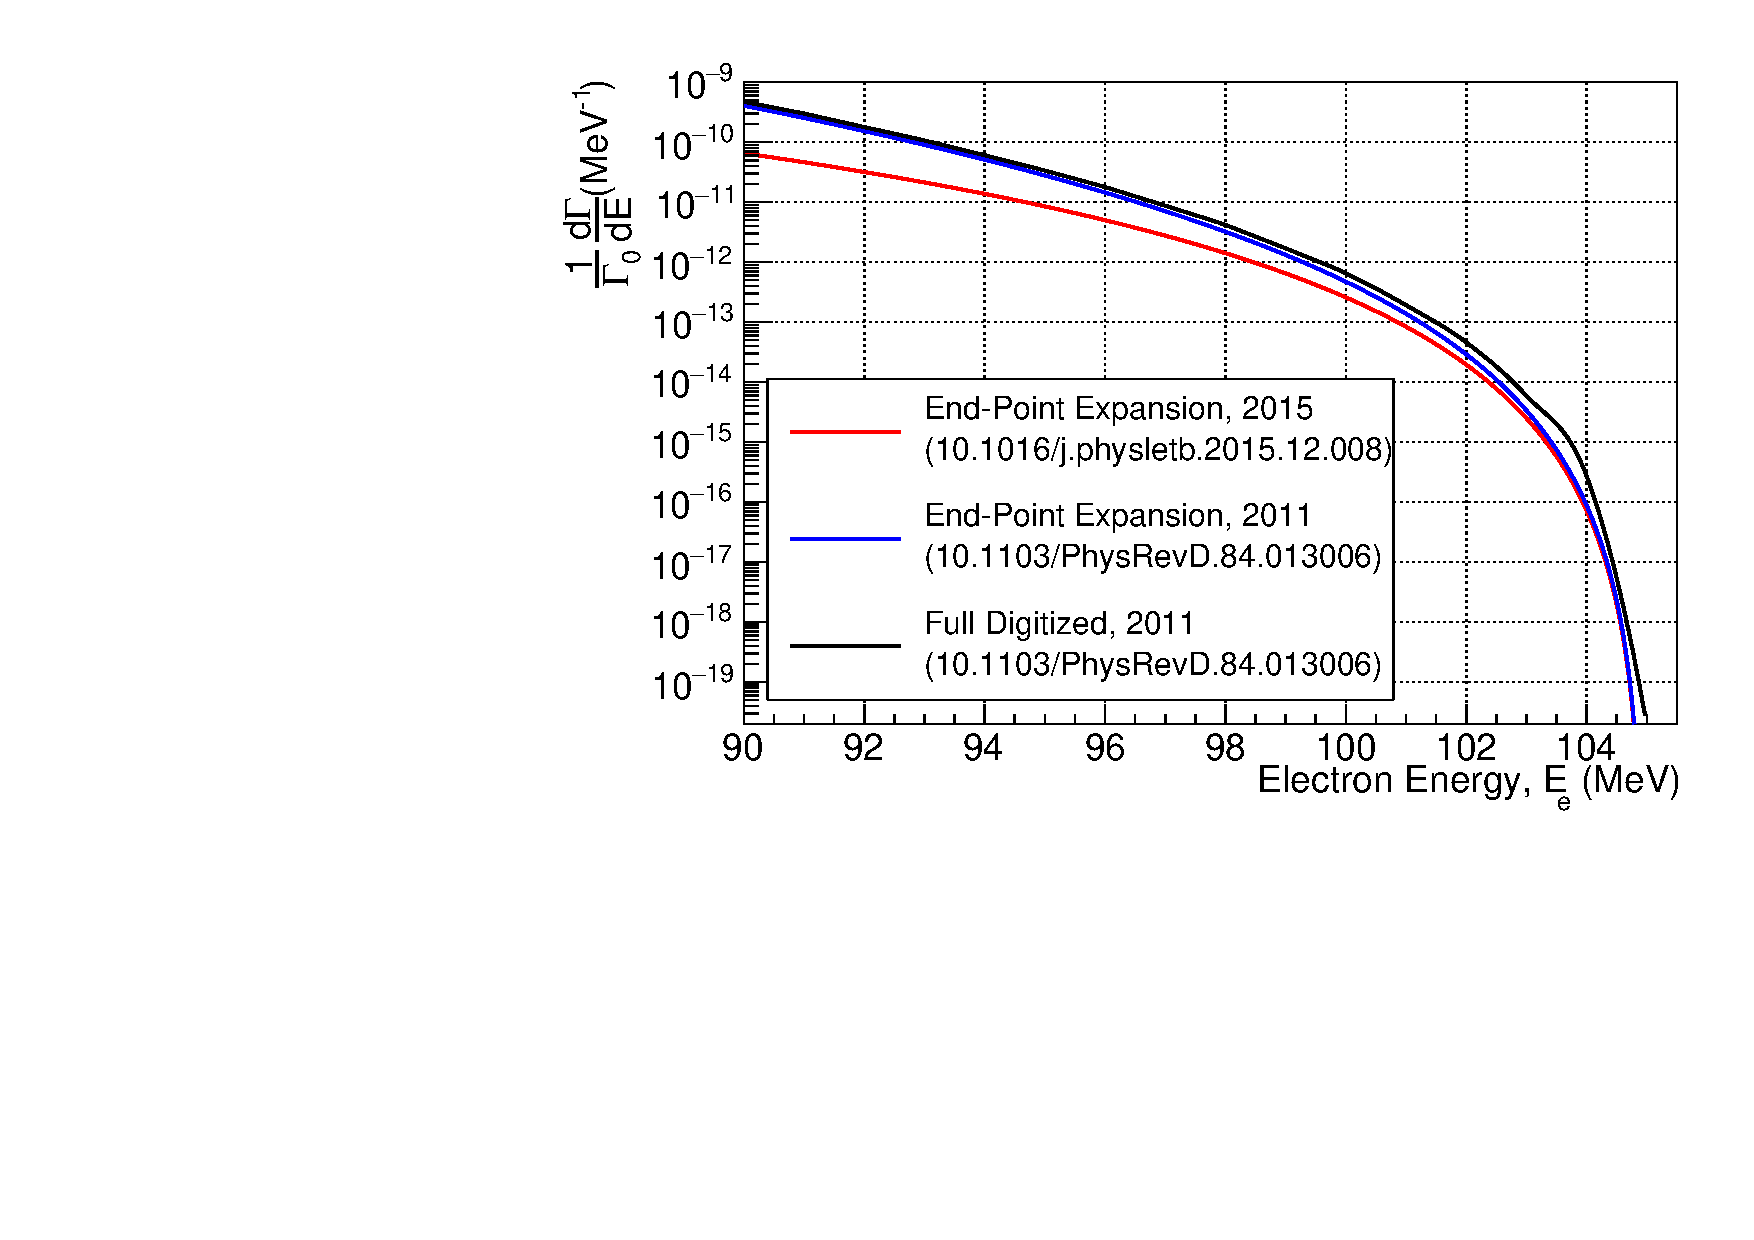
\includegraphics[width=0.8\textwidth,trim=0 0 0 0,clip]{figs/backgrounds/CompareDIOEndpoints.pdf}
\caption{\figlabel{bg:dio:spectra}
Comparison of the various available end-point expansions.
The red and blue lines show the parametrisations reported in the literature, whilst the black shows the digitisation of the spectrum used in SimG4.
For this study, the more conservative parametrisation from the 2011 Czarnecki paper~\cite{Czarnecki2011} has been used.
}
\end{figure}
}

\newcommand{\FigRMCExperiments}{
\begin{figure}[tbp]
\centering
%\fbox{
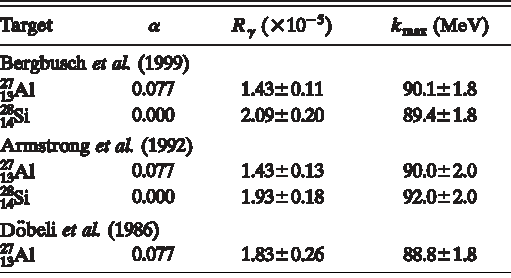
\includegraphics[width=0.5\textwidth]{figs/backgrounds/RMC_Gorringe_ExperimentSummary.pdf}
%}
\caption{\figlabel{bg:rmc:experiments}
Summary of experimental values of the rate of \ac{RMC} producing photons with energy grater than 57~MeV, and the observed end-point, reproduced from~\cite{RevModPhys.76.31}.
The column lablled `$\alpha$' is the neutron excess for the element, determined by: $\alpha=(A-2Z)/Z$.
}
\end{figure}
}

\newcommand{\TabRMCEndPoints}{%
\begin{table}[tb]%
%\centering
\begin{tabular}{lSSS}%
\hline
Reaction & \multicolumn{1}{m{3cm}}{Atomic Mass of Daughter (u)} & \multicolumn{1}{m{2cm}}{$\Delta{}M$ (MeV/c$^{2}$)}&  \multicolumn{1}{m{2cm}}{$\max(E_e^\textrm{RMC})$ (MeV/c$^{2}$)} \\
\hline
${}^{27}$Al$(\mu,\gamma\nu){}^{27}  $Mg     & 26.984341 &  3.12  & 101.85 \\
${}^{27}$Al$(\mu,\gamma\nu2n){}^{26}$Mg     & 25.982593 &  9.56  &  95.41 \\
${}^{27}$Al$(\mu,\gamma\nu2n){}^{25}$Mg     & 24.985837 & 20.66  &  84.31 \\
${}^{27}$Al$(\mu,\gamma\nu{}p){}^{26}$Na    & 25.992633 & 18.13  &  87.37 \\
${}^{27}$Al$(\mu,\gamma\nu{}np){}^{25}$Na   & 24.989954 & 23.71  &  81.77 \\
${}^{27}$Al$(\mu,\gamma\nu{}d){}^{25}$Na    & 24.989954 & 21.49  &  84.00 \\
${}^{27}$Al$(\mu,\gamma\nu\alpha){}^{23}$Na & 22.994467 & 15.49  &  91.01 \\
\hline
\end{tabular}
\caption{\tablabel{bg:rmc:massDifferences}%
Several potential daughter nuclei of nuclear muon capture in \textsuperscript{27}Al.
The mass of \textsuperscript{27}Al is 26.98153863~$u$, and one $u$ is taken as 931.494061~MeV/c$^2$~\cite{PDG2014}.
All masses come from~\cite{AUDI20033}.}\end{table}%
\xspace}%

\newcommand{\FigRMCSimResults}{
\begin{figure}[tbp]
\centering
%\fbox{
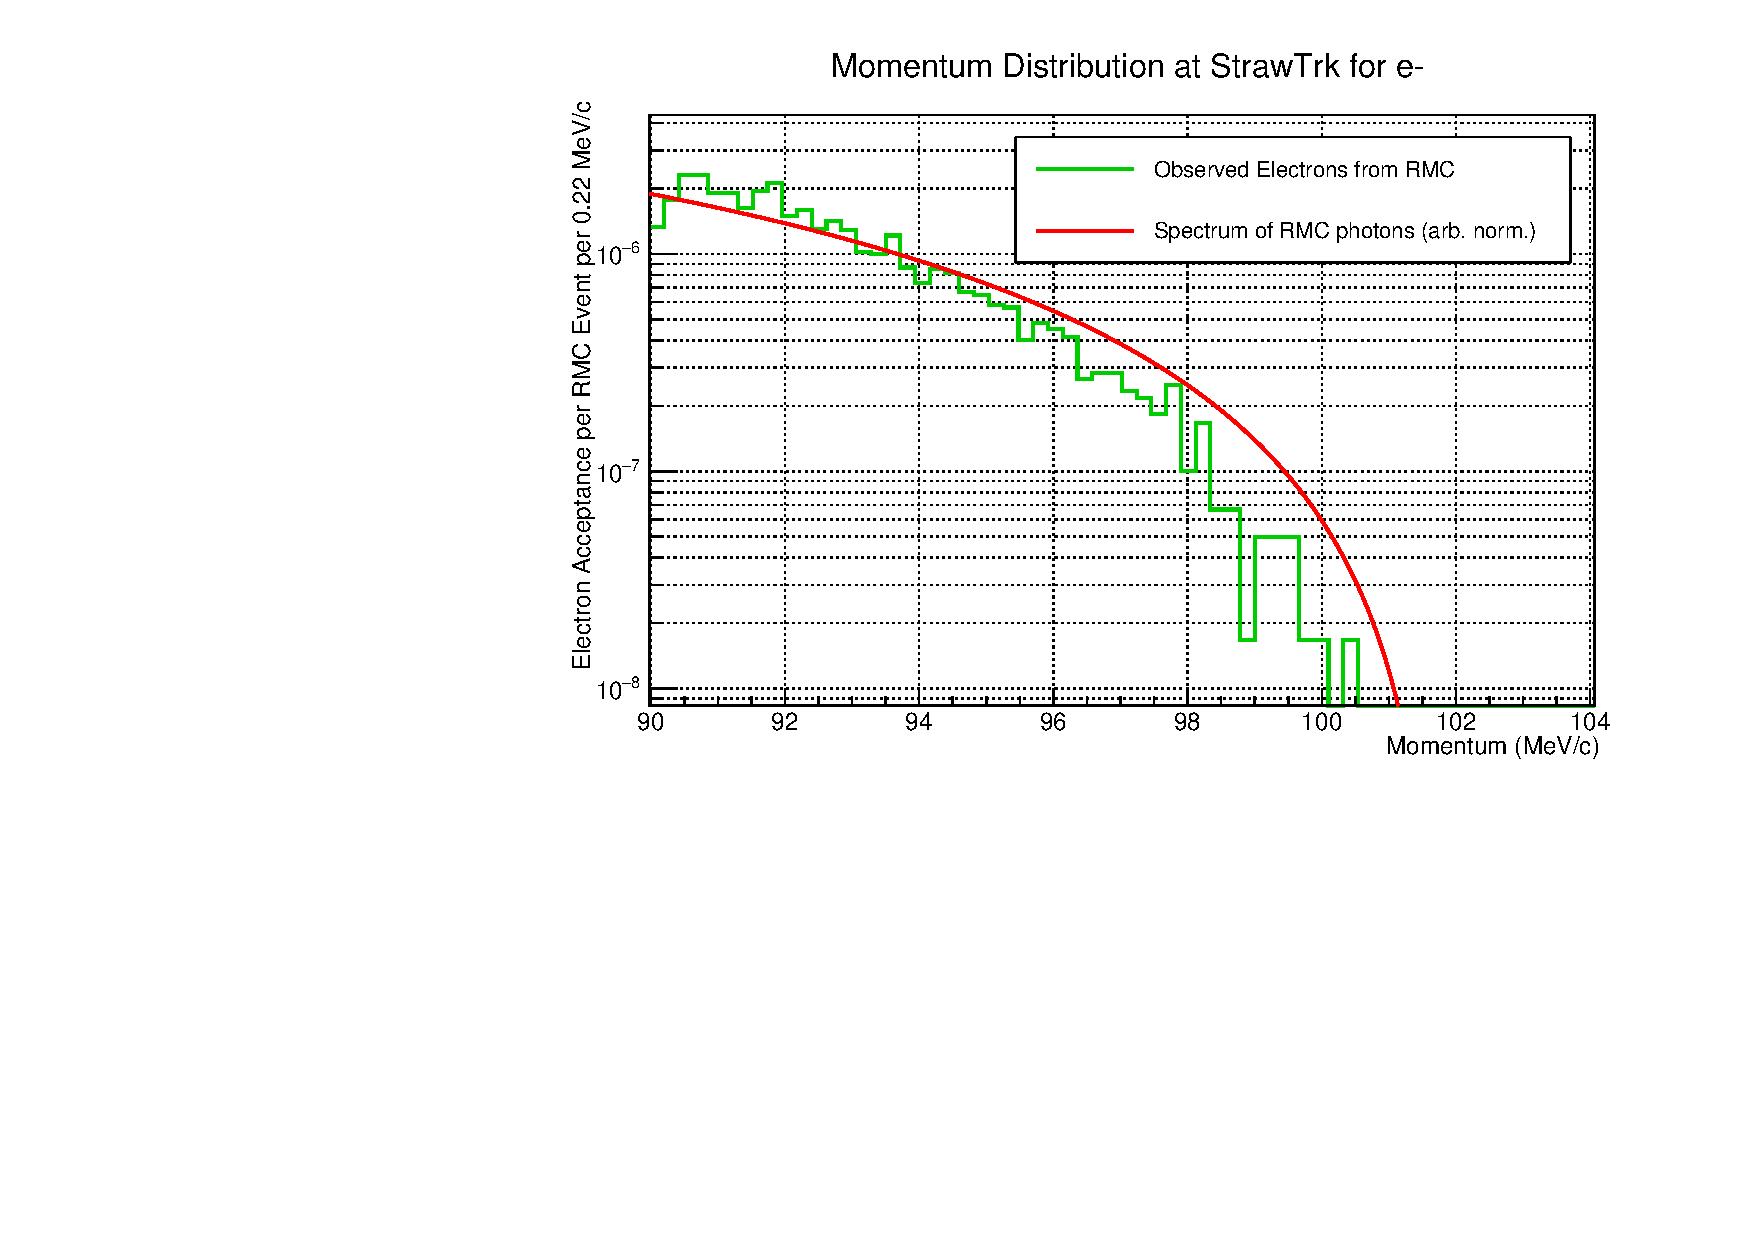
\includegraphics[width=0.85\textwidth]{figs/backgrounds/RMC_simResults.pdf}
%}
\caption{\figlabel{bg:rmc:simulation}
Observed electrons from a simulation of \num{6e7} \ac{RMC} photons.
The overlaid spectrum is normalised arbitrarily to fit on the plot.
}
\end{figure}
}

\newcommand{\FigRPCData}{
\begin{figure}[btp]
\centering
\subfloat[][\figlabel{bg:rpc:data:ca}Calcium]  {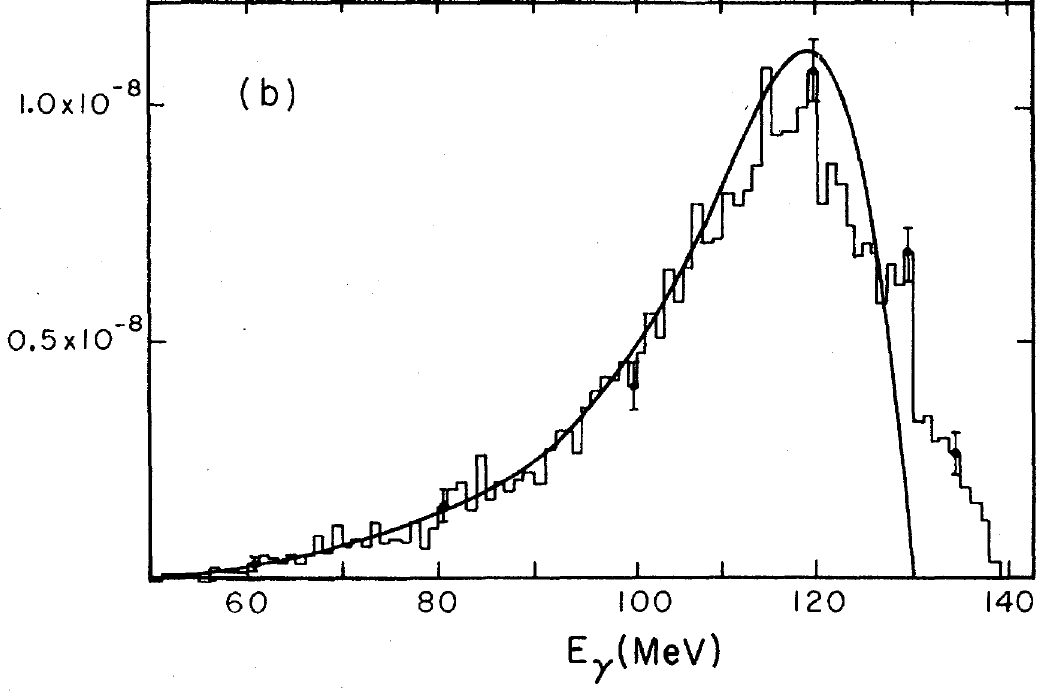
\includegraphics[width=0.43\textwidth]{figs/backgrounds/RPC-data-calcium.png}}\hspace{0.2cm}%
\subfloat[][\figlabel{bg:rpc:data:mg}Magnesium]{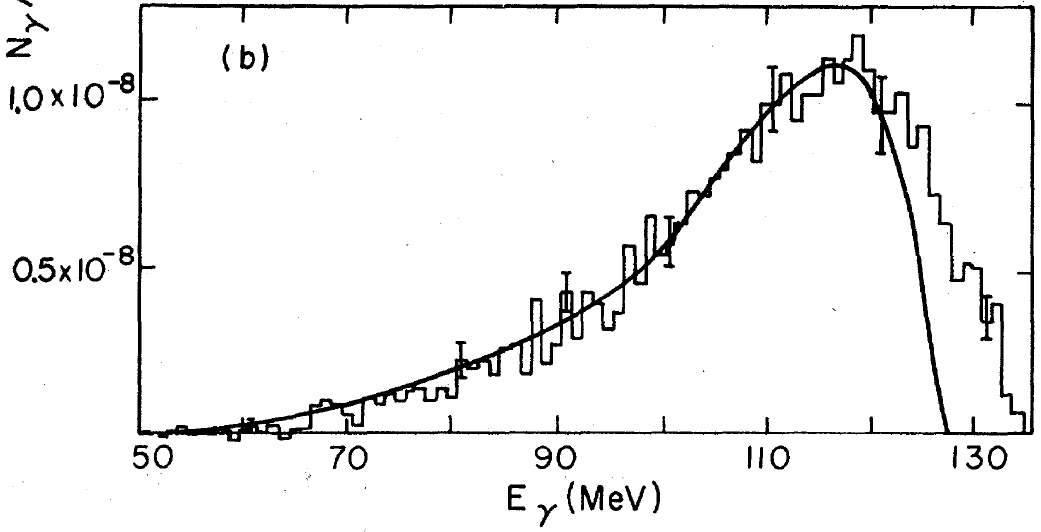
\includegraphics[width=0.53\textwidth]{figs/backgrounds/RPC-data-magnesium.png}}
\caption{\figlabel{bg:rpc:data}
Spectrum of photons coming from \acf{RPC}~\cite{Bistirlich:1972jy}.
The spectrum of manesium, which is adjacent to aluminium on the periodic table, was used as the basis of these studies.
}
\end{figure}
}

\newcommand{\FigRPCSimulatedSpectrum}{
\begin{figure}[btp]
\centering
%\fbox{%
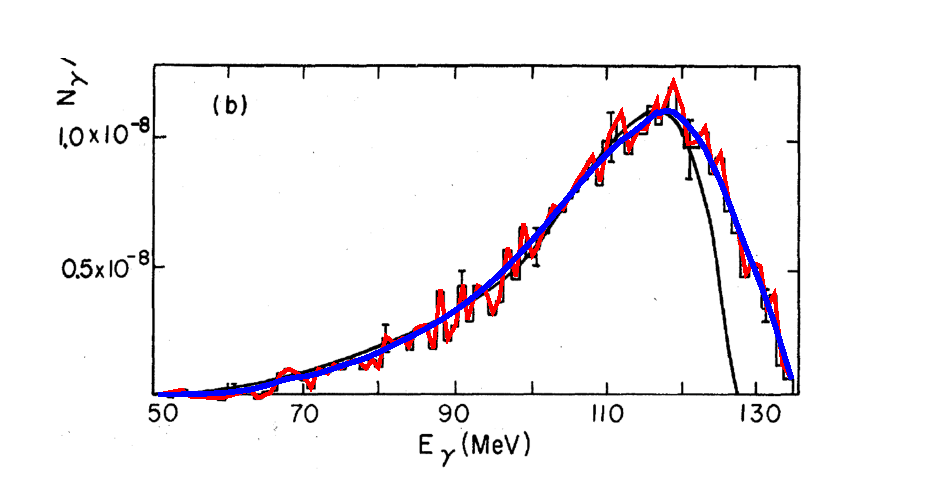
\includegraphics[width=0.73\textwidth,trim=1cm 0.5cm 2cm 1cm,clip]{figs/backgrounds/RPC_simulated_spectrum.pdf}%
%}
\caption{\figlabel{bg:rpc:spectrum}
Digitised (red) and smoothed (blue) spectrum of \ac{RPC} from magnesium (see \fig{bg:rpc:data:mg}) used as input to the Monte Carlo simulation.
}
\end{figure}
}

\newcommand{\FigPionStopDist}{
\begin{figure}[btp]
\centering
\subfloat[][\figlabel{bg:piStop:dist:x}X-direction]{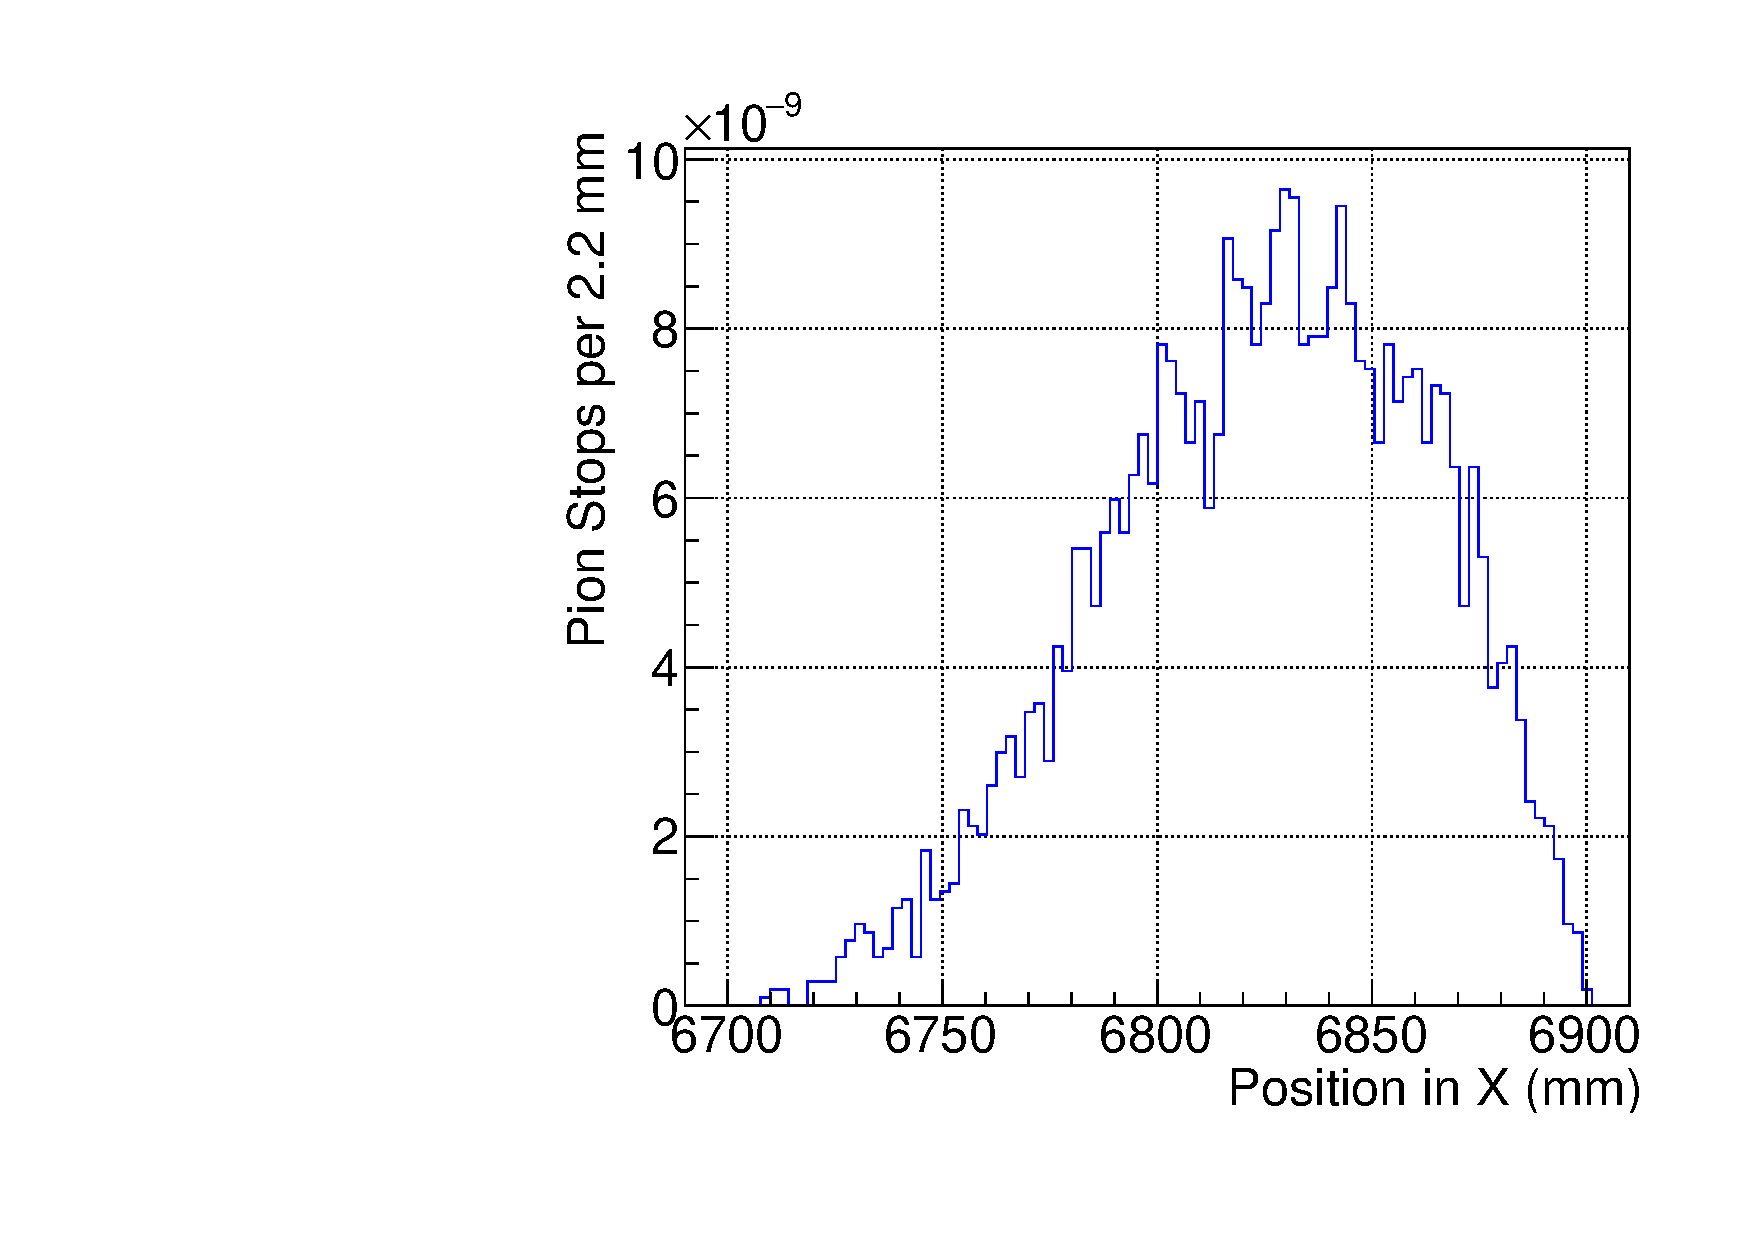
\includegraphics[width=0.32\textwidth,trim=0.2cm 0 1cm 0.7cm,clip]{figs/backgrounds/Tidied_StoppedPi-X.pdf}}\hspace{0.1cm}%
\subfloat[][\figlabel{bg:piStop:dist:y}Y-direction]{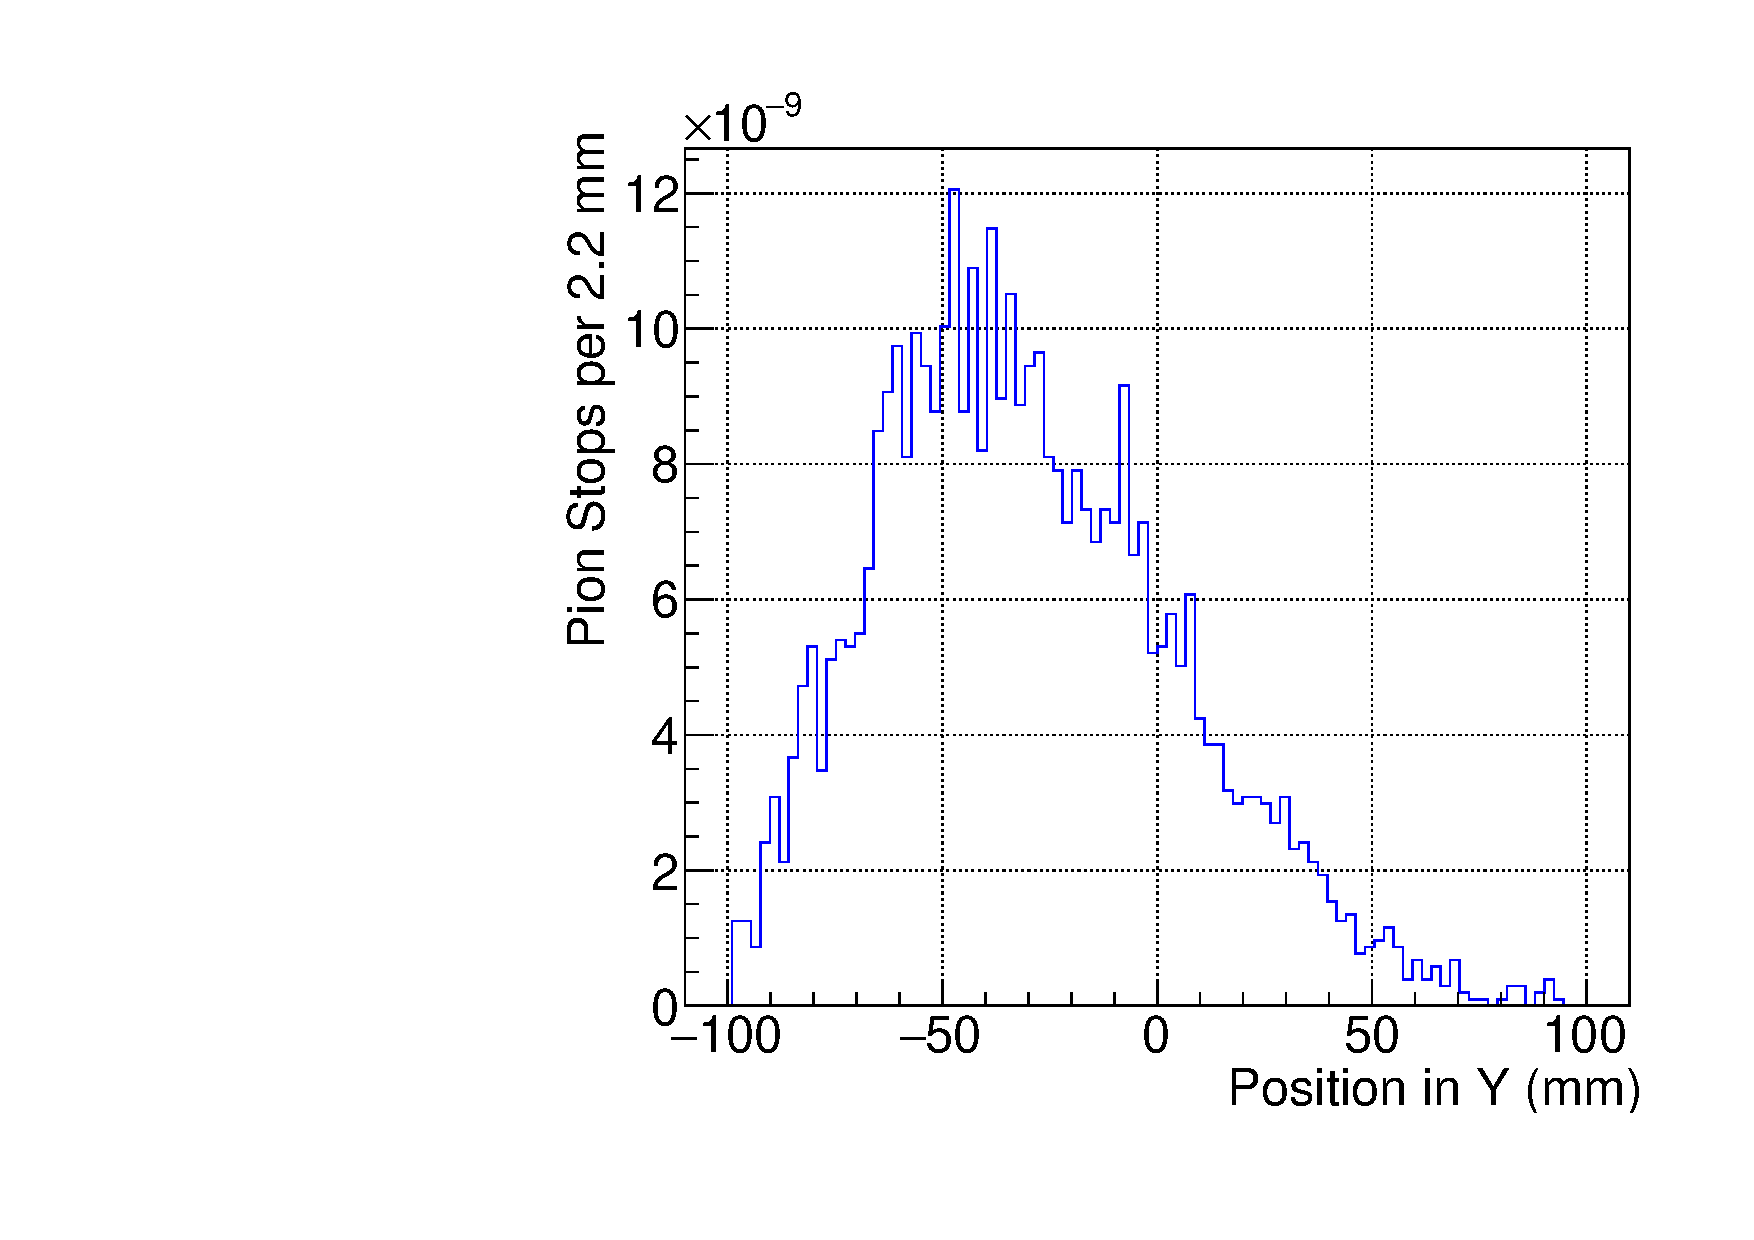
\includegraphics[width=0.32\textwidth,trim=0.2cm 0 1cm 0.7cm,clip]{figs/backgrounds/Tidied_StoppedPi-Y.pdf}}\hspace{0.1cm}%
\subfloat[][\figlabel{bg:piStop:dist:z}Z-direction]{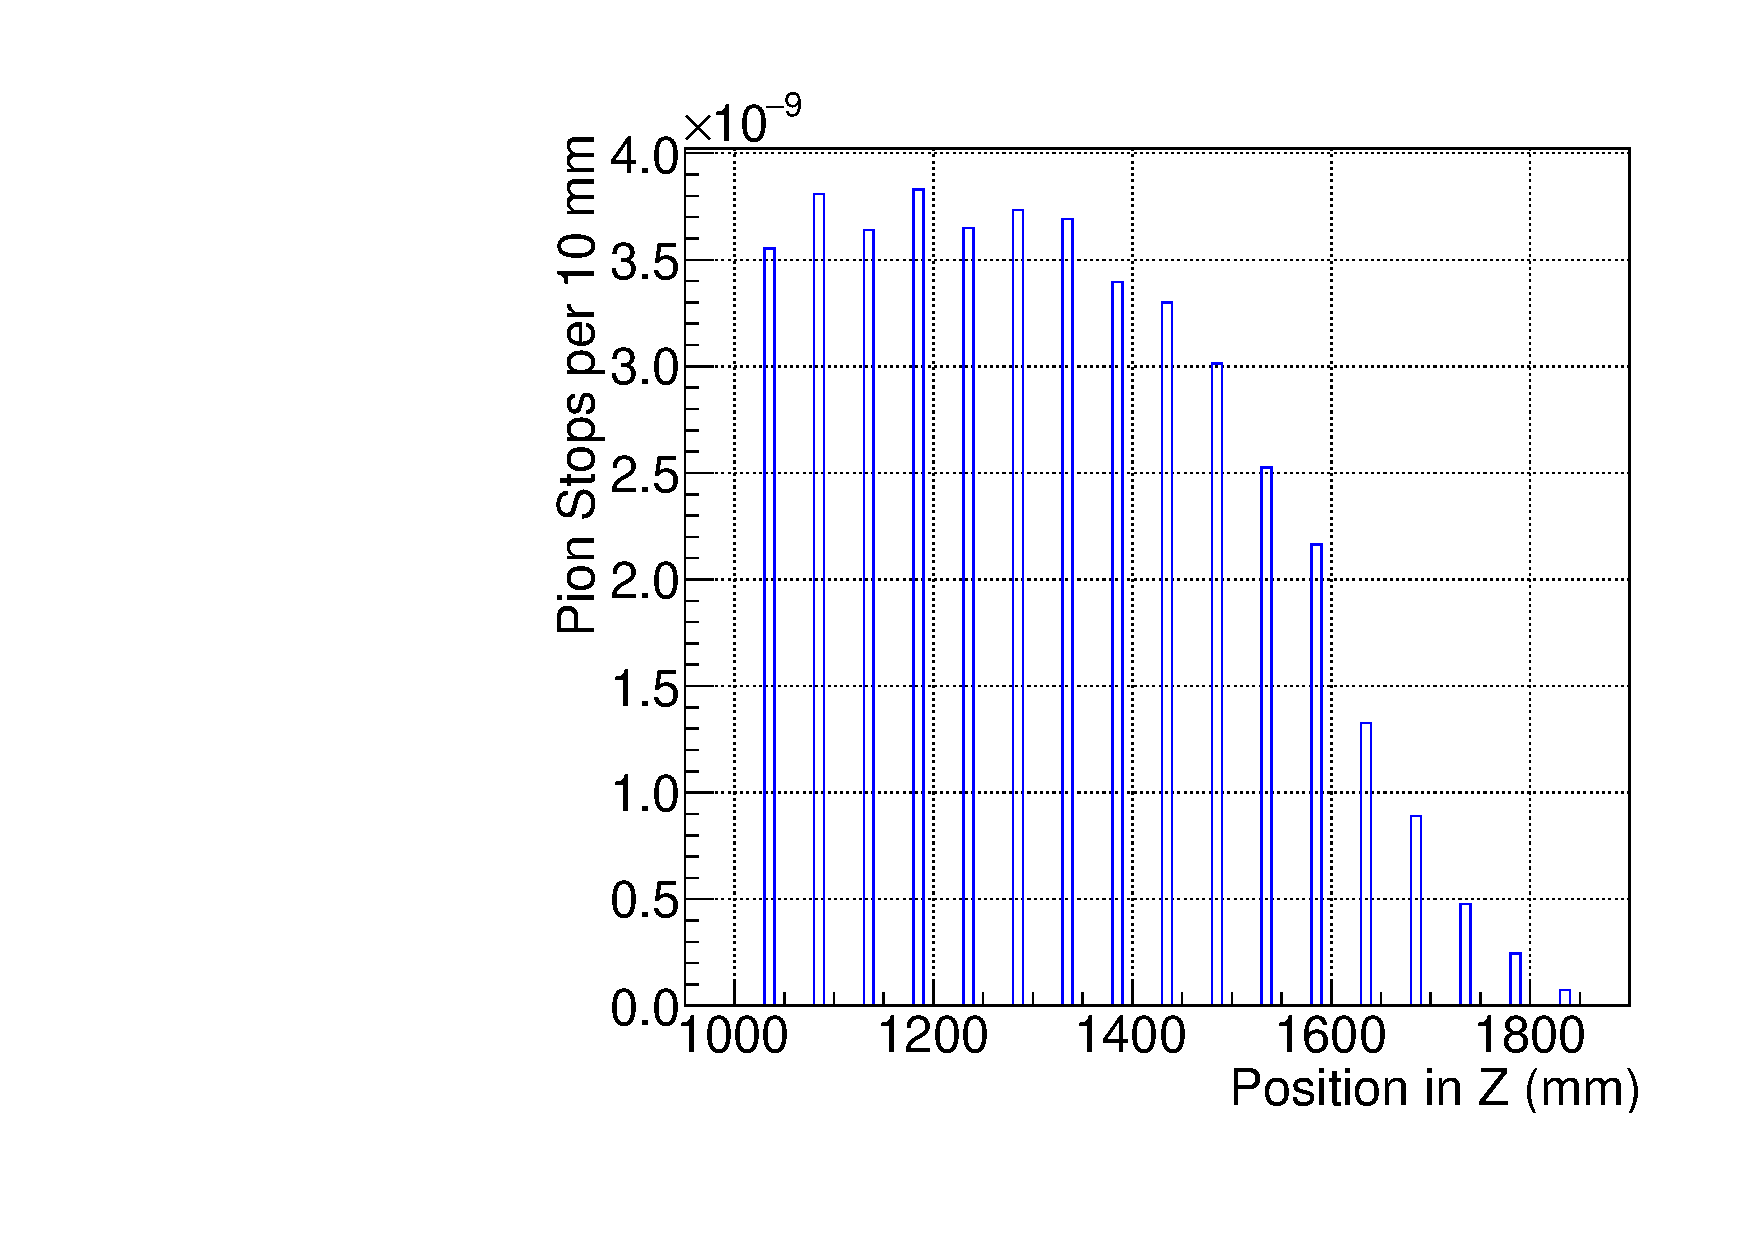
\includegraphics[width=0.32\textwidth,trim=0.2cm 0 1cm 0.7cm,clip]{figs/backgrounds/Tidied_StoppedPi-Z.pdf}}
\caption{\figlabel{bg:piStop:dist}
Stopping distributions of pions in the target.
These distributions have considerably different forms to the muon stopping distributions shown in \fig{sense:stops2D}, mostly due to the different momenta of muons and pions.
}
\end{figure}
}

\newcommand{\FigPiVsMuMomenta}{
\begin{figure}[btp]
\centering
%\fbox{%
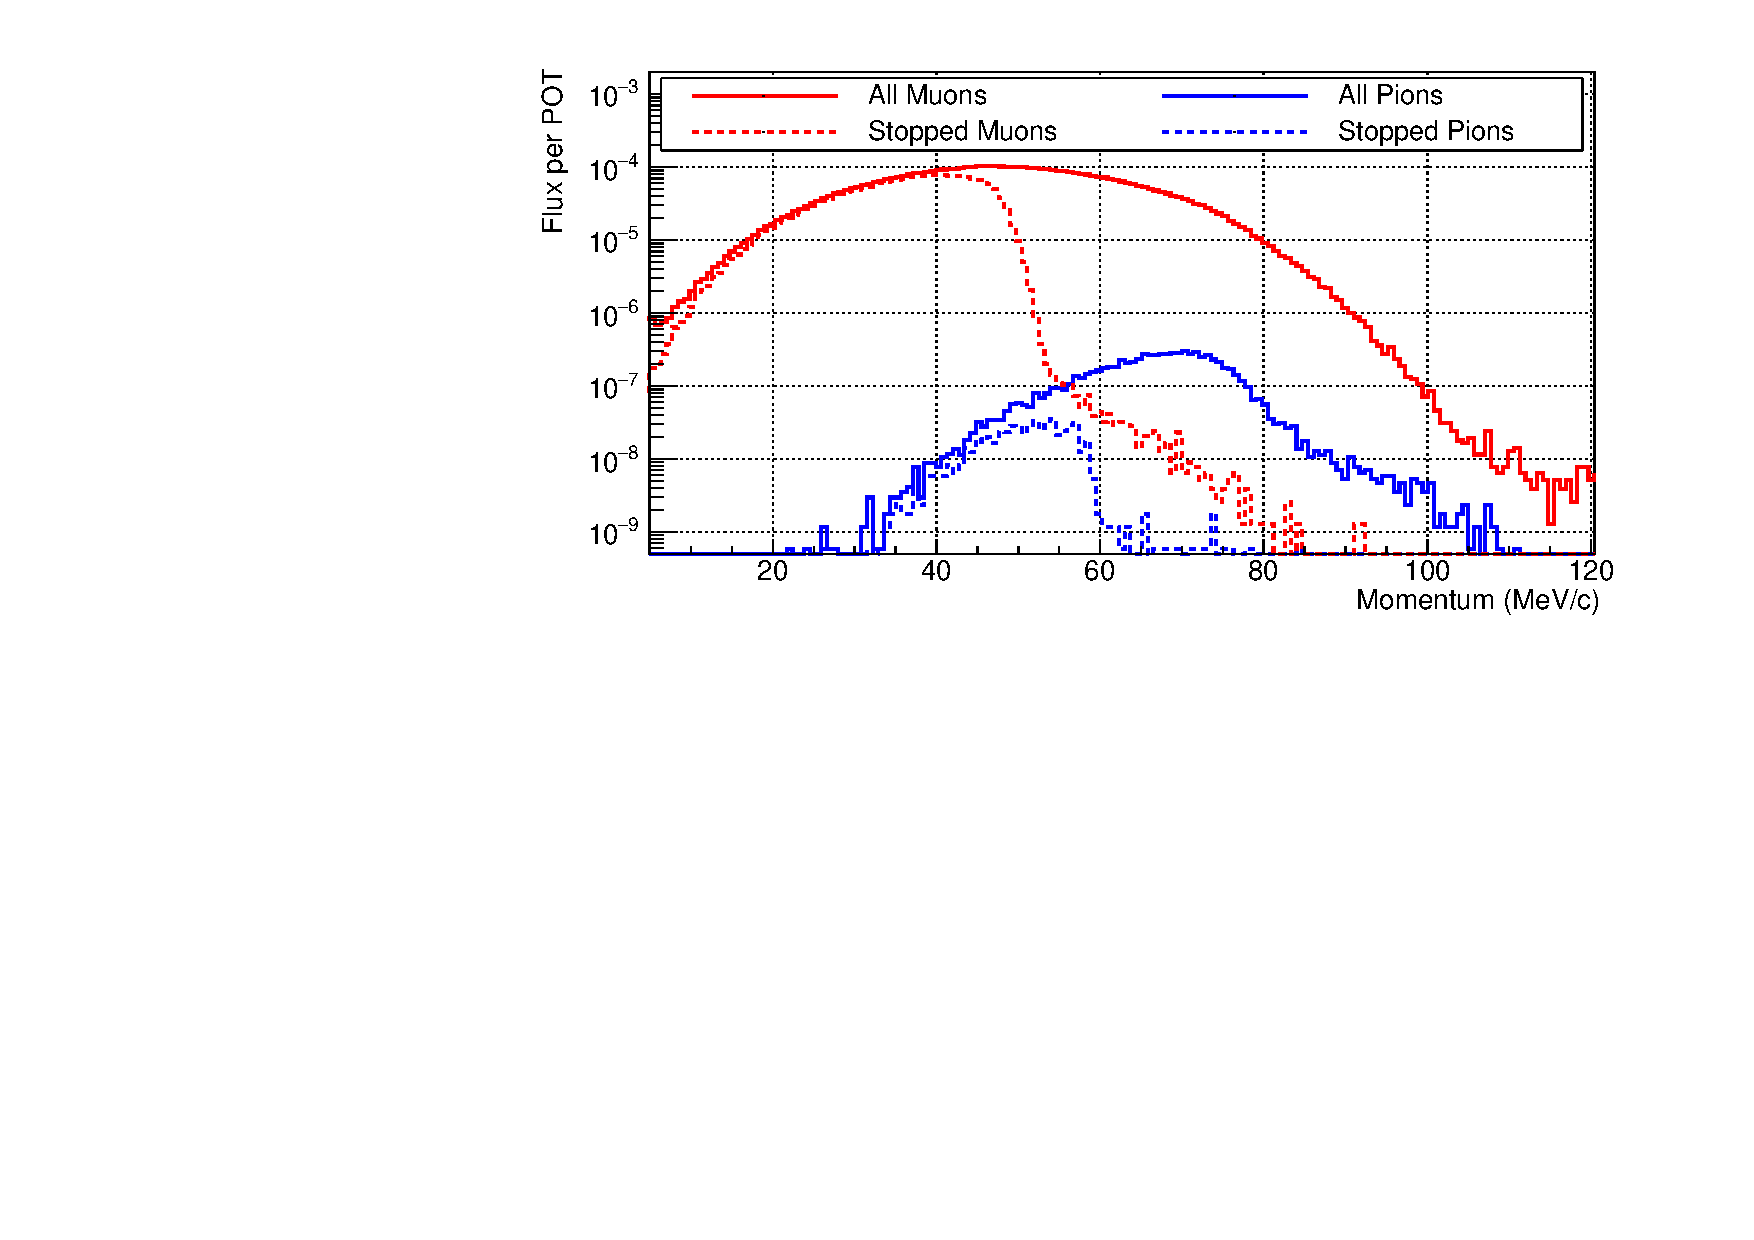
\includegraphics[width=0.9\textwidth,trim=0 0.5cm 1.3cm 0.4cm,clip]{figs/backgrounds/Tidied_MuVsPiMomentum.pdf}%
%}
\caption{\figlabel{bg:piVsMu:momenta}
The momentum of muons and pions for those that reach the target area and those that actually stop.
It is clear how the pion momenta are in general higher, including those that stop, although the maximum stopping momentum for pions is similar to that of muons.
}
\end{figure}
}

\newcommand{\FigRPCSimResults}{
\begin{figure}[btp]
\centering
\begin{minipage}[b]{0.5\textwidth}
\subfloat[][\figlabel{bg:rpc:sim:time}Arrival Time]{%
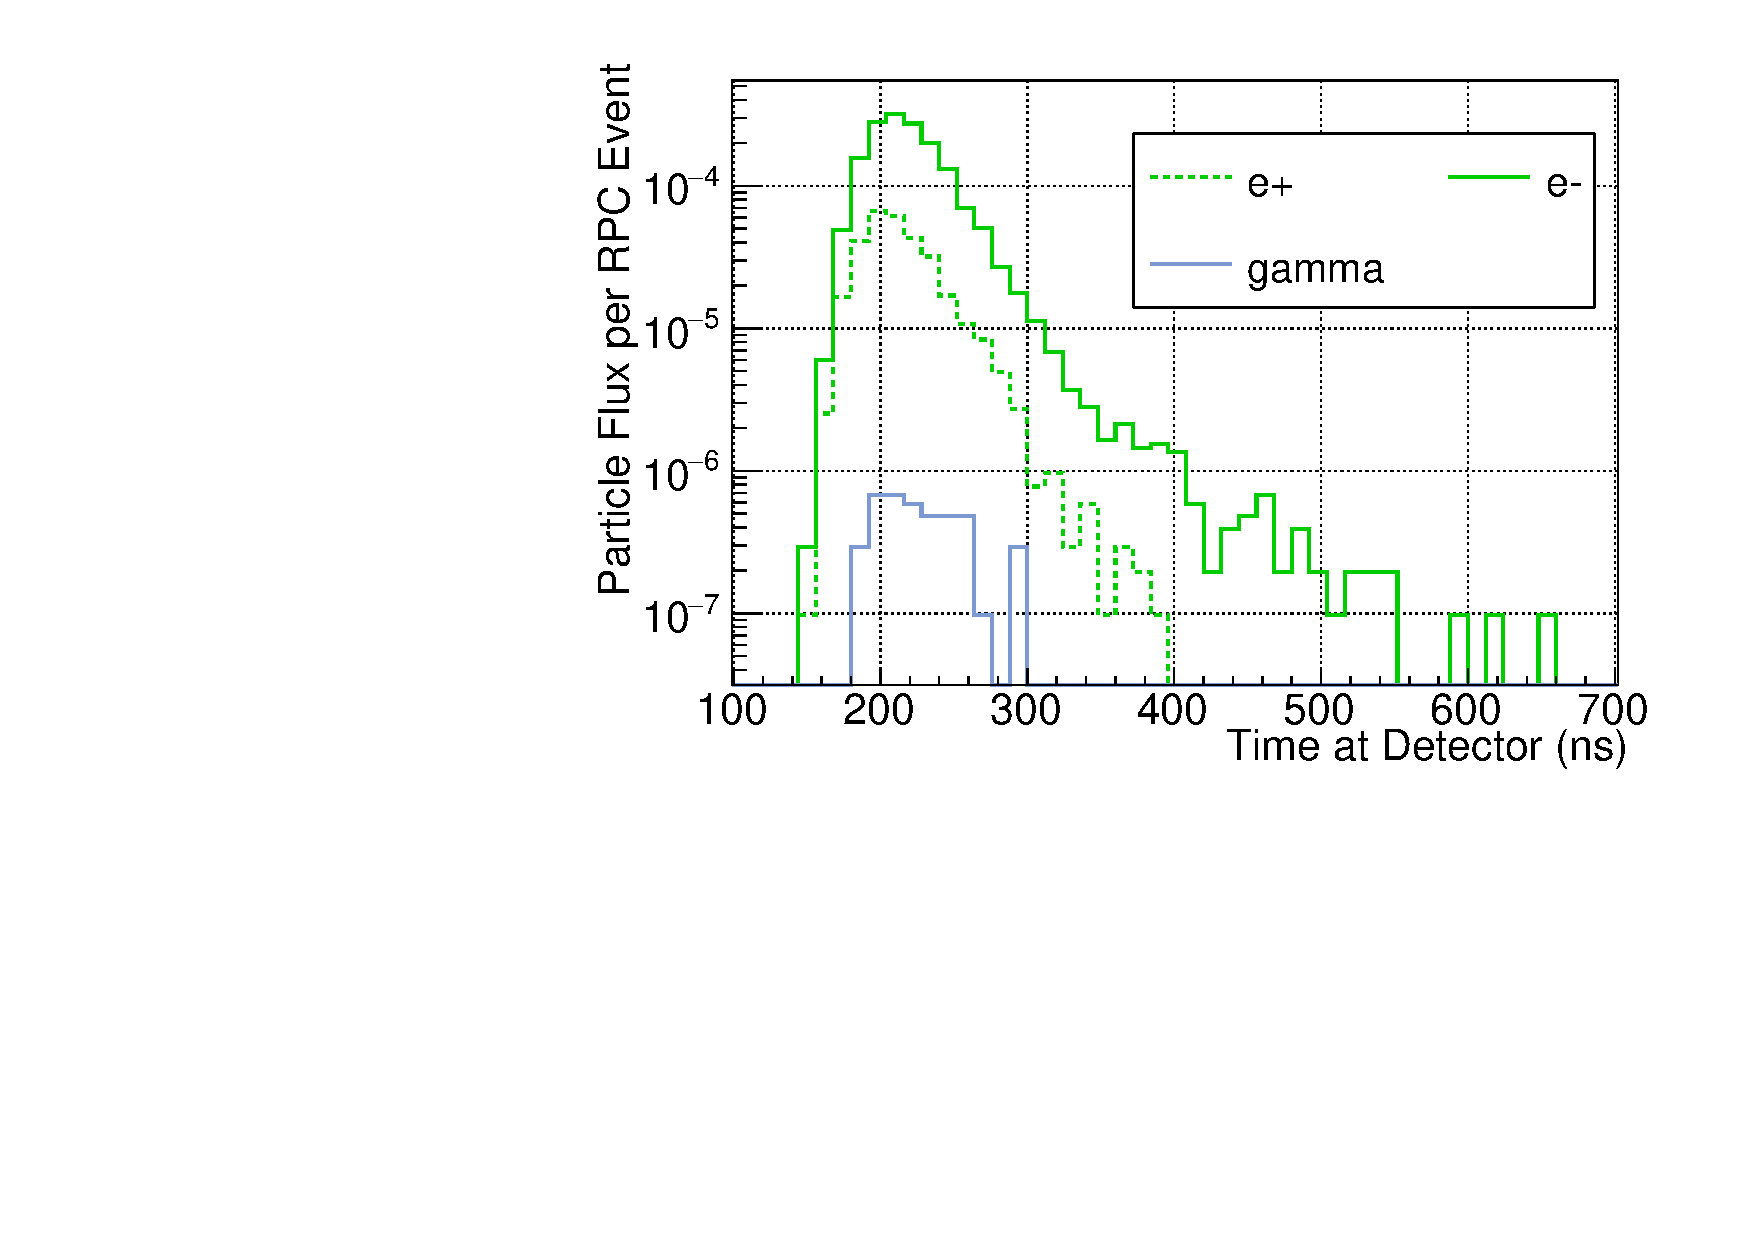
\includegraphics[width=\textwidth,trim=0.9cm 0.3cm 1cm 0.5cm,clip]{figs/backgrounds/Tidied_RPC_sim_time.pdf}}\\
\subfloat[][\figlabel{bg:rpc:sim:momVtime}Momentum Vs.\ Time]{%
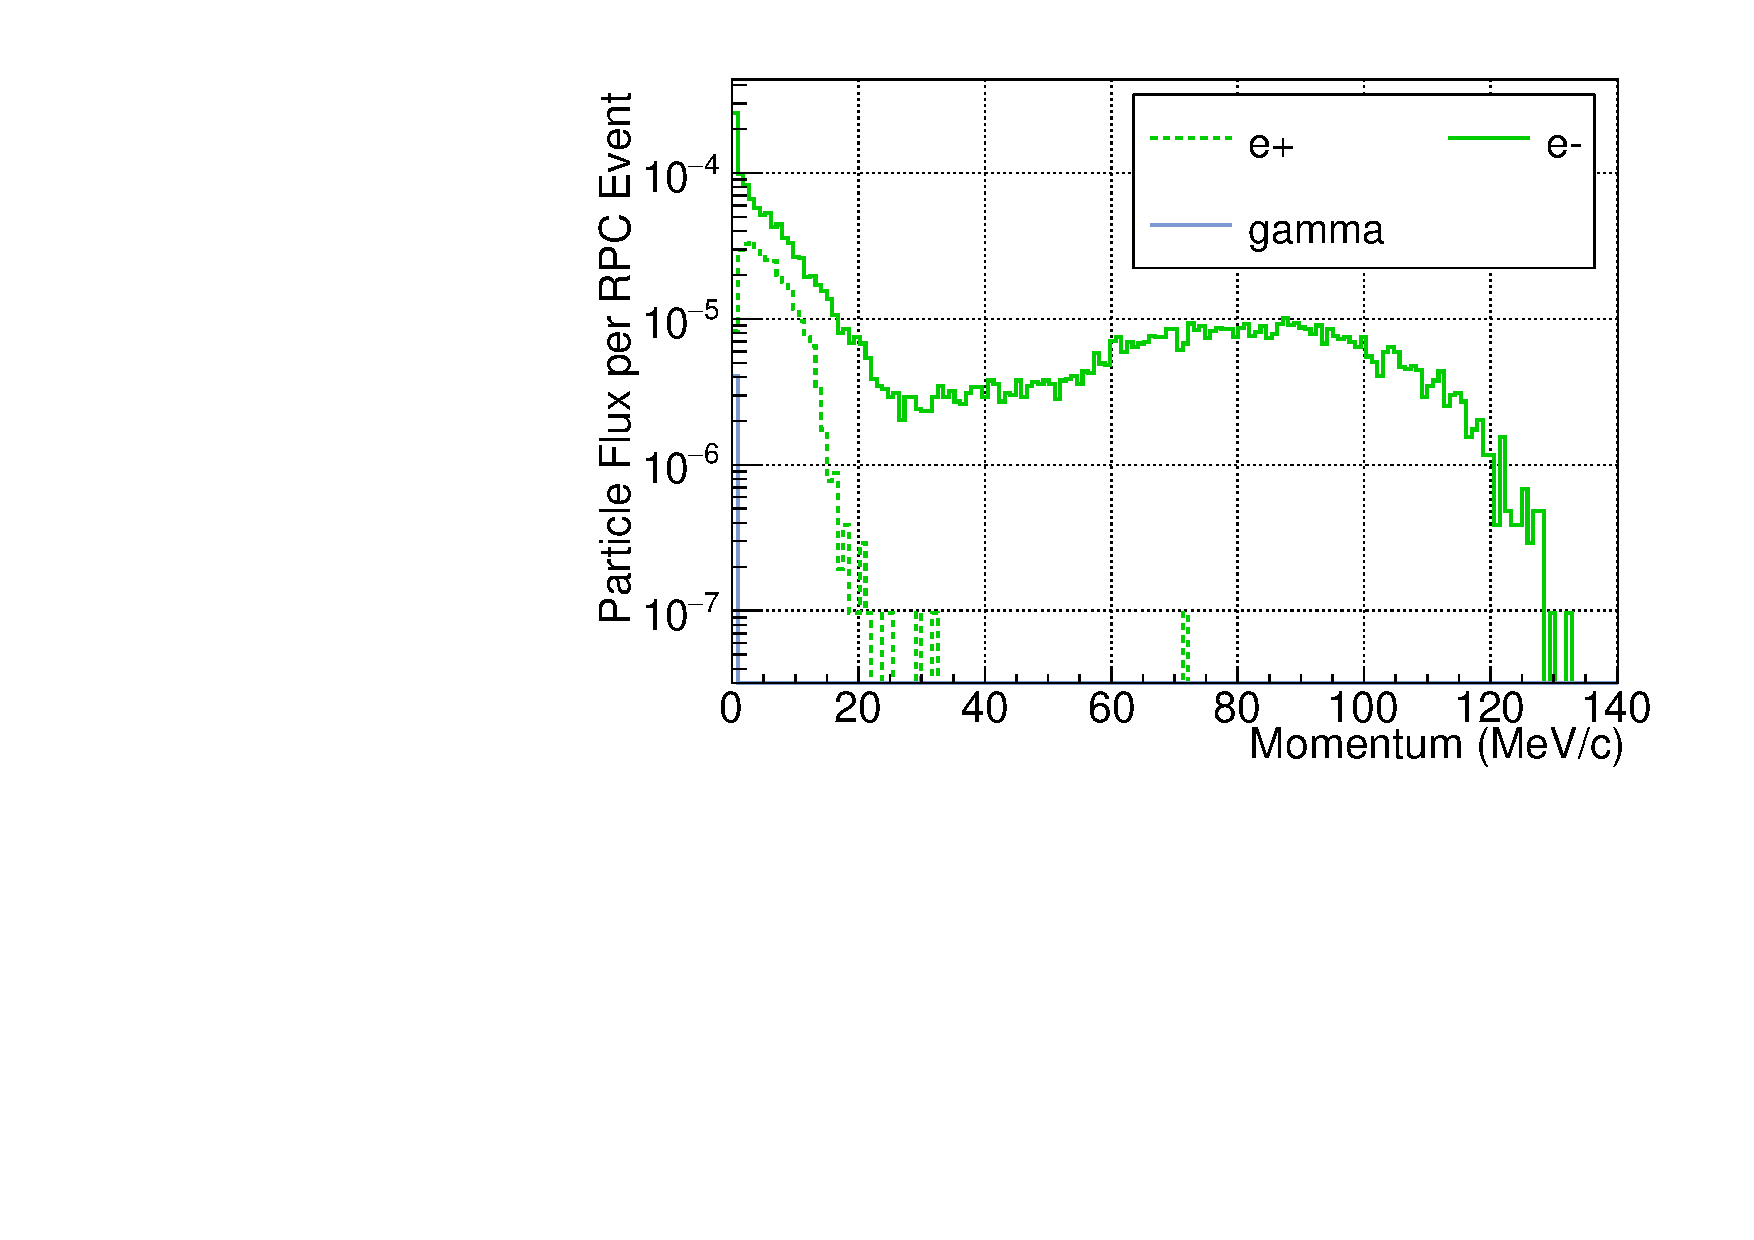
\includegraphics[width=\textwidth,trim=0.9cm 0.3cm 1cm 0.5cm,clip]{figs/backgrounds/Tidied_RPC_sim_mom.pdf}}%
\end{minipage}\hspace{1ex}
\subfloat[][\figlabel{bg:rpc:sim:mom}Momentum]{%
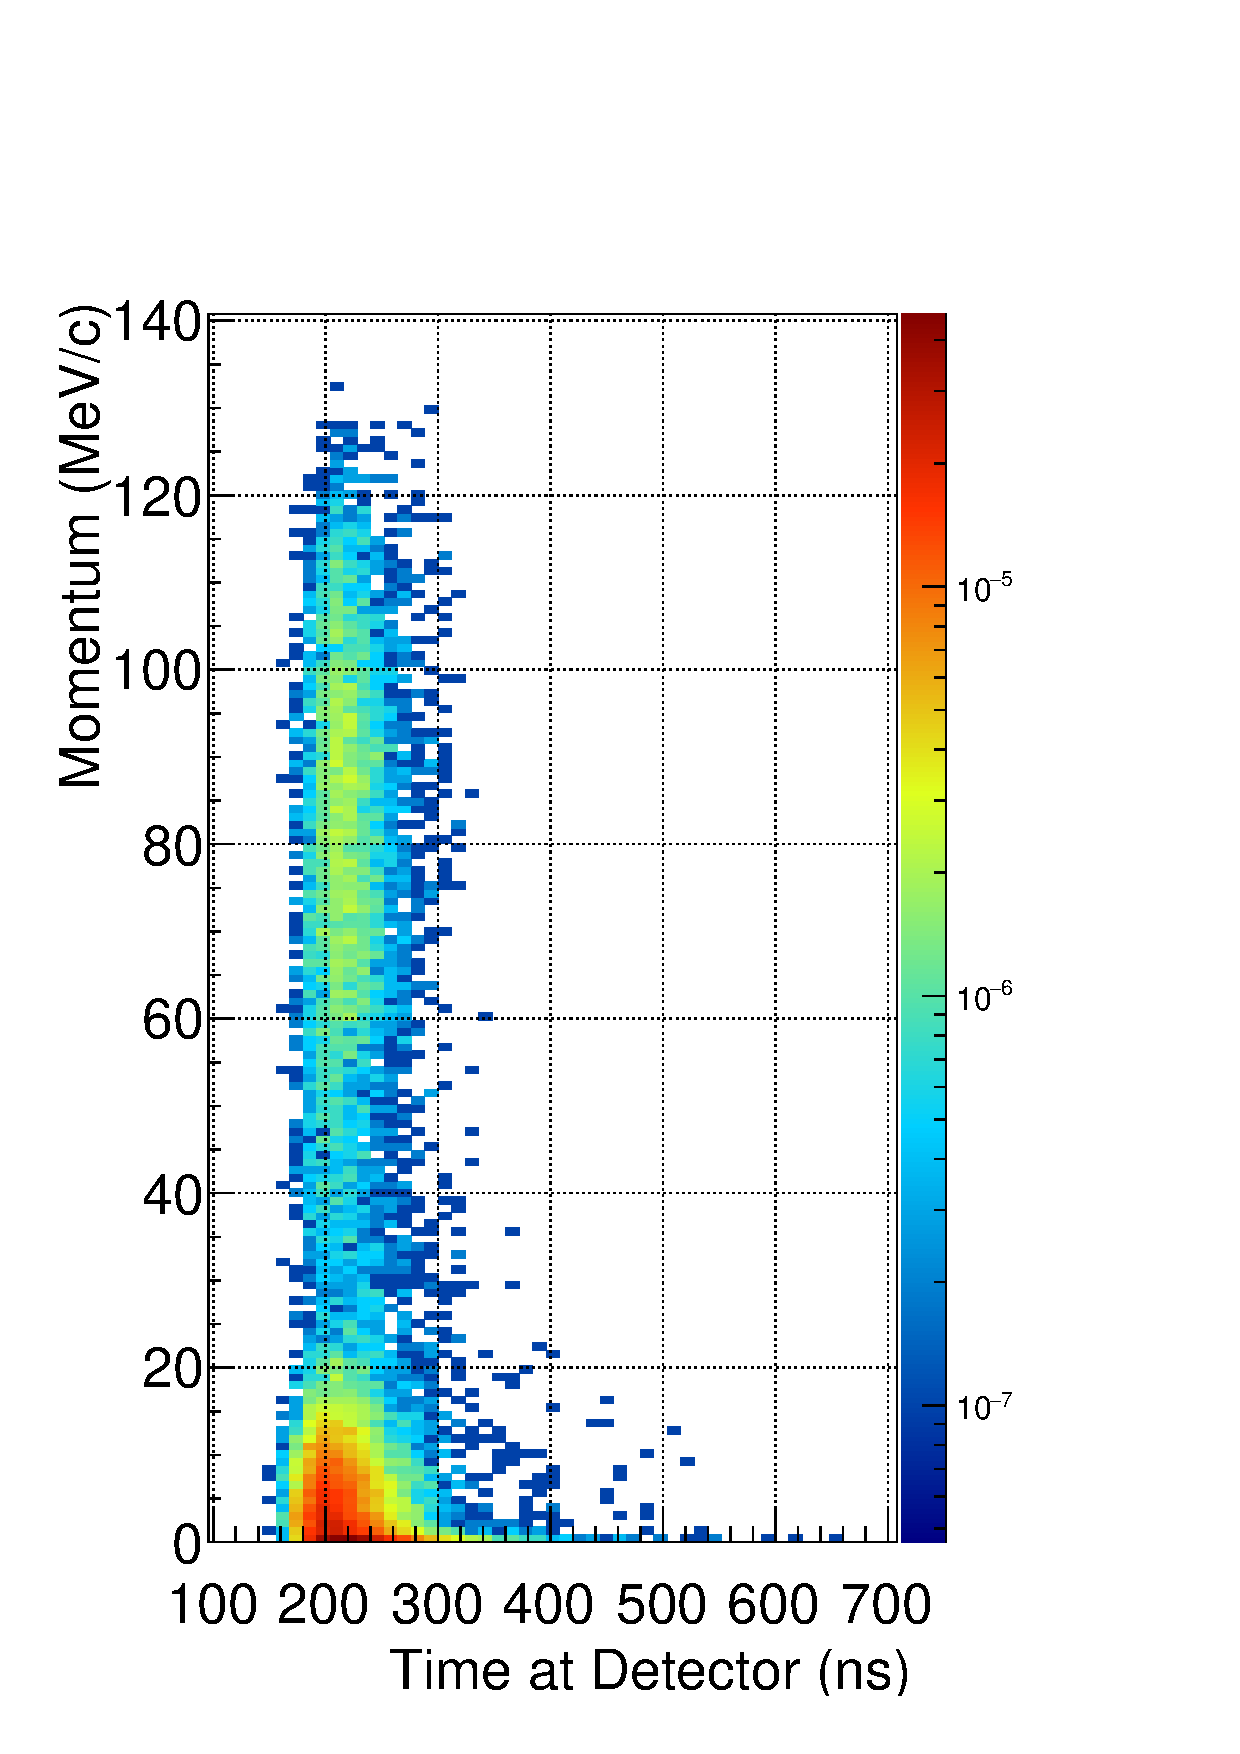
\includegraphics[width=0.45\textwidth,trim=0.2cm 0 0cm 0.7cm,clip]{figs/backgrounds/Tidied_RPC_sim_mom-time.pdf}}
\caption{\figlabel{bg:rpc:sim}
Detection of secondaries from RPC photons in the target.
Although many high-momentum electrons are detected, they are all well before the time-gated detected window.
}
\end{figure}
}

\newcommand{\FigAntiprotonData}{
\begin{figure}[tbp]
\centering
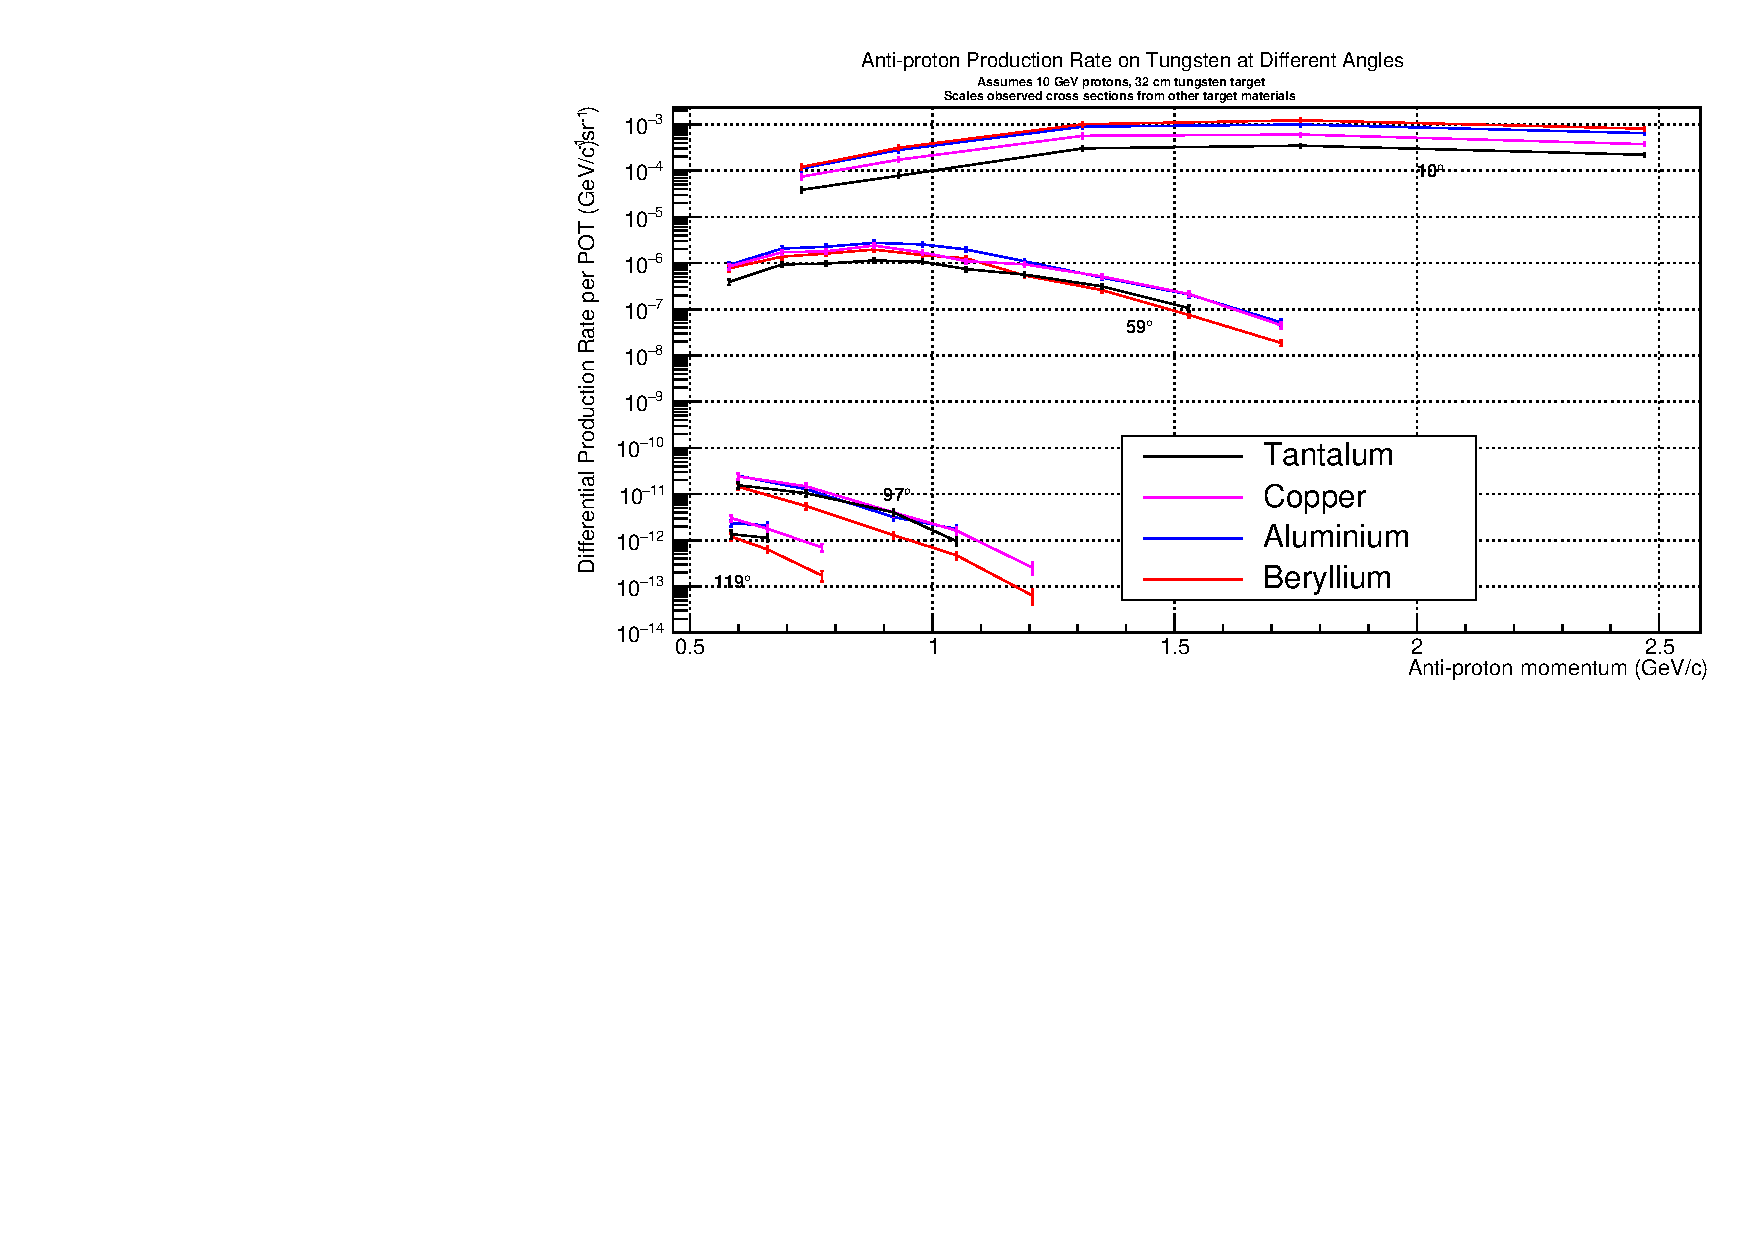
\includegraphics[width=1.0\textwidth,trim=0 0 0 0,clip]{figs/backgrounds/Antiproton_RatePerPOT_data.pdf}
\caption{\figlabel{bg:antiprotons:data}
Experimental data for antiproton production rates for 10~GeV protons~\cite{Boyarinov:1994tp,Kiselev:2012sj}.
Each line represents the cross section obtained for the four different target materials covered in those papers, scaled to match the number of nucleons of tungsten and with the additional factors of \eq{bg:antiprotons:rate} included.
}
\end{figure}
}

\newcommand{\FigAntiprotonEndpoint}{
\begin{figure}[btp]
\centering
\subfloat[][\figlabel{bg:antiprotons:end-point:tungsten}Tungsten]{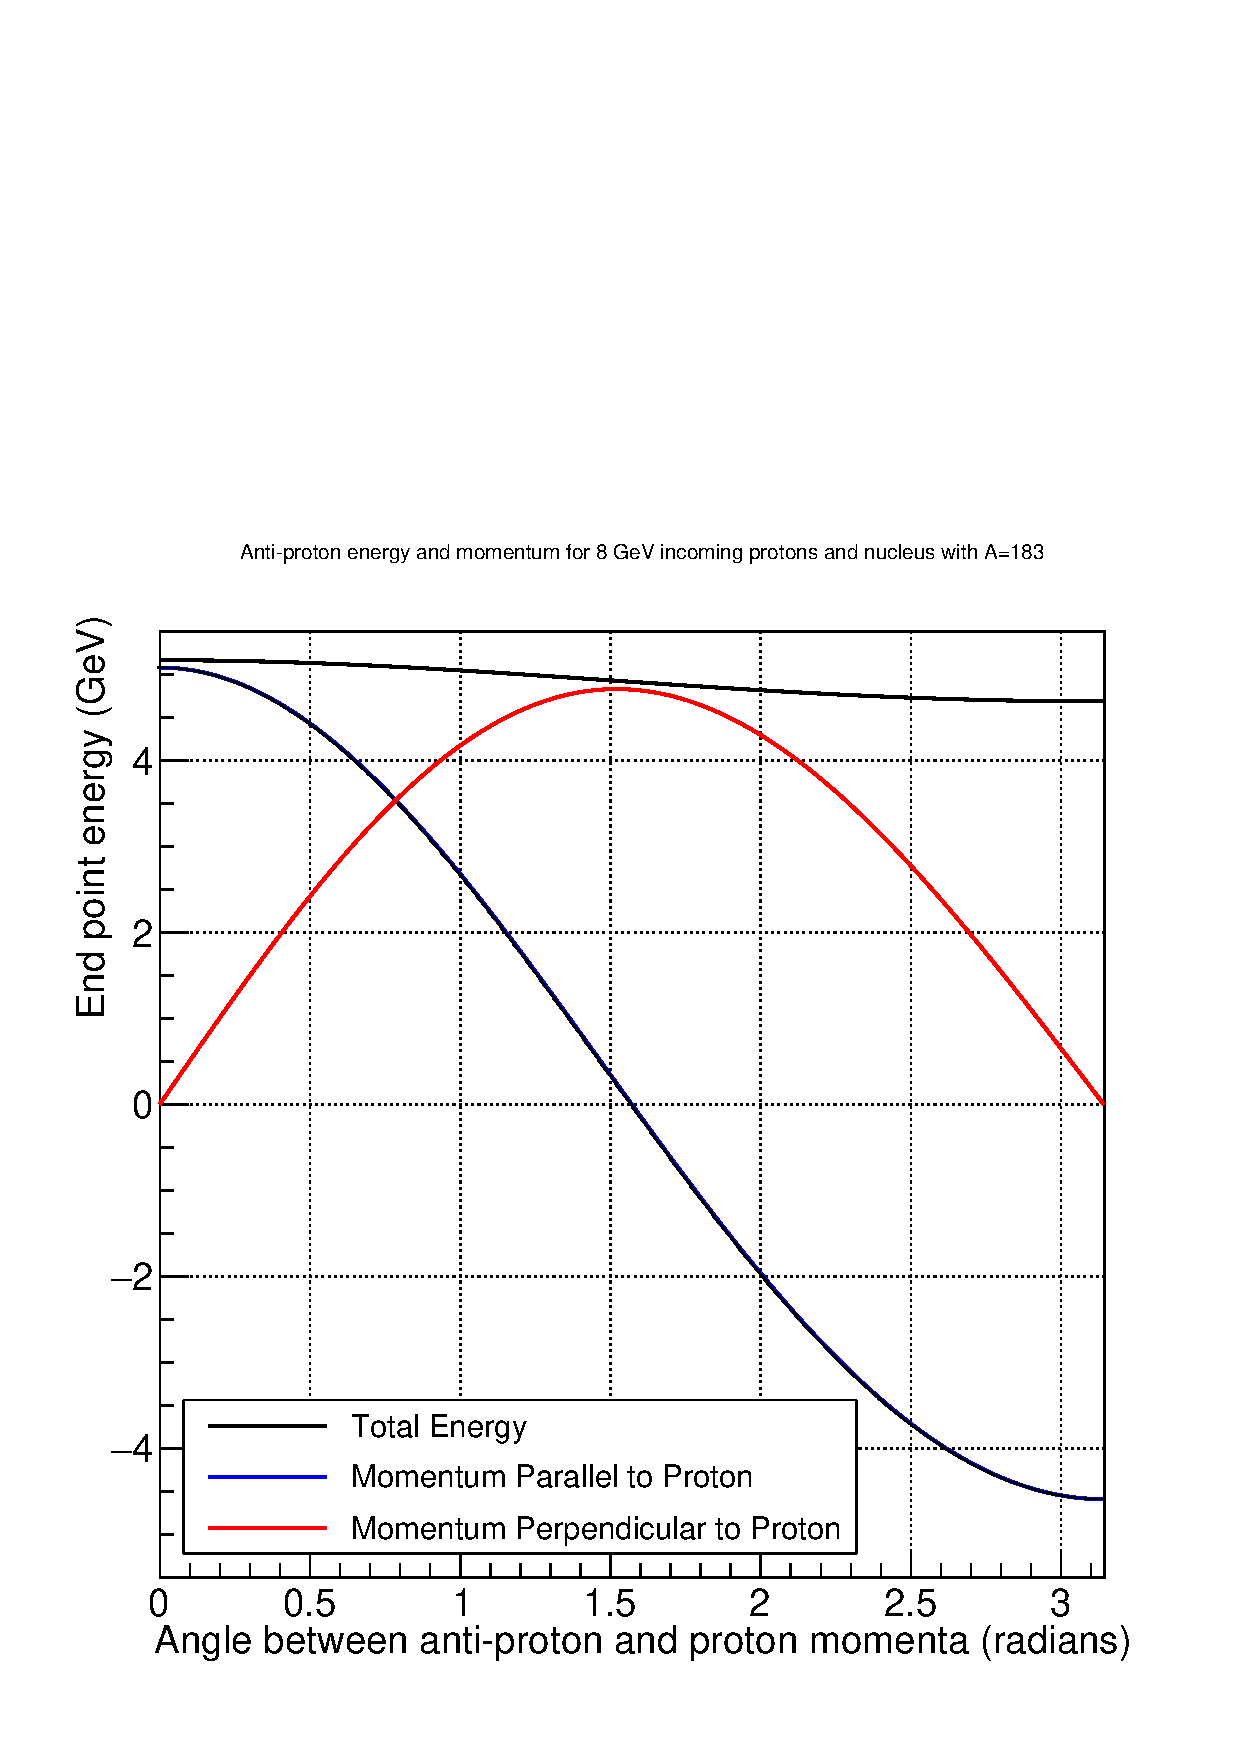
\includegraphics[width=0.49\textwidth,clip=true,trim=0 0 1cm 1.8cm]{figs/backgrounds/Antiproton_Tungsten_theta_lab.pdf}}%\hspace{0.5cm}%
\subfloat[][\figlabel{bg:antiprotons:end-point:carbon}Carbon    ]{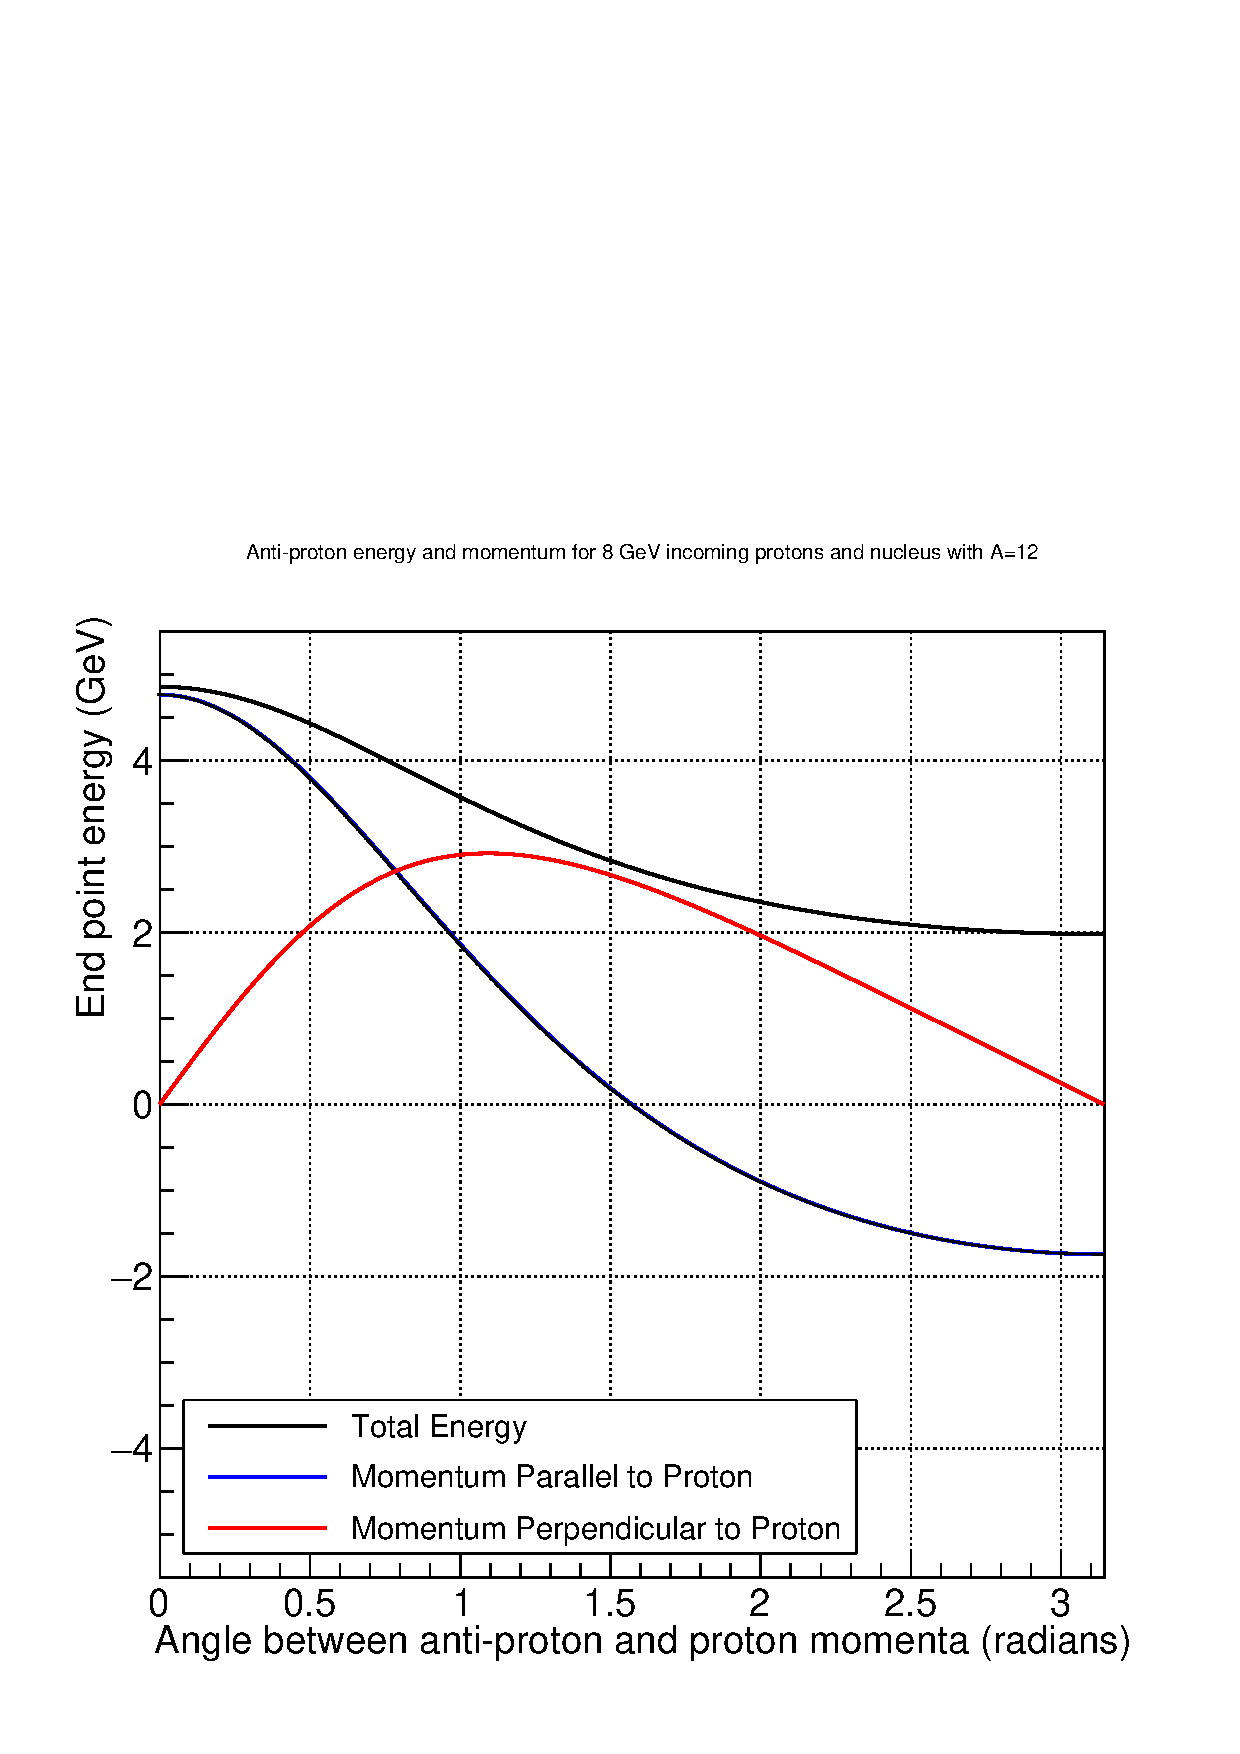
\includegraphics[width=0.49\textwidth,clip=true,trim=0 0 1cm 1.8cm]{figs/backgrounds/Antiproton_Carbon_theta_lab}}
\caption{\figlabel{bg:antiprotons:end-point}
The kinematic end-point for antiproton production as a function of the out-going antiproton direction with respect to the incoming proton in the frame of the target nucleus (the lab frame).
The absolute end-point is only achieved when the nucleus and out-going protons recoils coherently.
}
\end{figure}
}

\newcommand{\FigAntiprotonFits}{
\begin{figure}[tbp]
\centering
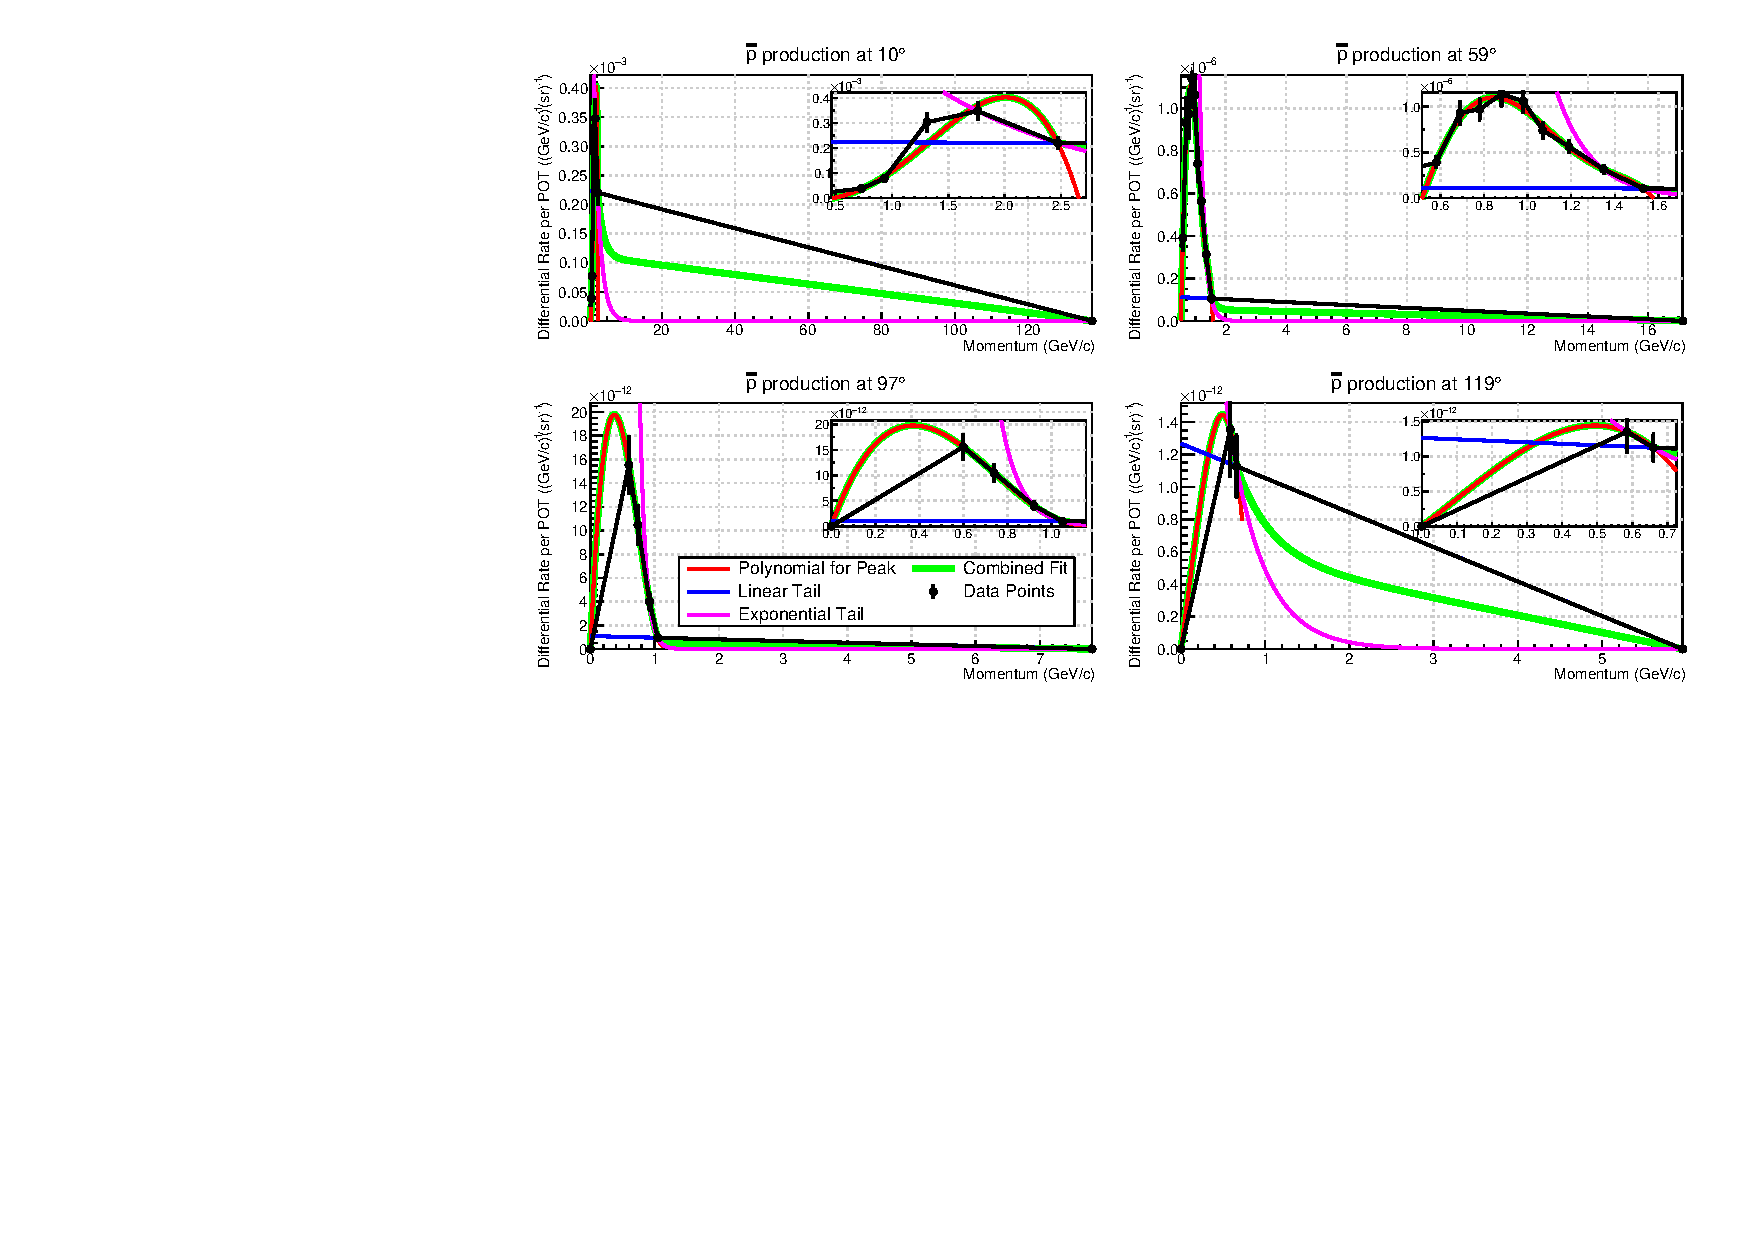
\includegraphics[width=1.0\textwidth,trim=0 0 0.45cm 0,clip]{figs/backgrounds/AntiprotonFits.pdf}
\caption{\figlabel{bg:antiprotons:fits}
Piecewise fitting to experimental data and kinematic end-points.
Inlays show a zoom around the experimental data points.
}
\end{figure}
}

\newcommand{\FigAntiprotonAngularDependence}{
\begin{figure}[tbp]
\centering
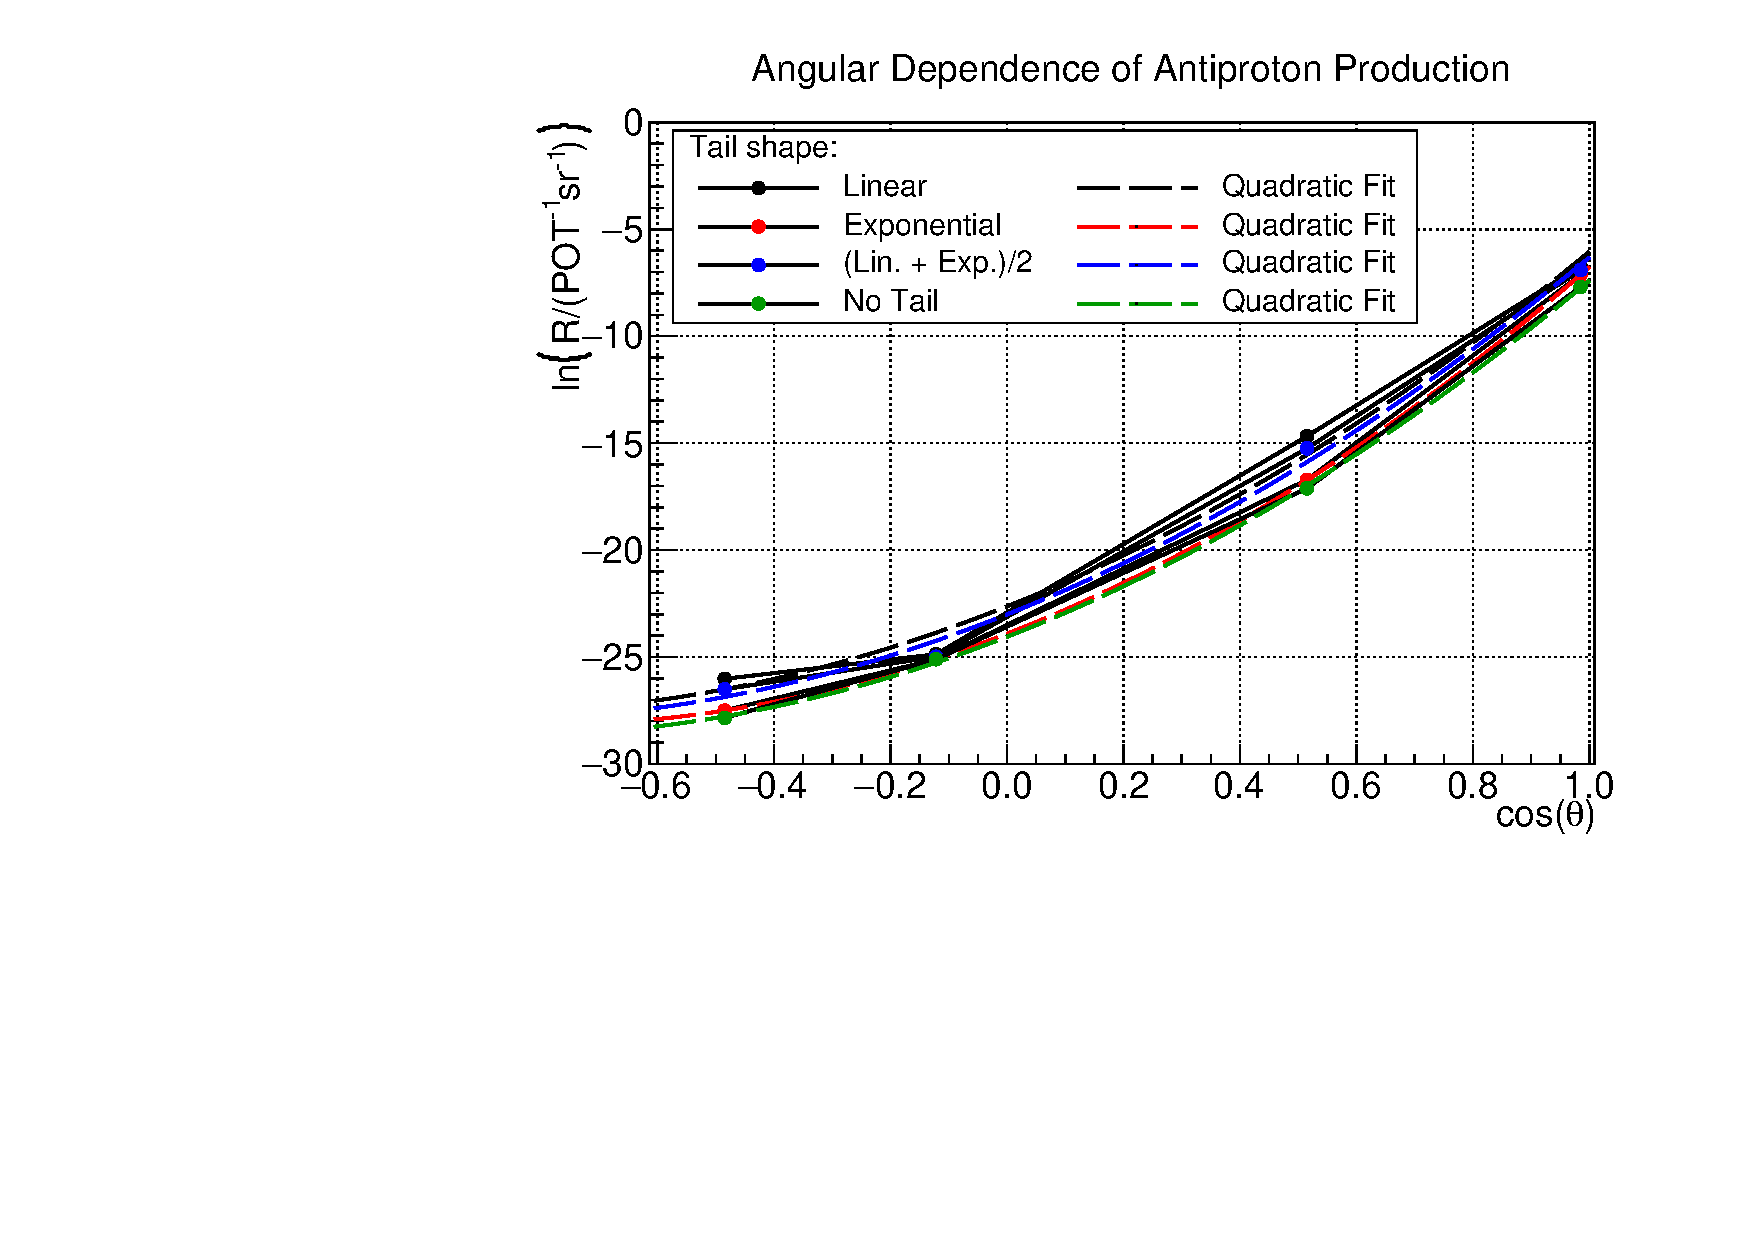
\includegraphics[width=0.8\textwidth,trim=0 0 1.4cm 1cm,clip]{figs/backgrounds/AntiprotonAngularDependence.pdf}
\caption{\figlabel{bg:antiprotons:angular}
The angular dependence of the rate of antiproton emission, integrated over all momenta.
The different lines represent the different fits to the high momentum part of the spectrum.
The relationship given in~\cite{Boyarinov:1994tp} would suggest the data here should fit a straight line.
The dashed lines represent instead a quadratic fit to these points, which looks like a better fit.
For reweighting events the interpolated (straight solid) lines were used to be conservative.
}
\end{figure}
}

\newcommand{\TabAntiprotonRegions}{
\begin{table}[bp]
\centering
	\begin{tabular}{rclrS}
		\multicolumn{3}{c}{Region} & Data source & \multicolumn{1}{r}{Total $\bar{p}$ per POT} \\
\hline
                  $0 \le$&$\theta<$&$59\degree$ & 10\degree \cite{Kiselev:2012sj}          & 5.26e-05\\
                 $59 \le$&$\theta<$&$97\degree$ & 59\degree \cite{Kiselev:2012sj}         & 4.17e-09\\
                 $97 \le$&$\theta<$&$119\degree$ & 97\degree \cite{Boyarinov:1994tp}      & 1.74e-12\\
                $119 \le$&$\theta<$&$180\degree$ & 119\degree \cite{Boyarinov:1994tp}   & 5.71e-13\\
\hline
\end{tabular}
\caption{\tablabel{bg:antiprotons:regions}
Regions and fits used to simulate antiproton production.  
The values in the final column are result of converting to rates per POT and integrating the differential cross-sections measured in \cite{Boyarinov:1994tp,Kiselev:2012sj}.
%integrated the fitted and extrapolated spectra and then integrates over the fitted angular dependence.
}
\end{table}
}

\newcommand{\FigAntiprotonSimHeightsTwoDPbar}{%
\begin{figure}[pH]%
\centering %
\subfloat[][\figlabel{bg:antiprotons:sim:2D-antip:10}Production between 0 and 59\degree]{%
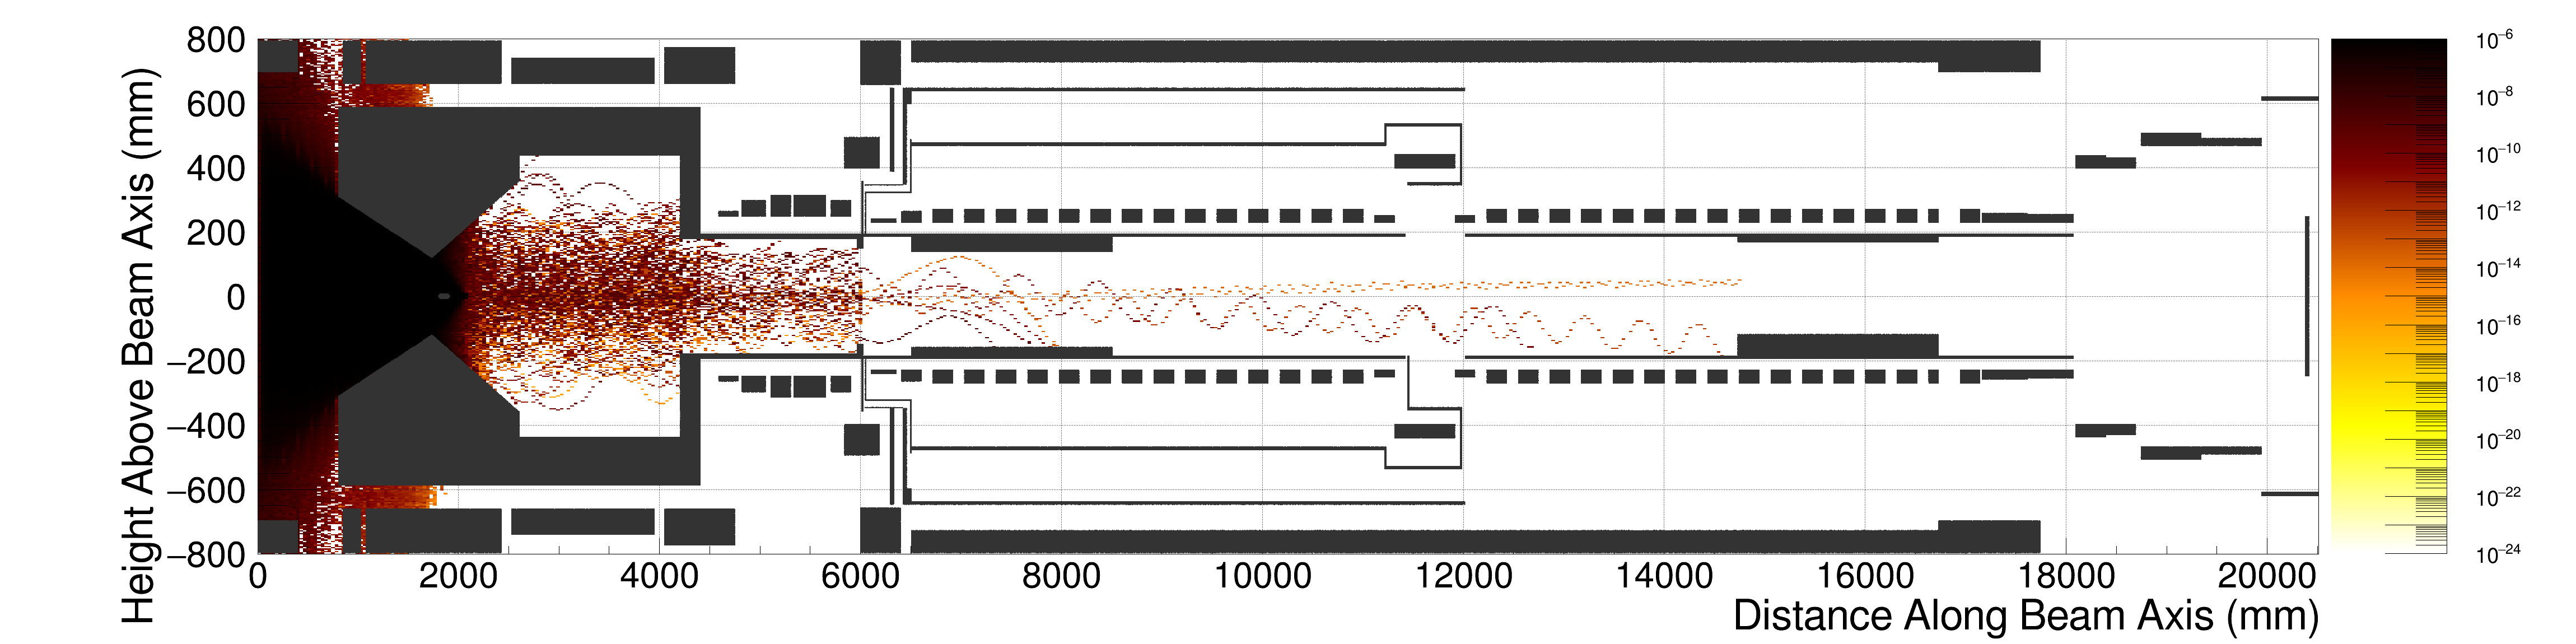
\includegraphics[width=1\textwidth,trim=3.7cm 0.3cm 1.8cm 0.8cm,clip]{figs/backgrounds/Antiproton_height2D_antiproton_10.png}}\\%
\subfloat[][\figlabel{bg:antiprotons:sim:2D-antip:59}Production between 59 and 97\degree]{%
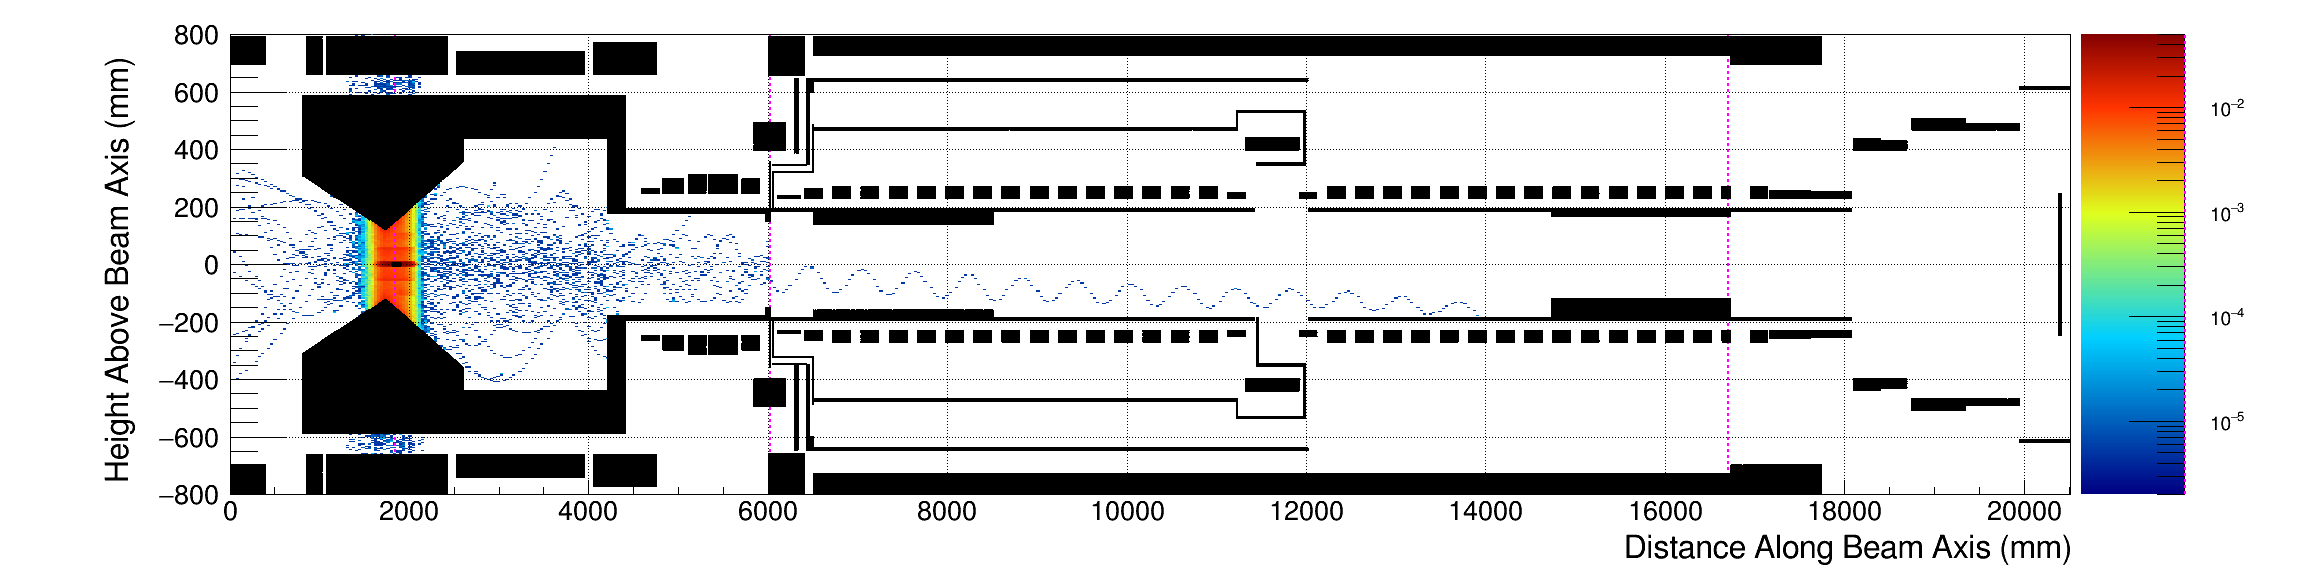
\includegraphics[width=1\textwidth,trim=3.7cm 0.3cm 1.8cm 0.8cm,clip]{figs/backgrounds/Antiproton_height2D_antiproton_59.png}}\\%
\subfloat[][\figlabel{bg:antiprotons:sim:2D-antip:97}Production between 97 and 119\degree]{%
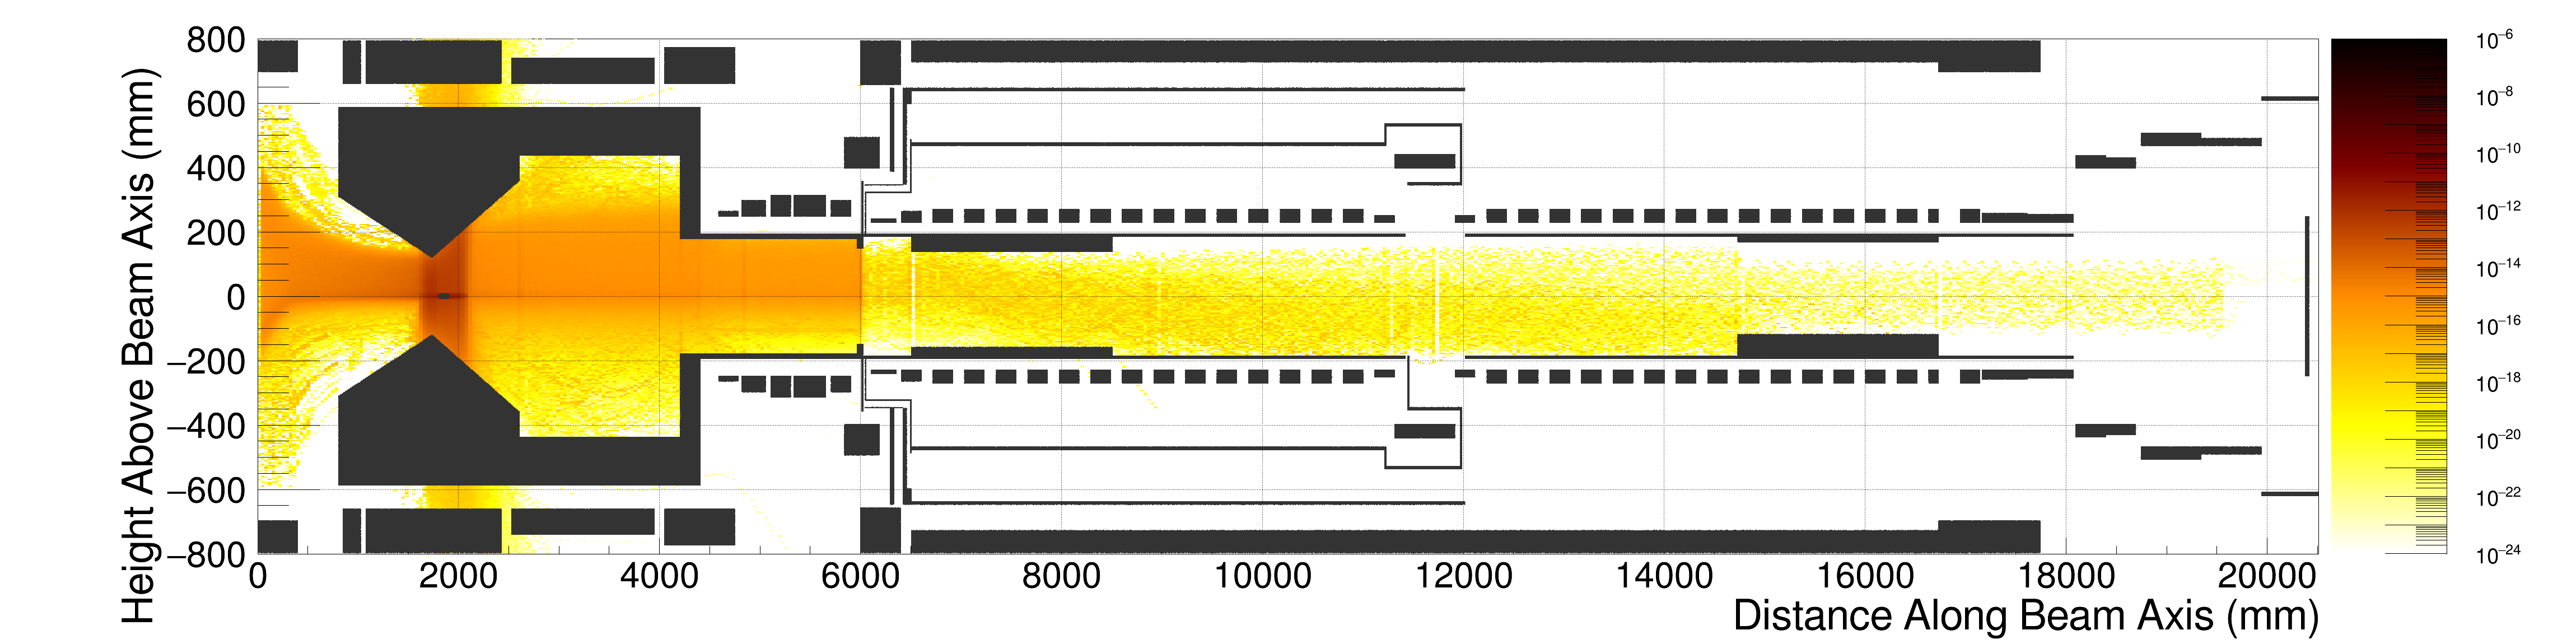
\includegraphics[width=1\textwidth,trim=3.7cm 0.3cm 1.8cm 0.8cm,clip]{figs/backgrounds/Antiproton_height2D_antiproton_97.png}}\\%
\subfloat[][\figlabel{bg:antiprotons:sim:2D-antip:119}Production between 119 and 180\degree]{%
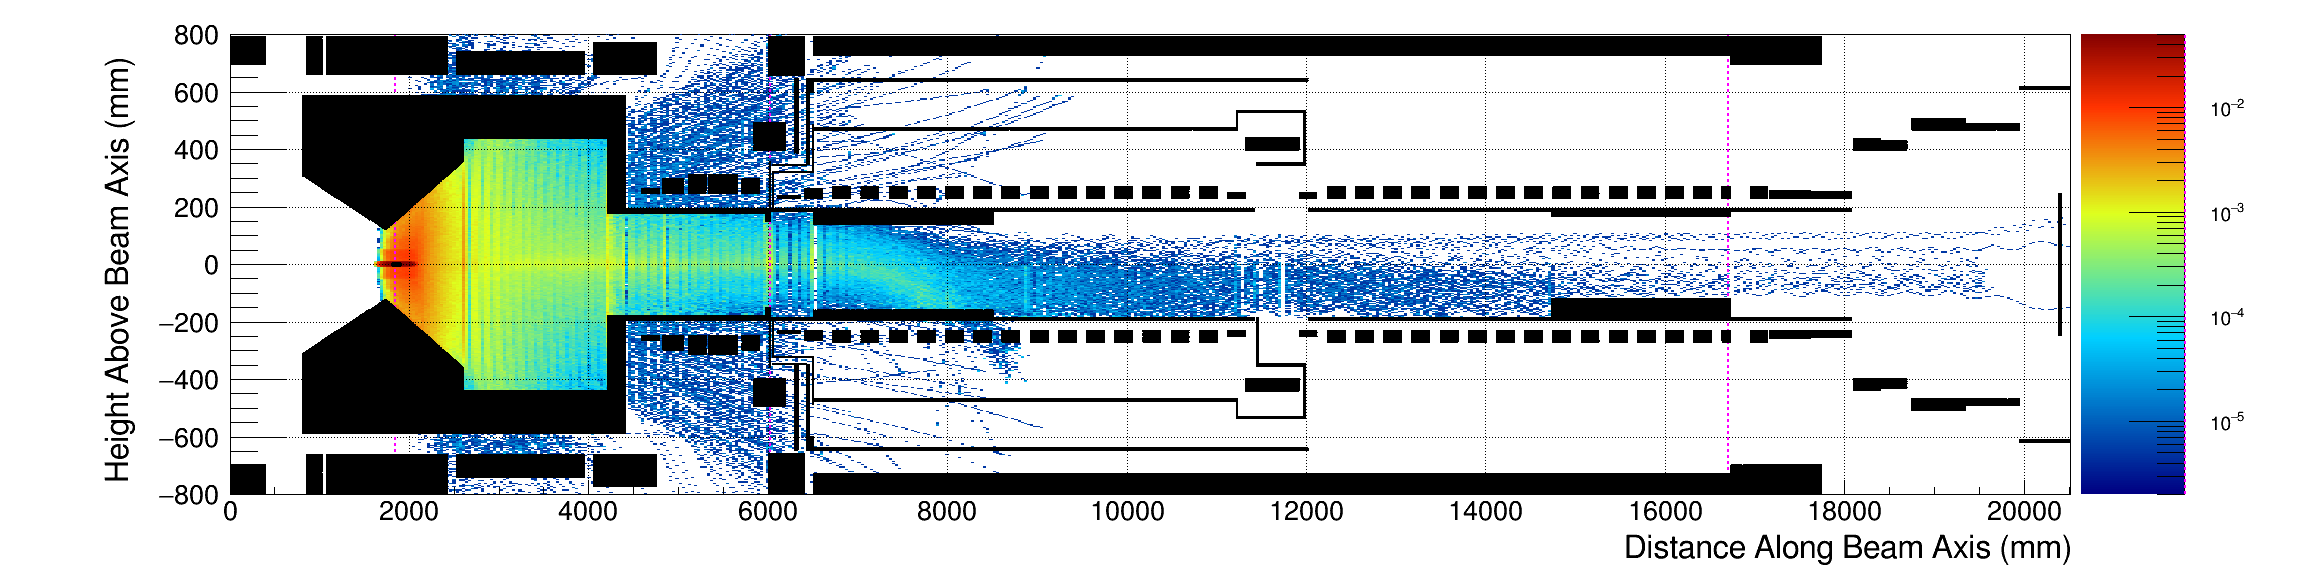
\includegraphics[width=1\textwidth,trim=3.7cm 0.3cm 1.8cm 0.8cm,clip]{figs/backgrounds/Antiproton_height2D_antiproton_119.png}}%
\caption{\figlabel{bg:antiprotons:sim:2D-antip}%
The heights of antiprotons passing along the beamline for the four different angular regions of productions.%
Each antiproton trajectory is weighted by the probability of producing an antiproton at this angle.%
The colour scale on all these plots is the same.%
}%
\end{figure}%
\xspace}

\newcommand{\FigAntiprotonSimHeightsTwoDPiMin}{%
\begin{figure}[pH]%
\centering %
\subfloat[][\figlabel{bg:antiprotons:sim:2D-pi:10}Production between 0 and 59\degree]{%
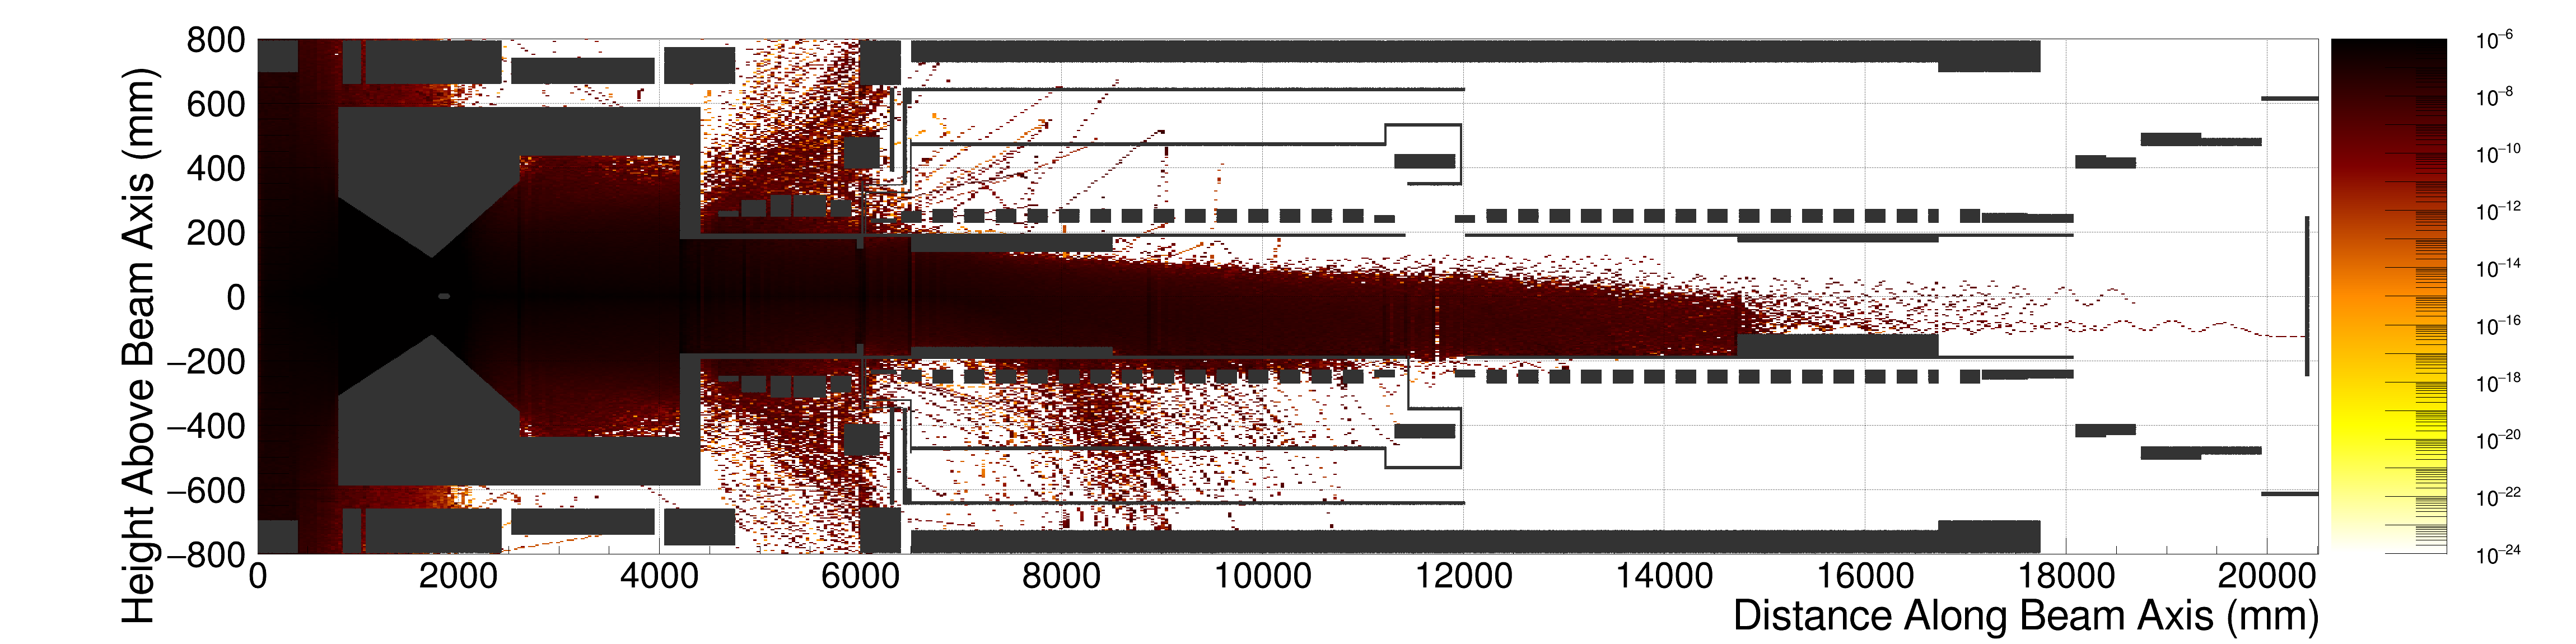
\includegraphics[width=1\textwidth,trim=3.7cm 0.3cm 1.8cm 0.8cm,clip]{figs/backgrounds/Antiproton_height2D_pi-_10.png}}\\%
\subfloat[][\figlabel{bg:antiprotons:sim:2D-pi:59}Production between 59 and 97\degree]{%
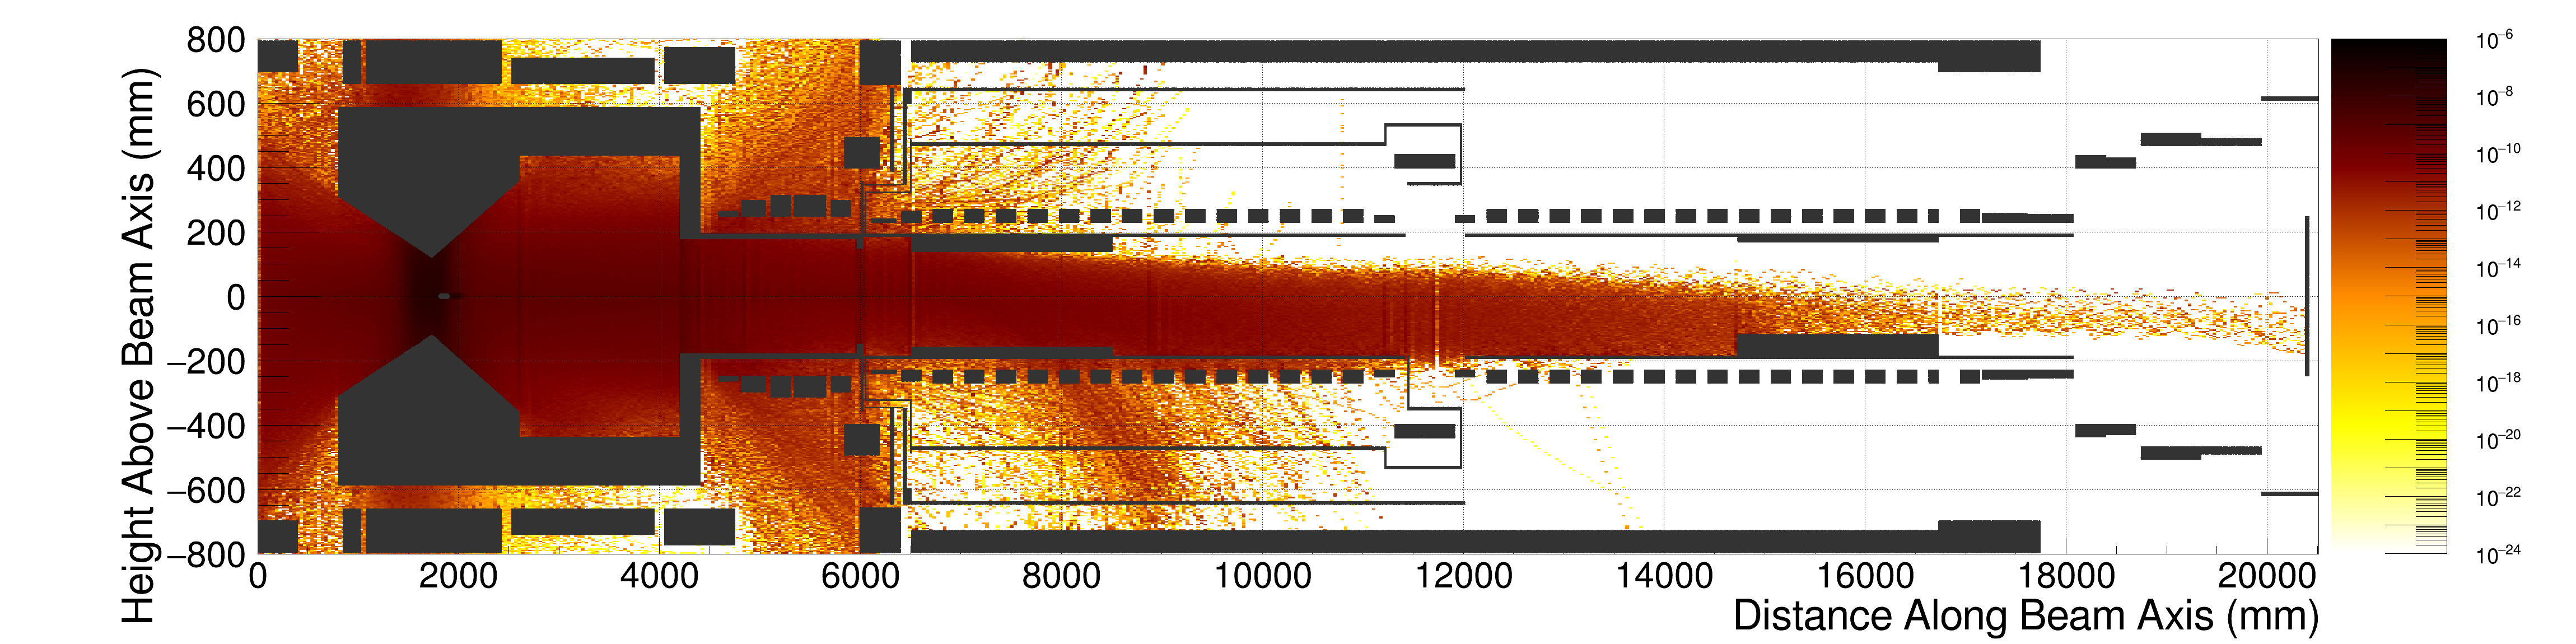
\includegraphics[width=1\textwidth,trim=3.7cm 0.3cm 1.8cm 0.8cm,clip]{figs/backgrounds/Antiproton_height2D_pi-_59.png}}\\%
\subfloat[][\figlabel{bg:antiprotons:sim:2D-pi:97}Production between 97 and 119\degree]{%
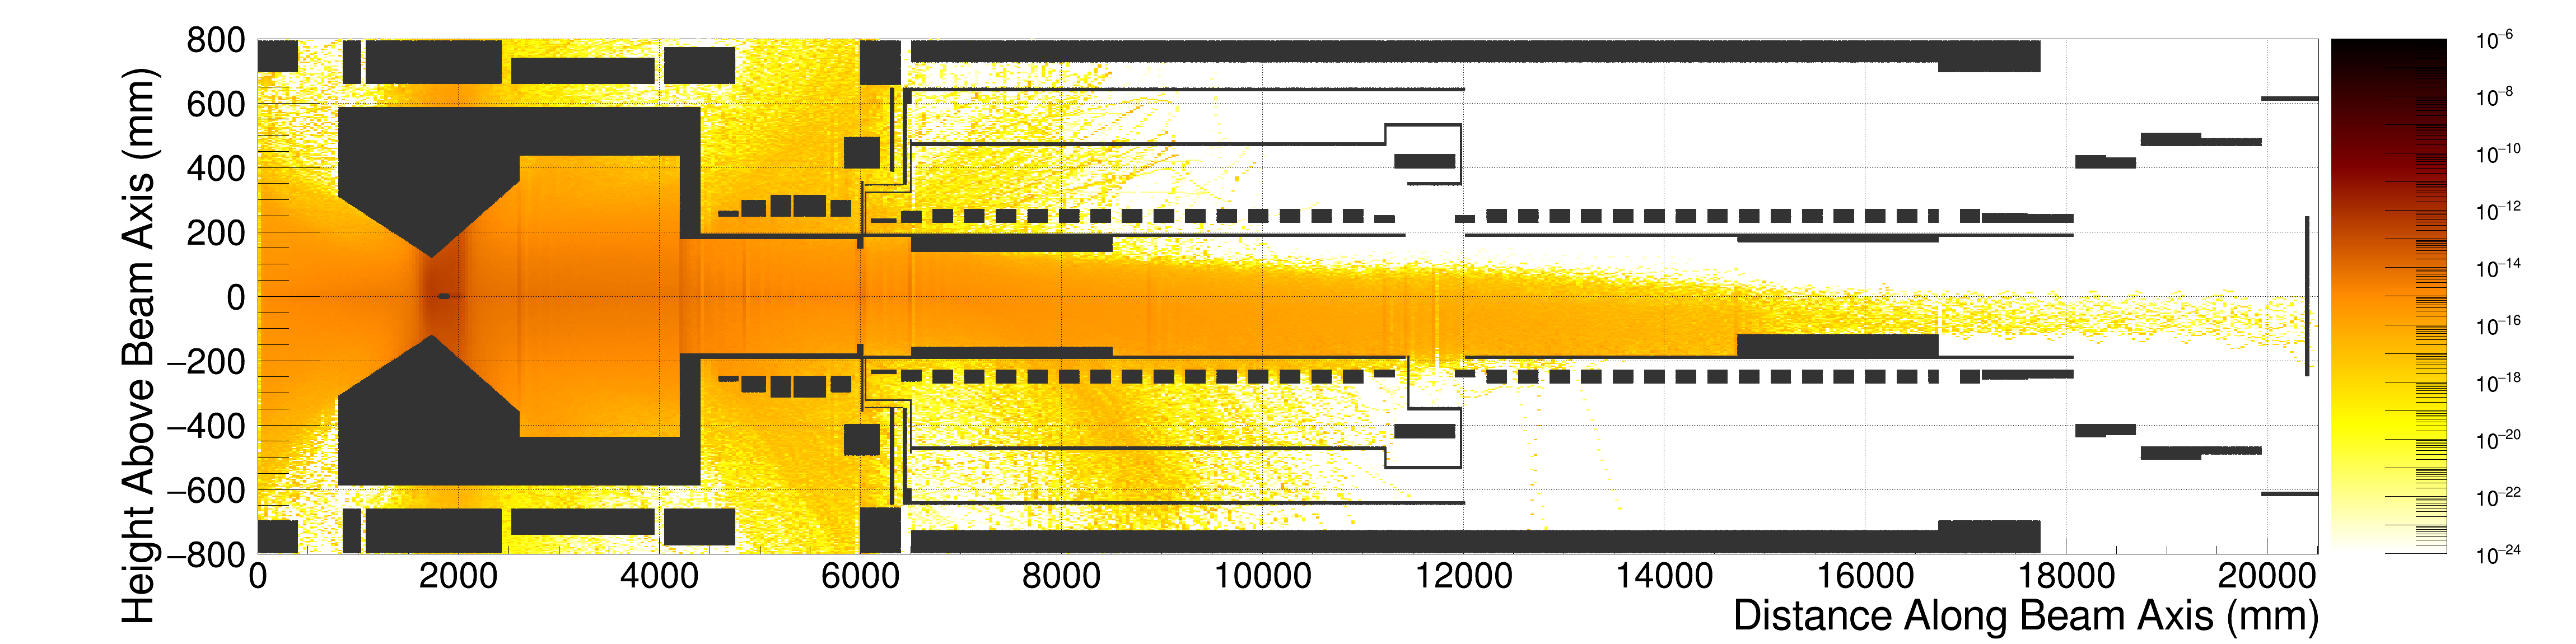
\includegraphics[width=1\textwidth,trim=3.7cm 0.3cm 1.8cm 0.8cm,clip]{figs/backgrounds/Antiproton_height2D_pi-_97.png}}\\%
\subfloat[][\figlabel{bg:antiprotons:sim:2D-pi:119}Production between 119 and 180\degree]{%
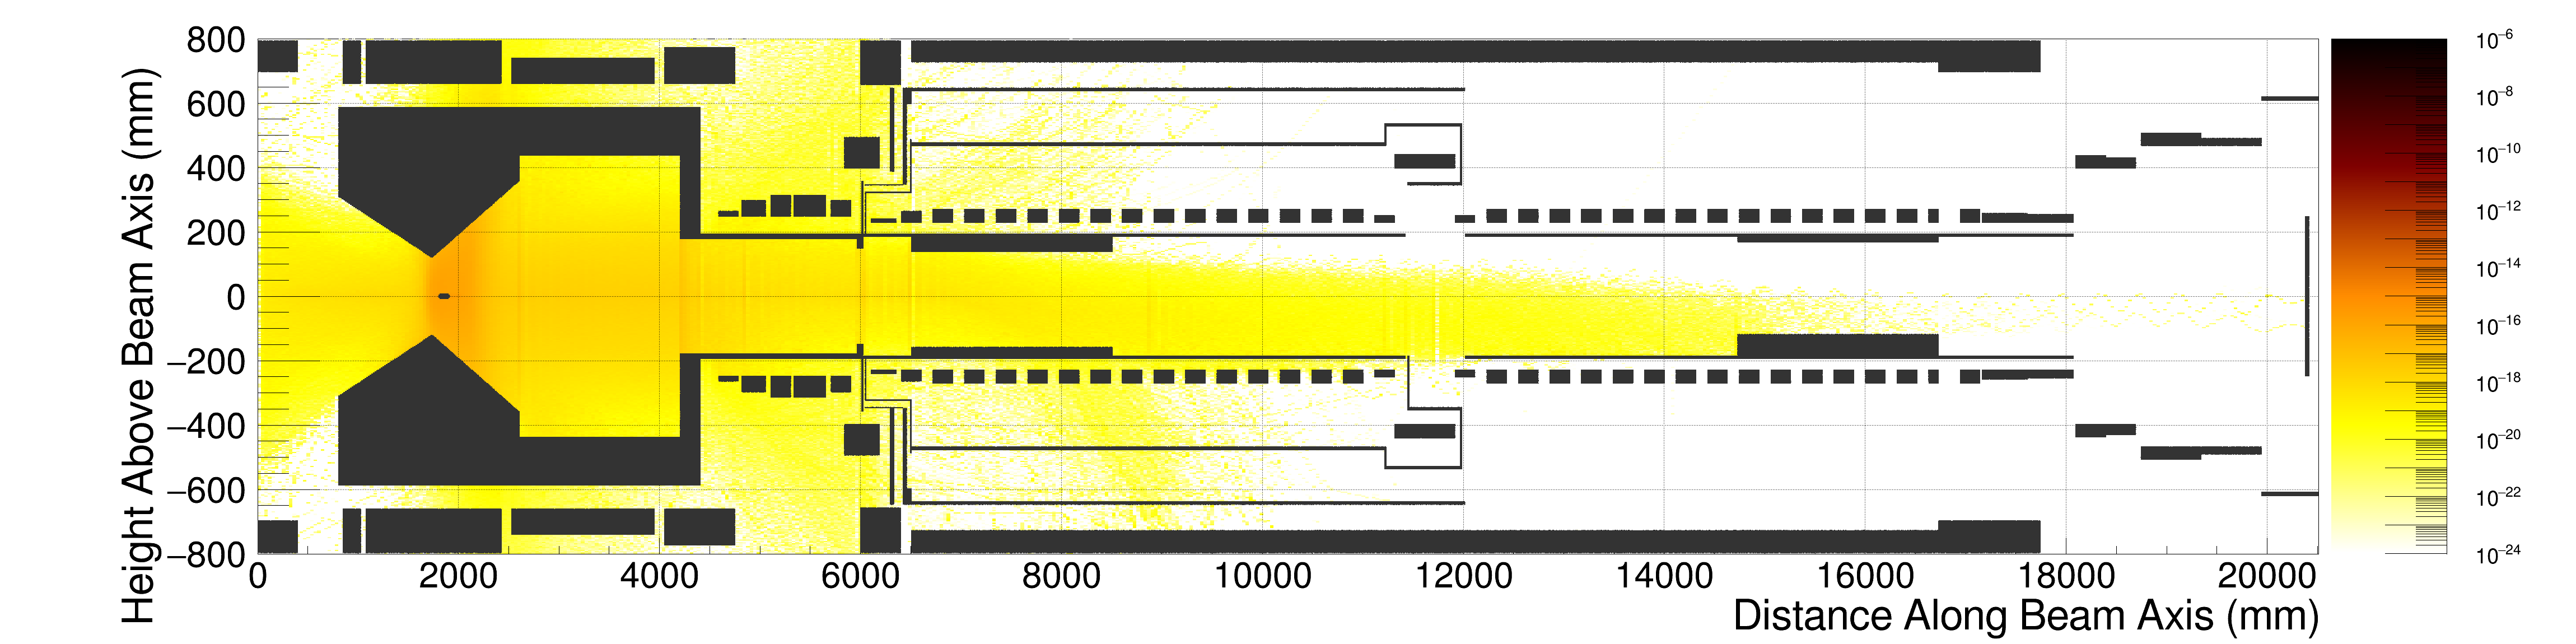
\includegraphics[width=1\textwidth,trim=3.7cm 0.3cm 1.8cm 0.8cm,clip]{figs/backgrounds/Antiproton_height2D_pi-_119.png}}%
\caption{\figlabel{bg:antiprotons:sim:2D-pi}%
The heights of secondary pions passing along the beamline produced from antiprotons in each of the four different angular regions of productions.%
Each antiproton trajectory is weighted by the probability of producing the parent antiproton in its initial direction at the target.%
}%
\end{figure}%
\xspace}%

\newcommand{\FigAntiprotonSimFluxes}{
\begin{figure}[b]
\centering 
\subfloat[][\figlabel{bg:antiprotons:sim:fluxes:antip}Unweighted Antiproton Survival Probability]{
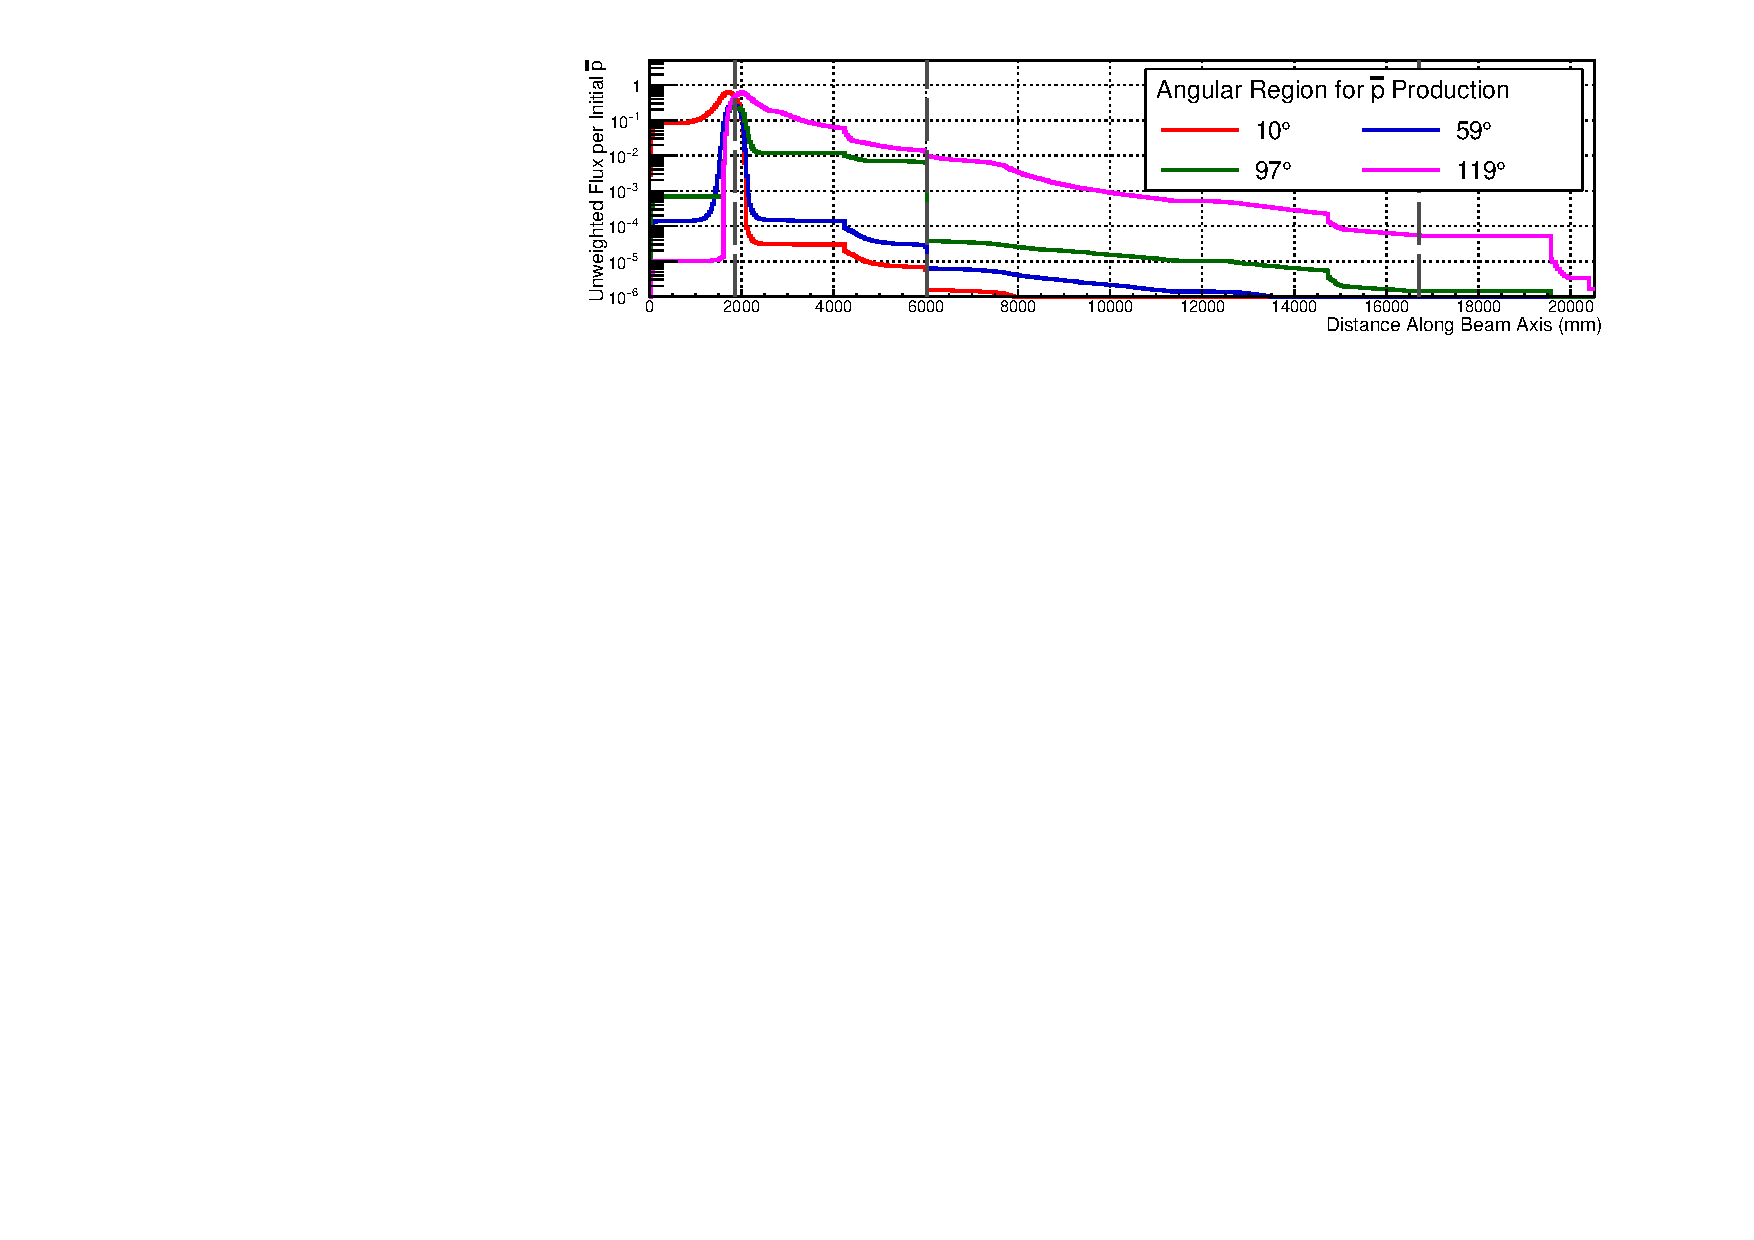
\includegraphics[width=1\textwidth,trim=0.7cm 0 1.9cm 0.2cm,clip]{figs/backgrounds/Antiproton_fluxes.pdf}}\\
\subfloat[][\figlabel{bg:antiprotons:sim:fluxes:pion}Unweighted Secondary Pion Transport Probability]{
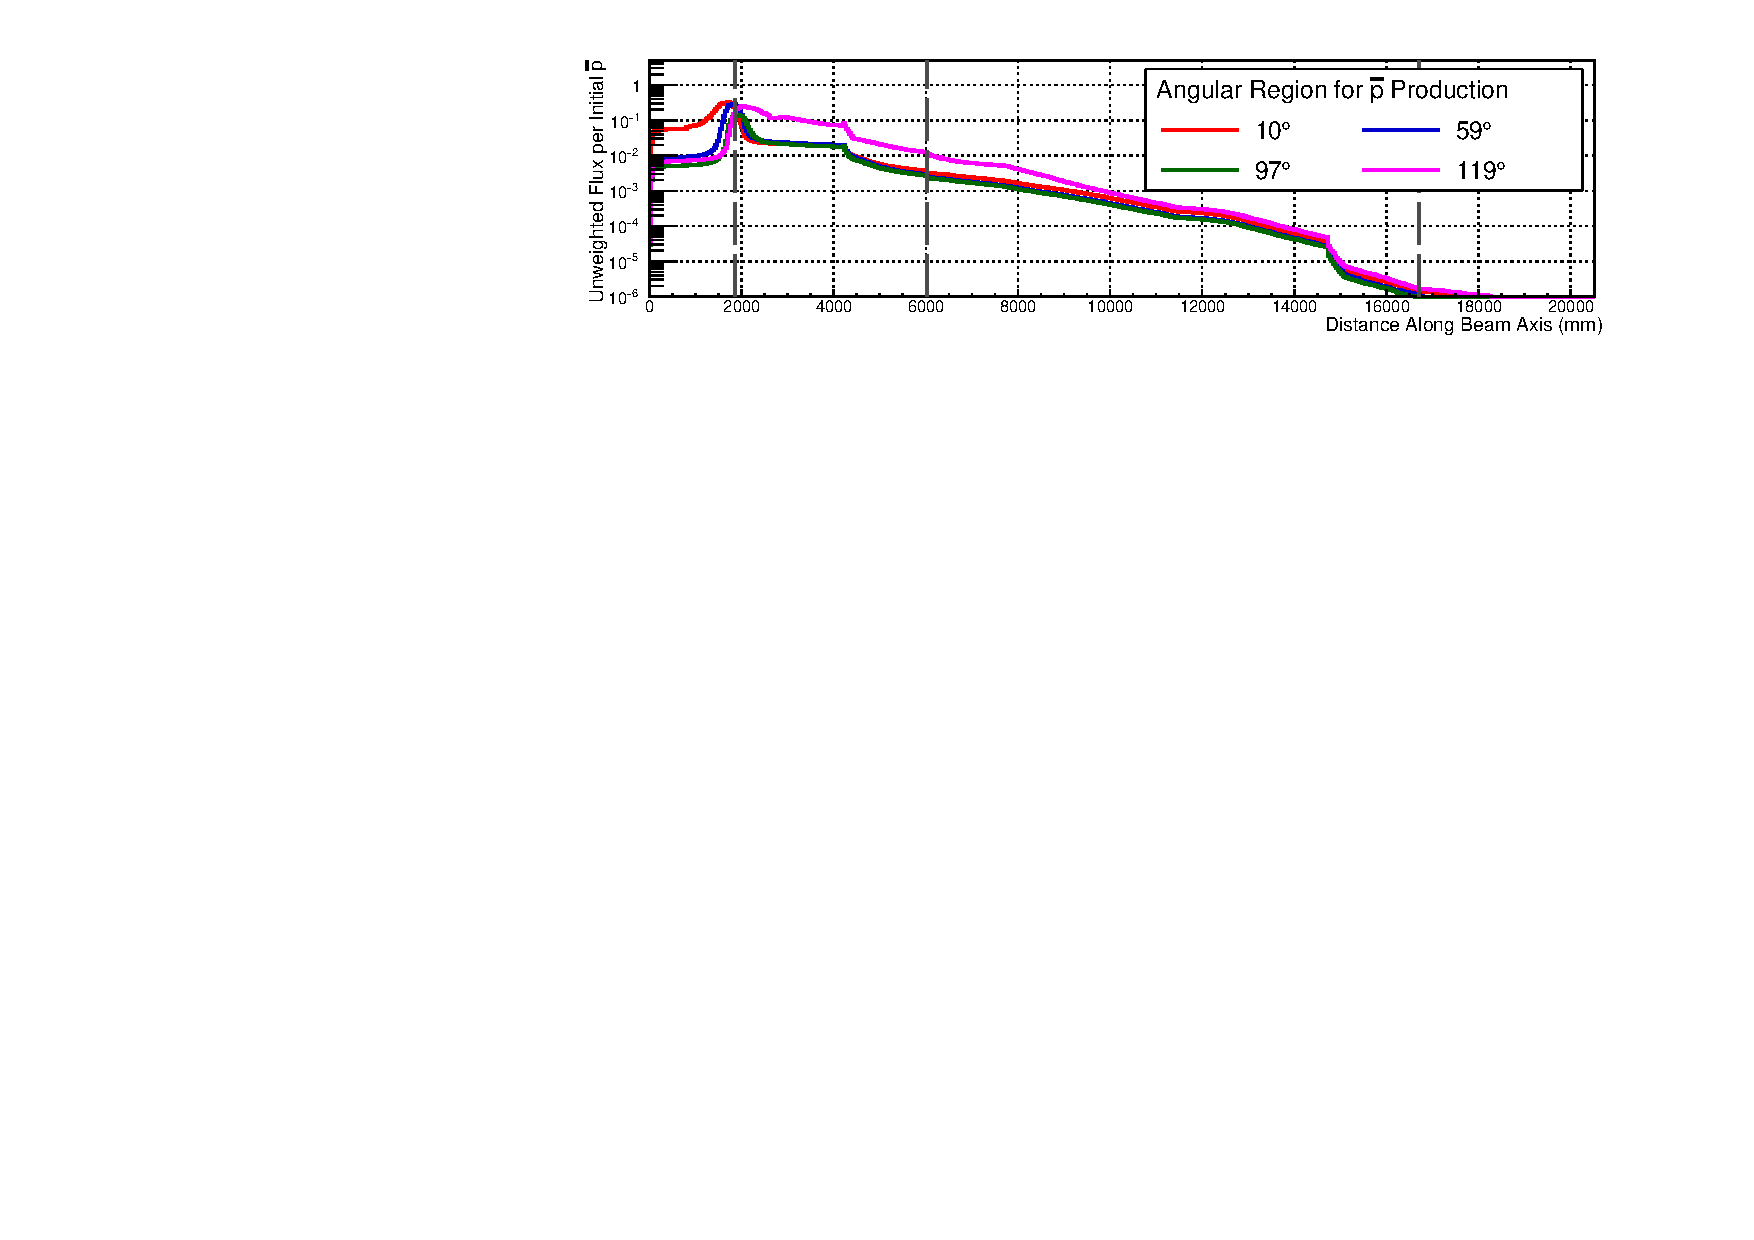
\includegraphics[width=1\textwidth,trim=0.7cm 0 1.9cm 0.2cm,clip]{figs/backgrounds/Antiproton_fluxes-pions.pdf}}
\caption{\figlabel{bg:antiprotons:sim:fluxes}
The surivival probability of antiprotons and secondaries pions per antiproton produced in the target as a function of distance along the beamline.
These plots are not weighted by the probability that an antiproton is produced at a particular angle.
From left to right the vertical gray lines indicate the production target, Torus1 entrance, and the Torus2 exit.
}
\end{figure}
}

\newcommand{\FigAntiprotonSimTime}{
\begin{figure}[t]
\centering 
\subfloat[][\figlabel{bg:antiprotons:sim:time:antip}Timing of Antiprotons]{
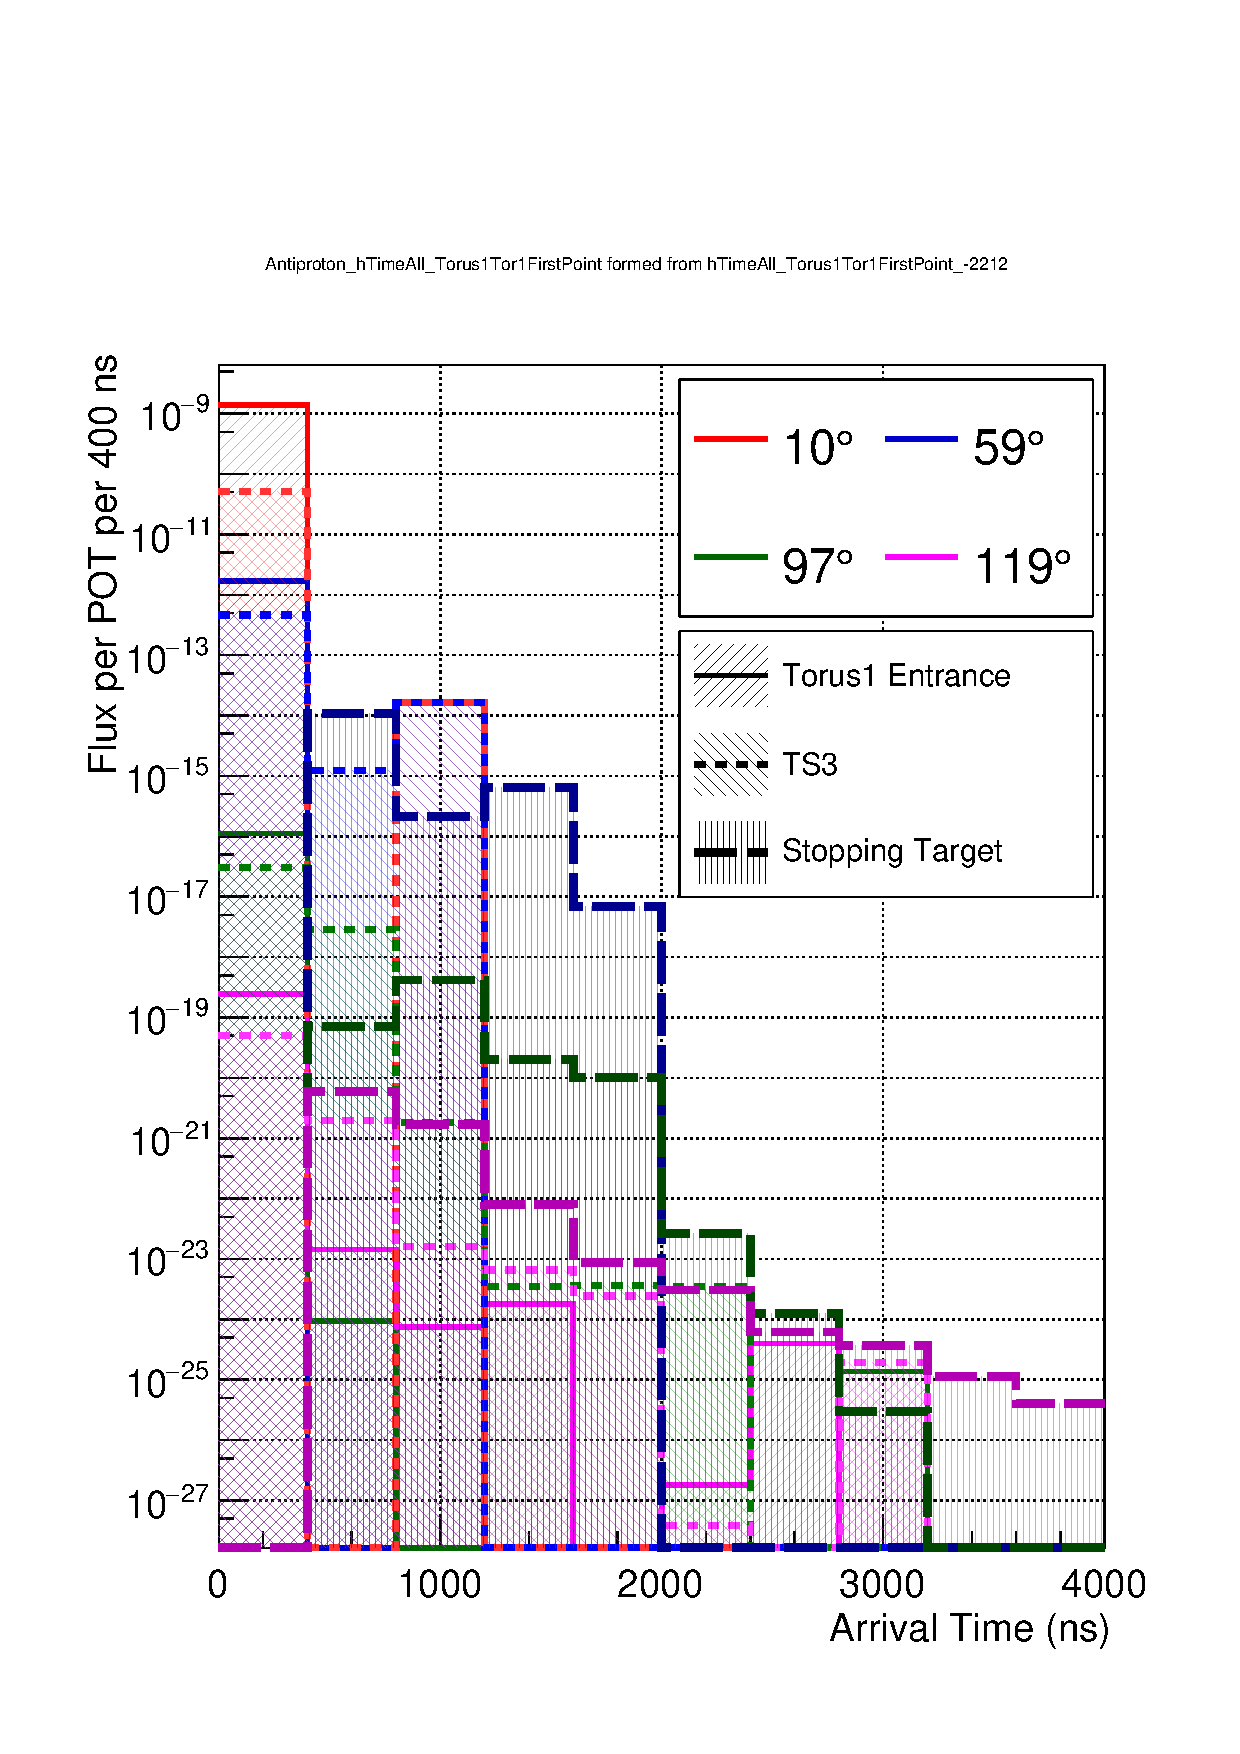
\includegraphics[width=0.45\textwidth,trim=0.7cm 0.5cm 1.3cm 1.7cm,clip]{figs/backgrounds/Antiproton_timing_antiprotons.pdf}}
\subfloat[][\figlabel{bg:antiprotons:sim:time:pion}Timing of Secondary Pions]{
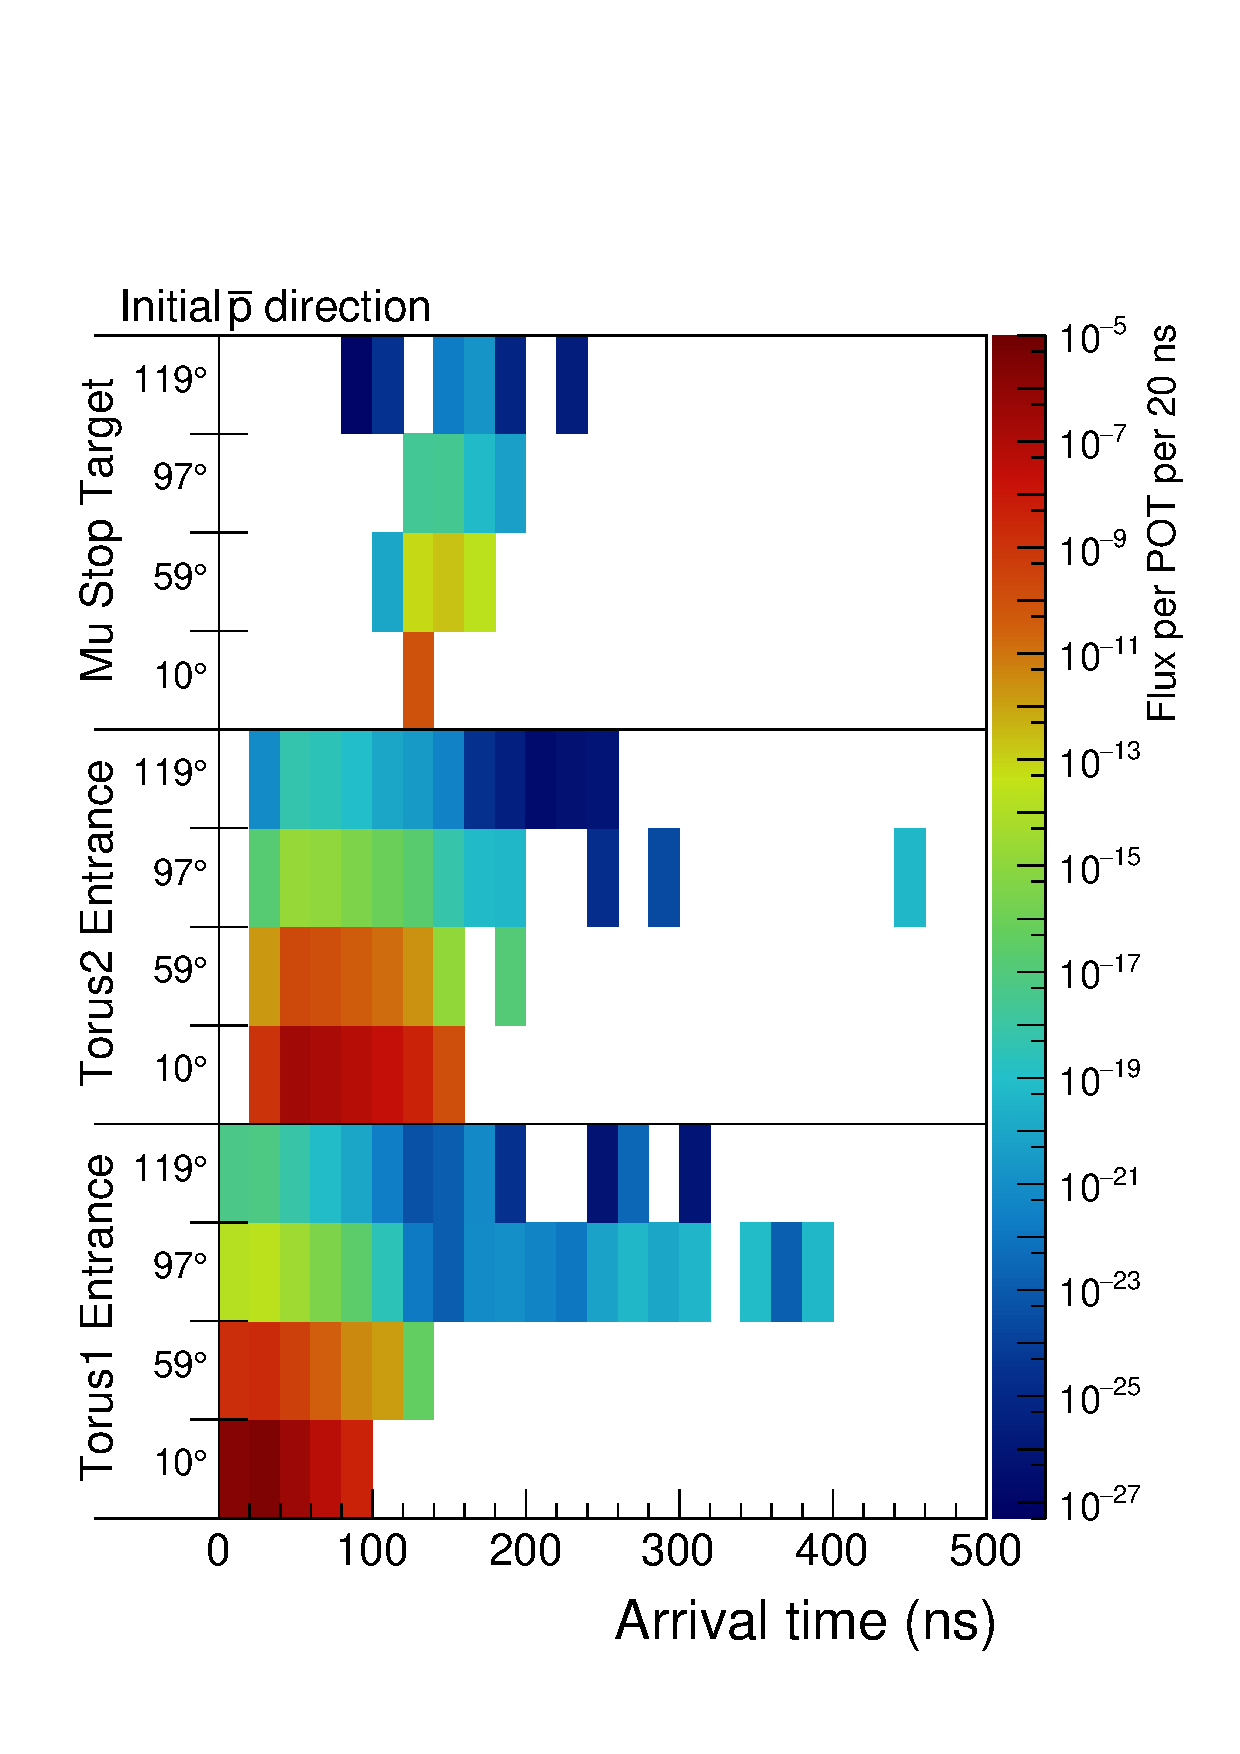
\includegraphics[width=0.45\textwidth,trim=0.7cm 0.5cm 1.3cm 1.7cm,clip]{figs/backgrounds/Antiproton_timing_pions.pdf}}
\caption{\figlabel{bg:antiprotons:sim:time}
\CHECK{Add pion stopping timing to RPC section to be able to compare to it here}
The arrival time of antiprotons and pions at the entrance to the bent solenoids (Torus1 Entrance), at the midpoint (TS3), and at the stopping target.
Note that the x-axis scales are different.
Whilst the timing of antiprotons themselves is very delayed, the timing of pions, which are produced predominantly at the production target, is relatively prompt and will be effective at suppressing the induced backgrounds.
}
\end{figure}
}

%\newcommand{\FigAntiprotonSimFluxes}{
%\begin{figure}[pH]
%\centering 
%\subfloat[][\figlabel{bg:antiprotons:sim:fluxes:10}Production between 0 and 59\degree]{
%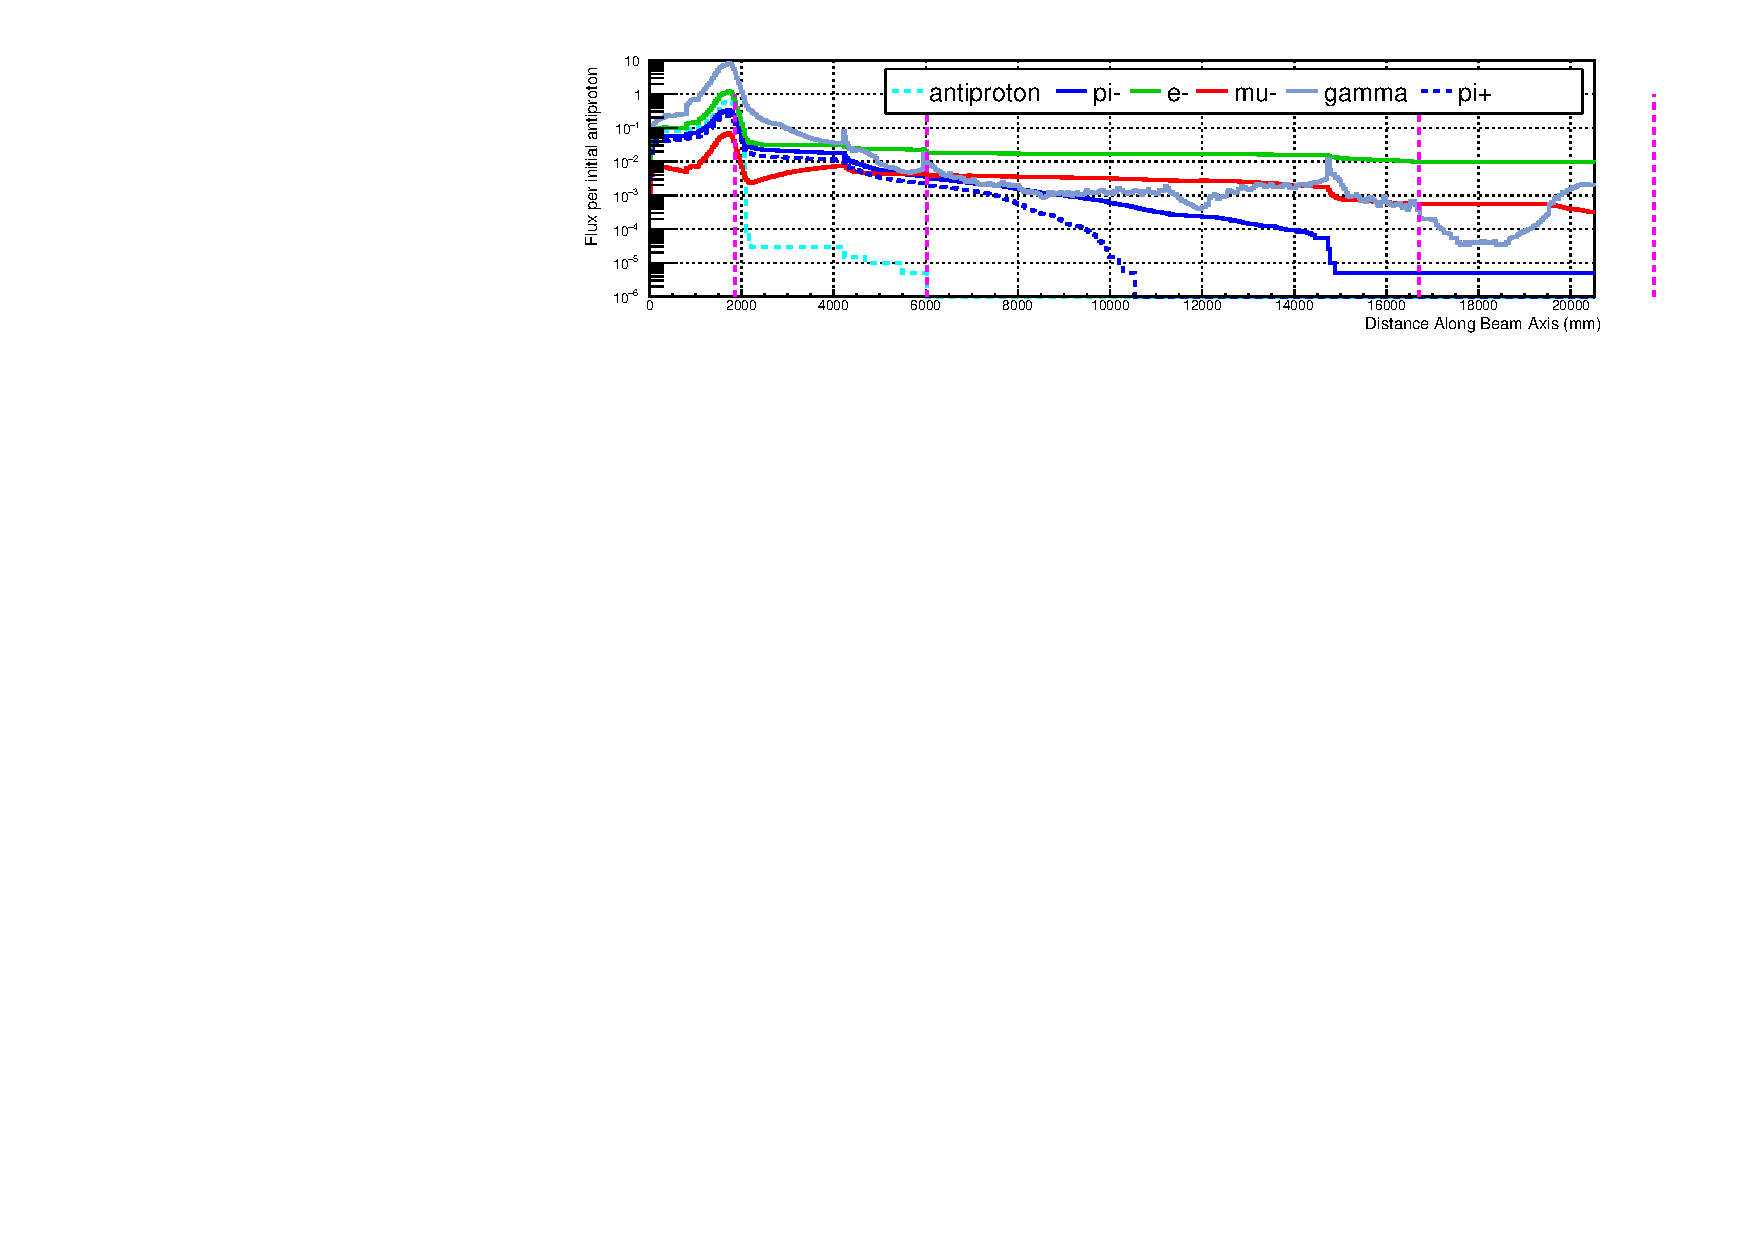
\includegraphics[width=1\textwidth,trim=0.7cm 0 1.9cm 0.2cm,clip]{figs/backgrounds/Antiproton_flux_10.pdf}}\\
%\subfloat[][\figlabel{bg:antiprotons:sim:fluxes:59}Production between 59 and 97\degree]{
%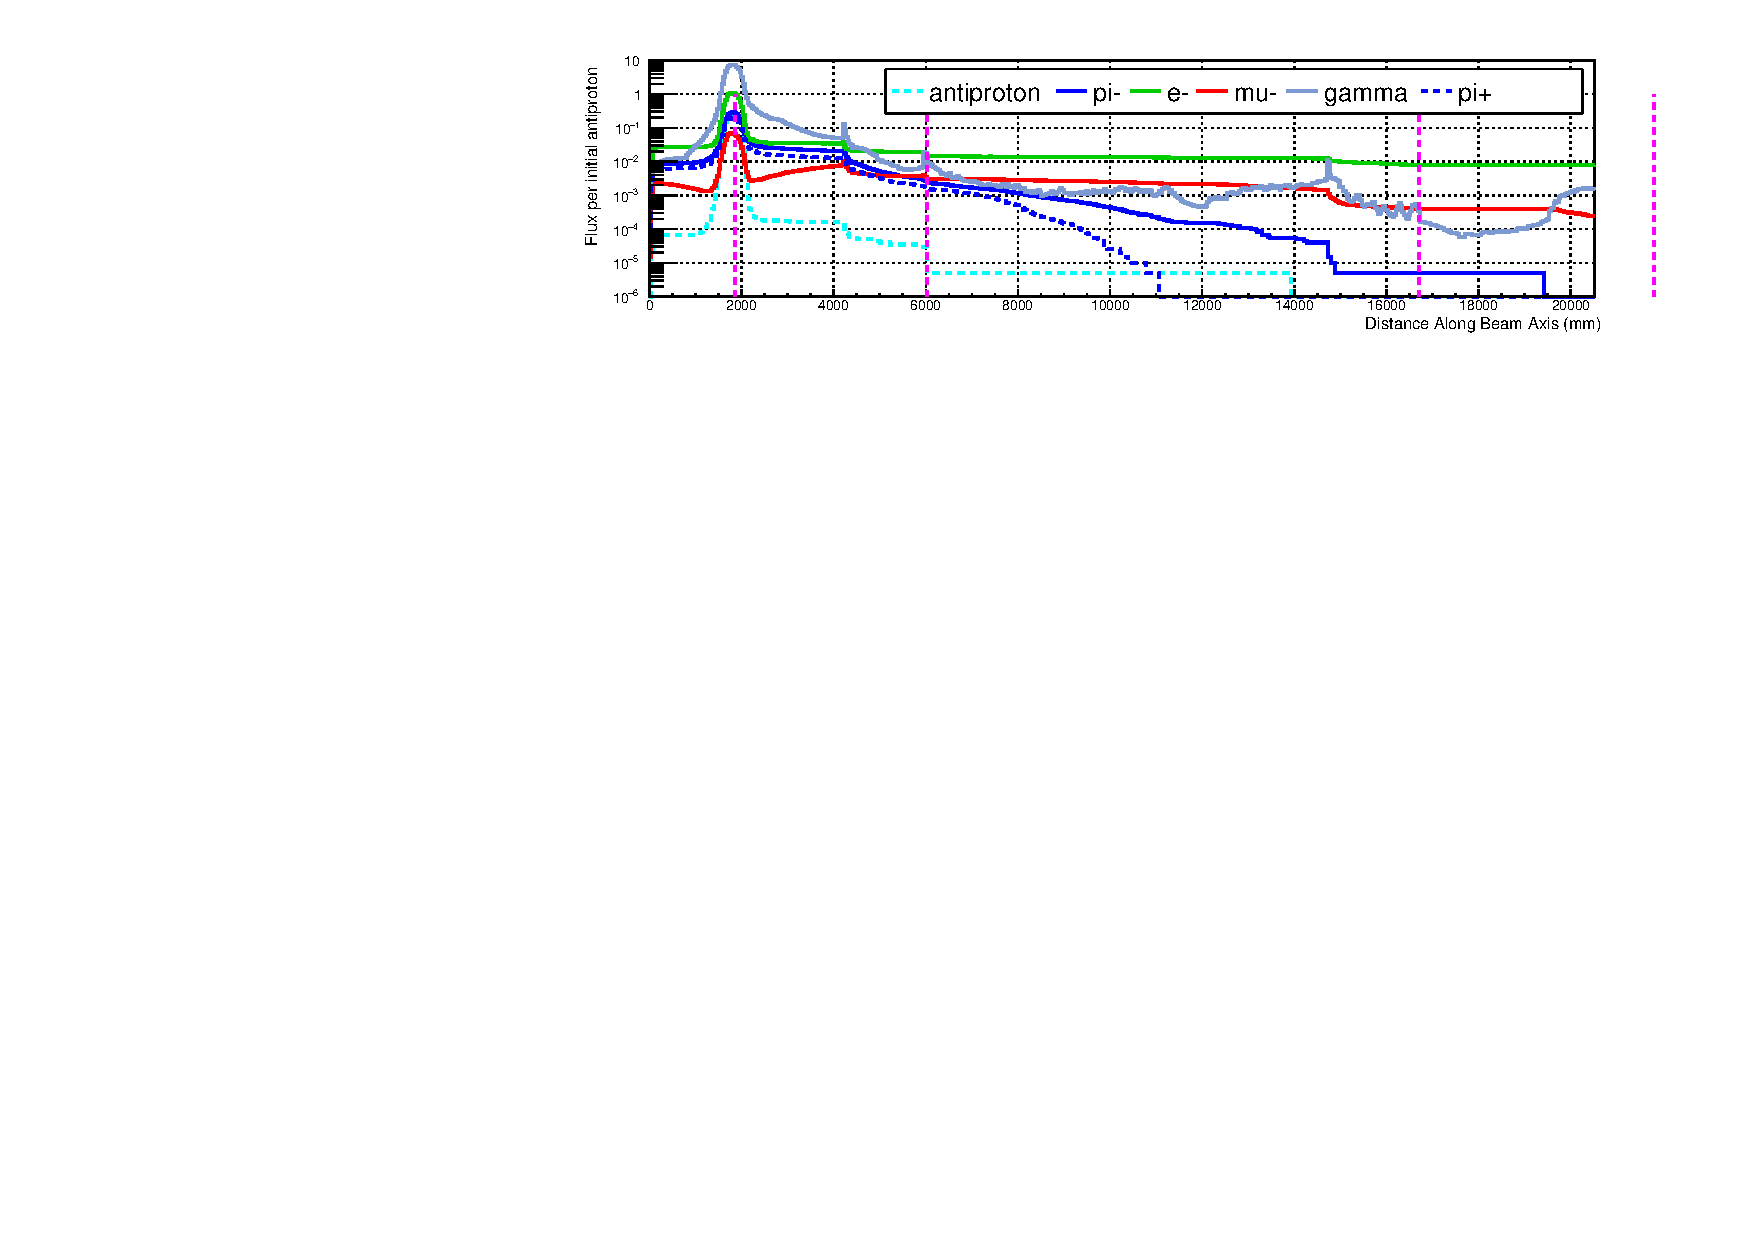
\includegraphics[width=1\textwidth,trim=0.7cm 0 1.9cm 0.2cm,clip]{figs/backgrounds/Antiproton_flux_59.pdf}}\\
%\subfloat[][\figlabel{bg:antiprotons:sim:fluxes:97}Production between 97 and 119\degree]{
%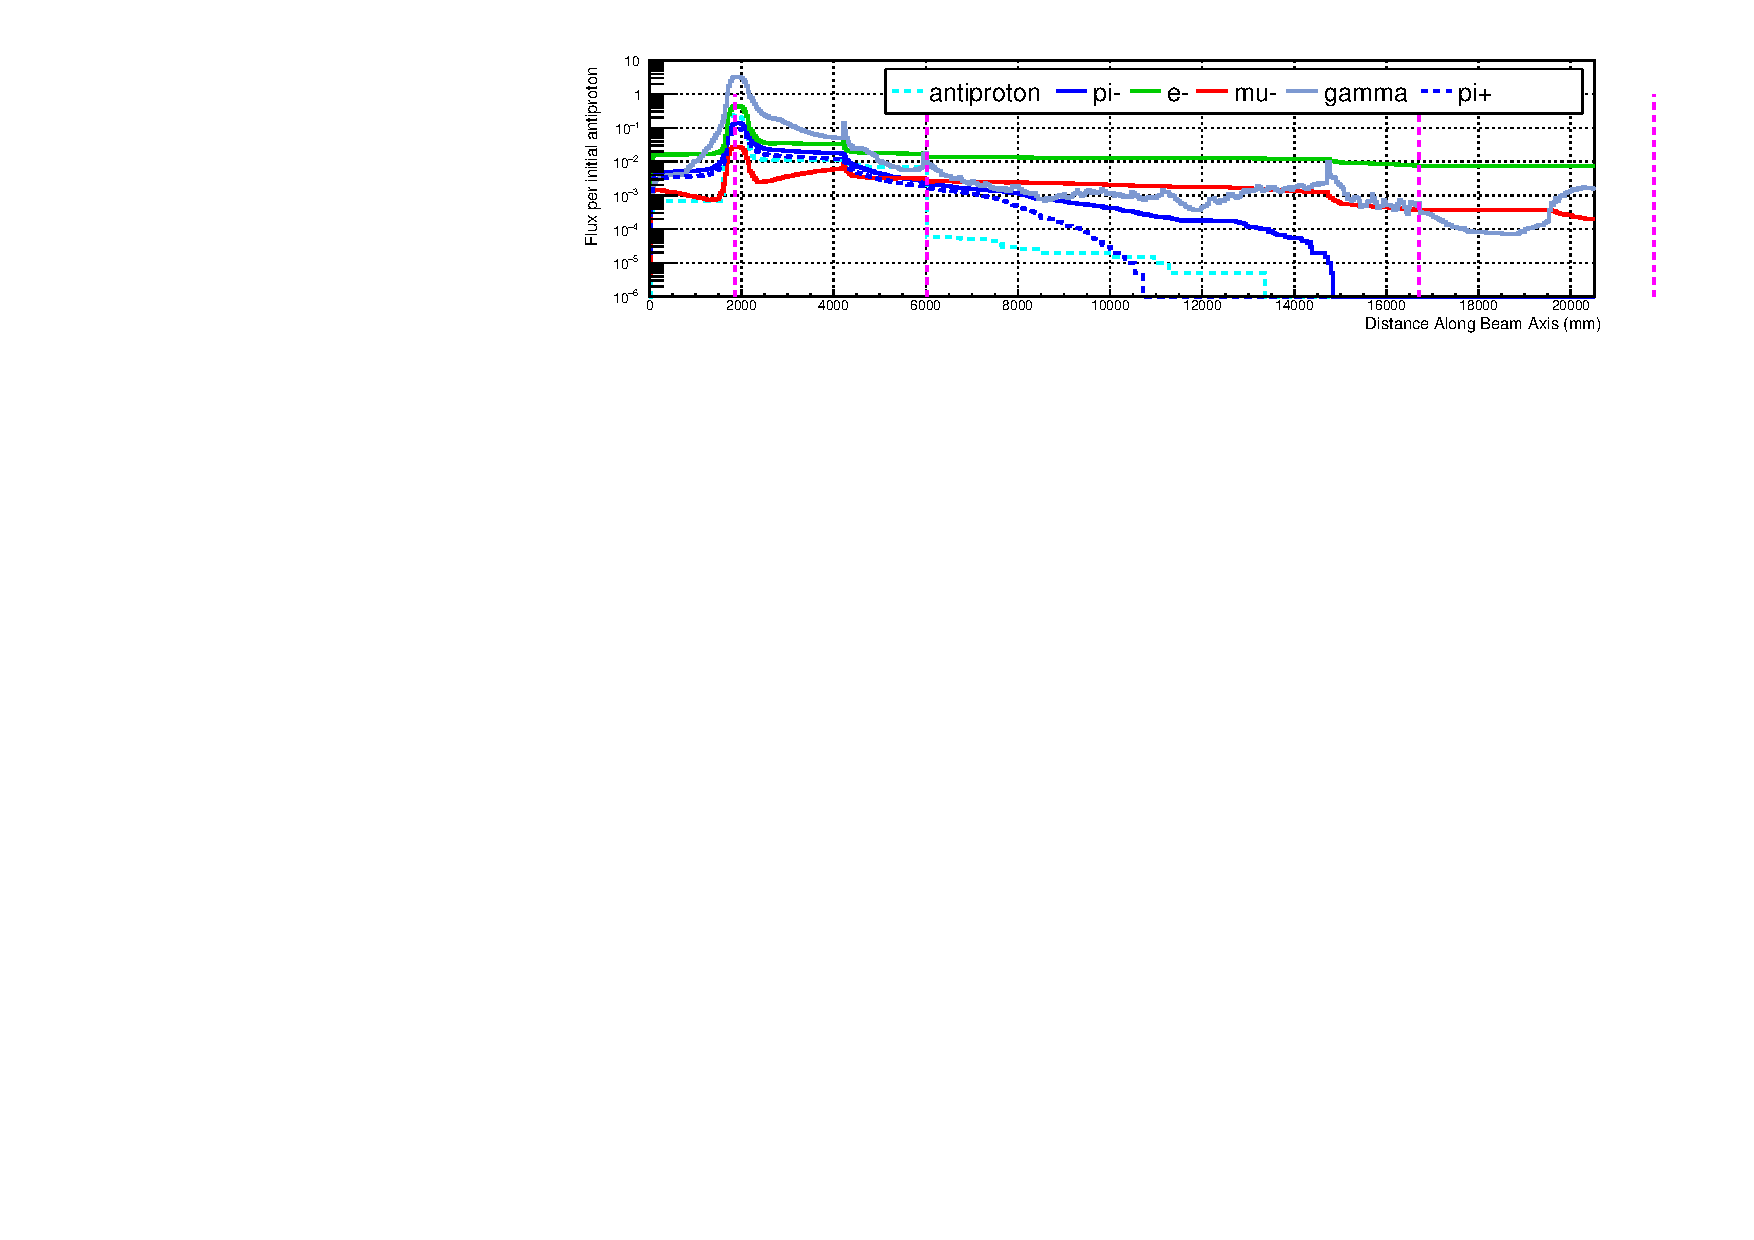
\includegraphics[width=1\textwidth,trim=0.7cm 0 1.9cm 0.2cm,clip]{figs/backgrounds/Antiproton_flux_97.pdf}}\\
%\subfloat[][\figlabel{bg:antiprotons:sim:fluxes:119}Production between 119 and 180\degree]{
%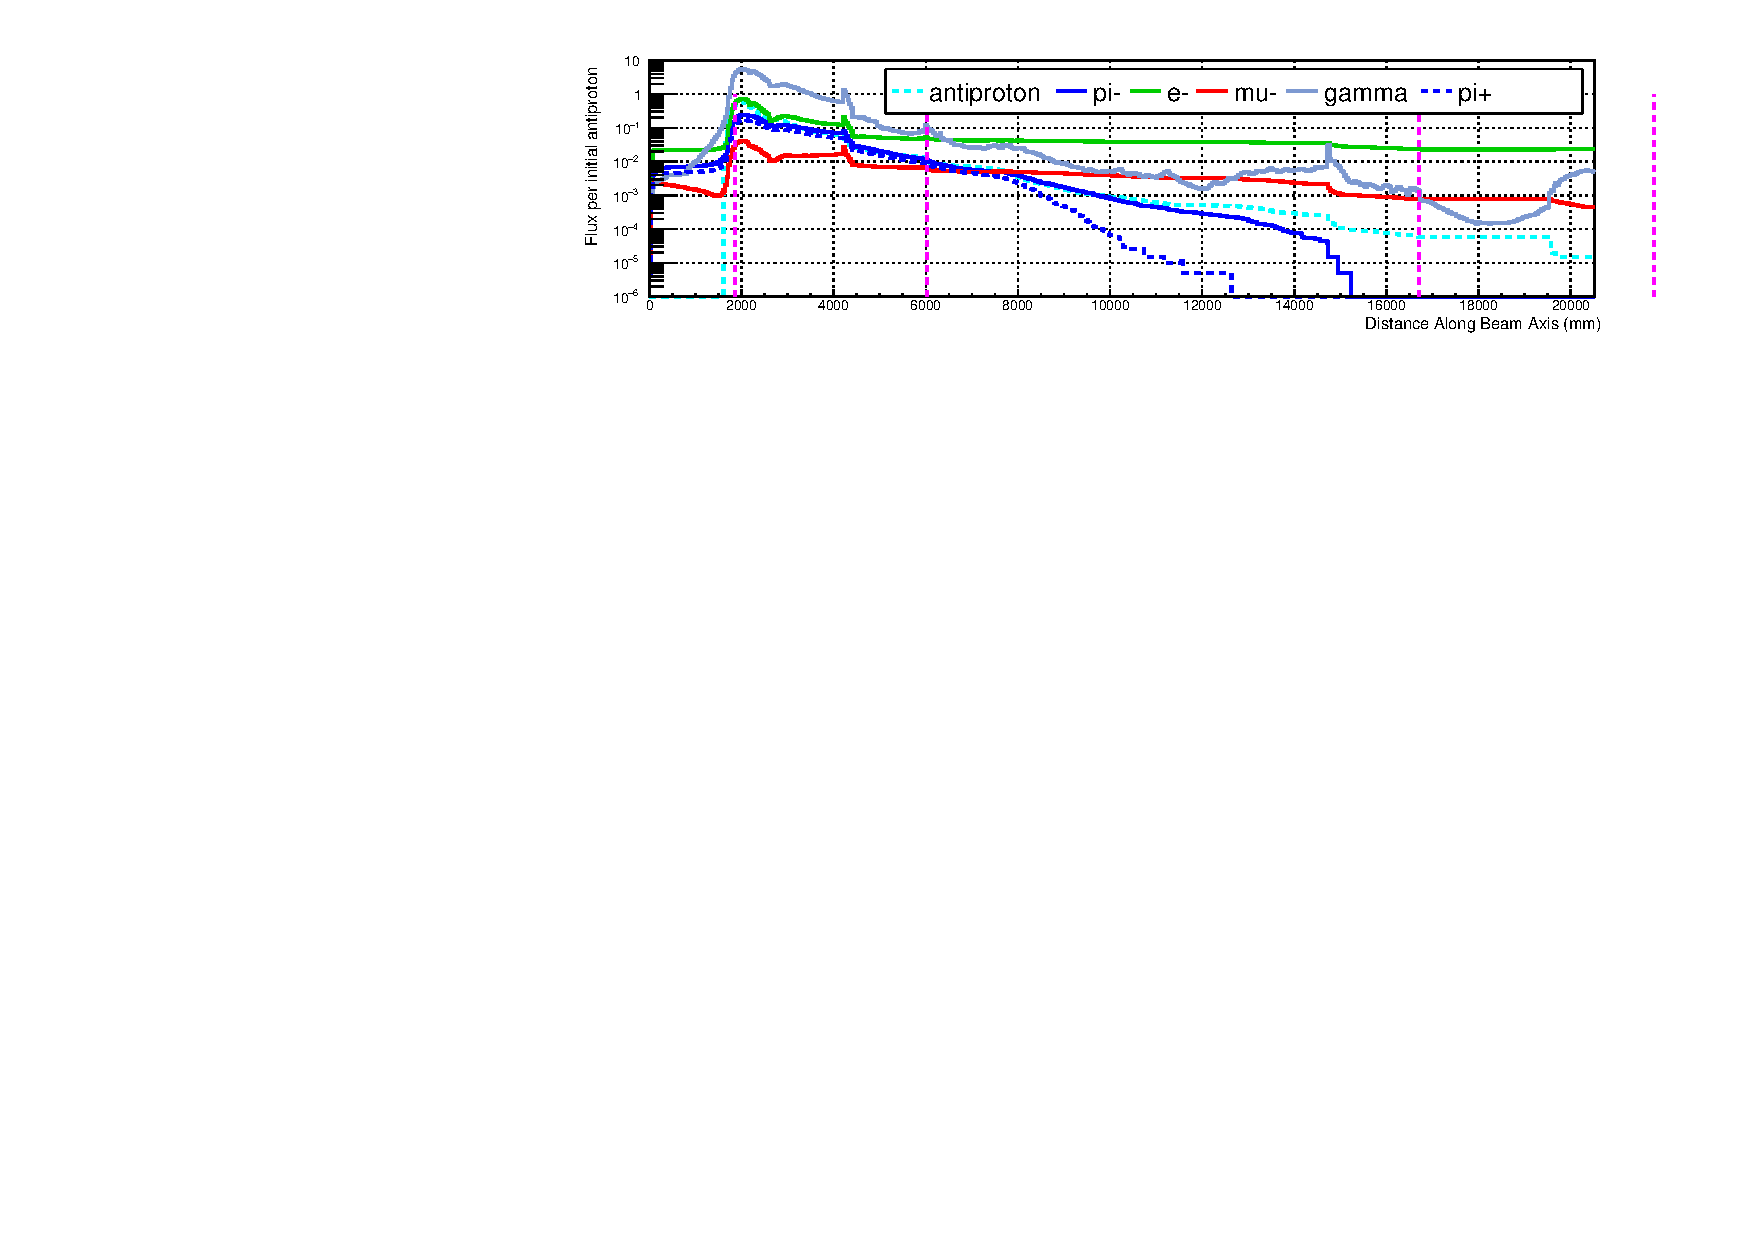
\includegraphics[width=1\textwidth,trim=0.7cm 0 1.9cm 0.2cm,clip]{figs/backgrounds/Antiproton_flux_119.pdf}}
%\caption{\figlabel{bg:antiprotons:sim:fluxes}
%The surivival probability of antiprotons and their secondaries per antiproton produced in the target as a function of distance along the beamline.
%From left to right the vertical magenta lines indicate the production target, Torus1 entrance, and the Torus2 exit.
%}
%\end{figure}
%}

\newcommand{\FigAntiprotonSimPiMom}{
\begin{figure}[tb]
\centering 
\includegraphics[width=0.9\textwidth,trim=2.0cm 0 0 0,clip]{figs/backgrounds/Antiproton_pion_momentum.pdf}
\caption{\figlabel{bg:antiprotons:sim:piMom}
Momentum of pions passing the exit of Torus1 (90\degree around the bent muon beam transport solenoid) compared to pions in the main muon beam (which is arbitrarily normalised).
}
\end{figure}
}

\newcommand{\HeaderPi}[1]{\multicolumn{1}{#1}{Torus1 $\pi^-$}}
\newcommand{\HeaderPBar}[1]{\multicolumn{1}{#1}{$\bar{p}$ Stop}}
%\newcommand{\TabAntiprotonResults}{
%\begin{table}[tb]
%\centering
%\begin{tabular}{a|SS|SS|SS|}
%\multicolumn{1}{c|}{Region} & \multicolumn{2}{c|}{Observed Events} & \multicolumn{2}{c|}{Weighted Mean per $\bar{p}$}& \multicolumn{2}{c}{Rate per \ac{POT}}  \\
%\multicolumn{1}{c|}{}       & \HeaderPi{r}    & \HeaderPBar{r|}    & \HeaderPi{r}      & \HeaderPBar{r|}      &\HeaderPi{r}     & \HeaderPBar{r}                  \\
%\hline
%   0-59\degree &50&0&2.5e-4&& \\
%  59-97\degree &31&0&1.6e-4&& \\
% 97-119\degree &36&0&1.8e-4&& \\
%119-180\degree &64&9&3.2e-4&& \\
%\hline
%\multicolumn{1}{c|}{Total} & & & & & \\
%\hline
%\end{tabular}
%\caption{\tablabel{bg:antiprotons:results}
%Results of the antiproton simulation.
%`Torus1 $\pi^-$' are the pions that pass the exit of Torus1, which is 90\degree round the muon beamline.
%`$\bar{p}$ Stop' refers to the number of antiprotons that stop in the muon Stopping Target.
%The weighted mean is the sum of the observed events weighted by the production probability given the initial antiproton direction, divided by the total number of input antiprotons.
%Finally the Rate per \ac{POT} is weighted mean scaled by the number of antiprotons produced for this region per POT (last column of \tab{bg:antiprotons:regions}).
%}
%\end{table}
%}

%\newcommand{\TabAntiprotonResultsPiSecond}{
%\begin{table}[tb]
%\centering
%\begin{tabular}{a|SSS}
%\multicolumn{1}{c|}{Region} & \multicolumn{1}{c}{Observed Events} & \multicolumn{1}{c}{Weighted Mean per $\bar{p}$}& \multicolumn{1}{c}{Rate per \ac{POT}}  \\
%\hline
%   0-59\degree &50&2.5e-4&& \\
%  59-97\degree &31&1.6e-4&& \\
% 97-119\degree &36&1.8e-4&& \\
%119-180\degree &64&3.2e-4&& \\
%\hline
%\multicolumn{1}{c|}{Total} & & & & & \\
%\hline
%\end{tabular}
%\caption{\tablabel{bg:antiprotons:results}
%Results of the antiproton simulation.
%`Torus1 $\pi^-$' are the pions that pass the exit of Torus1, which is 90\degree round the muon beamline.
%`$\bar{p}$ Stop' refers to the number of antiprotons that stop in the muon Stopping Target.
%The weighted mean is the sum of the observed events weighted by the production probability given the initial antiproton direction, divided by the total number of input antiprotons.
%Finally the Rate per \ac{POT} is weighted mean scaled by the number of antiprotons produced for this region per POT (last column of \tab{bg:antiprotons:regions}).
%}
%\end{table}
%}

%\newcommand{\TabAntiprotonResultsTrans}{
%\begin{table}[p]
%\centering
%\begin{tabular}{a|SSS|SSS|S|}
% &\multicolumn{3|}{c}{Raw count} &\multicolumn{3|}{c}{Weighted Probability} & \\
% &\multicolumn{1}{p{0.6cm}}{Entr.}&\multicolumn{1}{p{0.6cm}}{Mid.}&\multicolumn{1}{p{0.6cm}|}{Target}&\multicolumn{1}{p{0.6cm}}{Entr.}&\multicolumn{1}{p{0.6cm}}{Mid.}&\multicolumn{1}{p{0.6cm}}{Target}&\multicolumn{1}{p{0.6cm}}{$P(\textrm{Target}|\textrm{Entr.}$}\\
%\hline
%\multicolumn{1}{l}{Pions} & \multicolumn{7}{p{6cm}}{}\\
%   0-59\degree    & 16943  & 1452  & 1  & 5.77E-06 & 5.10E-07 & 9.98E-11 & 1.73E-05 \\ 
%   59-97\degree   & 87230  & 7157  & 18 & 4.64E-09 & 4.06E-10 & 2.99E-13 & 6.45E-05 \\ 
%   97-119\degree  & 157385 & 13041 & 25 & 4.10E-14 & 3.59E-15 & 5.02E-18 & 1.22E-04 \\ 
%   119-180\degree & 222486 & 12997 & 30 & 1.25E-17 & 9.59E-19 & 1.91E-21 & 1.53E-04 \\ 
%\hline
%\multicolumn{1}{l}{Antiprotons} & \multicolumn{7}{p{6cm}}{}\\
%0-59\degree    & 7      & 3     & 0    & 1.40E-09 & 5.14E-11 & 3.23E-12                  &          \\ 
%59-97\degree   & 270    & 58    & 8    & 1.70E-12 & 4.81E-13 & 1.16E-14                  & 2.41E-02 \\ 
%97-119\degree  & 2907   & 830   & 114  & 1.10E-16 & 3.31E-17 & 5.17E-19                  & 1.56E-02 \\ 
%119-180\degree & 278105 & 20787 & 2237 & 2.27E-19 & 5.20E-20 & 7.74E-21                  & 1.49E-01 \\ 
%               &        &       &      &          &          & \multicolumn{1}{c}{Mean=} & 6.29E-02 \\ 
%%\hline
%\end{tabular}
%\end{table}
%}

\newcommand{\TabAntiprotonResultsPiSecond}{%
\begin{table}[p]%
\sisetup{table-number-alignment=right, table-format=2.2e2}%
\centering%
%\begin{adjustwidth}{-0.7cm}{}%
\begin{tabular}{lr|S!{\VRule}S!{\VRule}S!{\VRule}S|}%
\multicolumn{2}{c|}{\multirow{2}{3cm}{Rates for Secondary $\pi^-$}} & \multicolumn{4}{c|}{Secondary $\pi^-$ from Angular Region for Antiproton Production} \\ 
                              &  & \multicolumn{1}{a!{\VRule}}{0-59\degree} & \multicolumn{1}{a!{\VRule}}{59-97\degree} & \multicolumn{1}{a!{\VRule}}{97-119\degree} & \multicolumn{1}{a|}{119-180\degree} \\ 
\hline
\multirow{3}{1.6cm}{Raw Counts} & Torus1 & \multicolumn{1}{r!{\VRule}}{16943} & \multicolumn{1}{r!{\VRule}}{87230} & \multicolumn{1}{r!{\VRule}}{157385} & \multicolumn{1}{r|}{222486} \\ 
                               %& TS3    & \multicolumn{1}{r!{\VRule}}{1452}  & \multicolumn{1}{r!{\VRule}}{7157}  & \multicolumn{1}{r!{\VRule}}{13041}  & \multicolumn{1}{r|}{12997}  \\ 
                                & Torus2 & \multicolumn{1}{r!{\VRule}}{208}   & \multicolumn{1}{r!{\VRule}}{1106}  & \multicolumn{1}{r!{\VRule}}{1995}   & \multicolumn{1}{r|}{1847}   \\ 
                                & Target & \multicolumn{1}{r!{\VRule}}{1}     & \multicolumn{1}{r!{\VRule}}{18}    & \multicolumn{1}{r!{\VRule}}{25}     & \multicolumn{1}{r|}{30}     \\ 
\hline
\multirow{3}{1.6cm}{Weighted Sum} & Torus1  & 5.77e-6  & 4.64E-09 & 4.10E-14 & 1.25E-17 \\ 
                                  %& TS3    & 5.10e-7  & 4.06E-10 & 3.59E-15 & 9.59E-19 \\ 
                                  & Torus2  & 8.59e-8  & 5.93E-11 & 5.79E-16 & 1.23E-19 \\ 
                                  & Target  & 9.98e-11 & 2.99E-13 & 5.02E-18 & 1.91E-21 \\ 
\hline
\multicolumn{2}{r|}{$P(\textrm{Target}|\textrm{Torus2})$}  & 0.039 & 0.040 &  0.022 & 0.017 \\
\hline
\end{tabular}%
%\end{adjustwidth}%
\caption{\tablabel{bg:antiprotons:sim:pi}%
The simulated number of secondary pions from antiprotons observed at key points along the beamline.
The raw counts are the total observed events from the simulation of 80M antiprotons for each of the four angular regions.
The weighted sum then shows the weighted sum over every particle passing the point, where the weight is determined as described by equation~\eq{bg:antiprotons:factorisation}.
The final row, $P(\textrm{Target}|\textrm{Torus2 Coll.})$, gives the survival probability for a pion to reach the target, given that it passed the Torus1 Entrance, \ie it is the ratio between the Target and Torus1 Entrance rates.
}\end{table}\xspace}

\newcommand{\TabAntiprotonResultsAntip}{
\begin{table}[p]%
\sisetup{table-number-alignment=right, table-format=2.2e2}%
%\begin{adjustwidth}{-0.7cm}{}%
\begin{tabular}{lr|S!{\VRule}S!{\VRule}S!{\VRule}S|}%
\multicolumn{2}{c|}{\multirow{2}{3cm}{Rates for $\bar{p}$ Transport}} & \multicolumn{4}{c|}{Angular Region for Antiproton Production} \\ 
                              &  & \multicolumn{1}{a!{\VRule}}{0-59\degree} & \multicolumn{1}{a!{\VRule}}{59-97\degree} & \multicolumn{1}{a!{\VRule}}{97-119\degree} & \multicolumn{1}{a|}{119-180\degree} \\ 
\hline
\multirow{3}{1.6cm}{Raw Counts} & Torus1 &\multicolumn{1}{r!{\VRule}}{7} & \multicolumn{1}{r!{\VRule}}{270} & \multicolumn{1}{r!{\VRule}}{2907} & \multicolumn{1}{r|}{278105} \\ 
                                %& TS3                 & \multicolumn{1}{r!{\VRule}}{3} & \multicolumn{1}{r!{\VRule}}{58 } & \multicolumn{1}{r!{\VRule}}{830 } & \multicolumn{1}{r|}{20787 } \\ 
                                & Torus2 & \multicolumn{1}{r!{\VRule}}{1} & \multicolumn{1}{r!{\VRule}}{39 } & \multicolumn{1}{r!{\VRule}}{431 } & \multicolumn{1}{r|}{9024  } \\ 
                                & Target &\multicolumn{1}{r!{\VRule}}{0} & \multicolumn{1}{r!{\VRule}}{8  } & \multicolumn{1}{r!{\VRule}}{114 } & \multicolumn{1}{r|}{2237  } \\ 
\hline
\multirow{3}{1.6cm}{Weighted Sum} & Torus1 & 1.40E-09 & 1.70E-12&1.10E-16 & 2.27E-19\\ 
                                  %& TS3                 & 5.14E-11 & 4.81E-13&3.31E-17 & 5.20E-20\\ 
                                  & Torus2 & 1.62E-14 & 5.15E-14&1.54E-17 & 2.63E-20\\ 
                                  & Target & {*}3.65E-15 & 1.16E-14&5.17E-19 & 7.74E-21\\ 
\hline                                                           
\multicolumn{2}{r|}{$P(\textrm{Target}|\textrm{Torus2})$} &{*}0.225& 0.225  & 0.034  & 0.295\\
\hline
\end{tabular}%
%\end{adjustwidth}%
\caption{\tablabel{bg:antiprotons:sim:antip}%
Antiproton stopping rates and fluxes at key points.%
Since no antiprotons were seen stopping for the angular region from 0 to 59\degree, the value for the final two entries in that column --- indicated with an asterisk (*) ---  are obtained by multiplying the antiproton rate expected at the Torus2 collimator with the median collimator acceptance from the other three angular regions.%
%The mean acceptance of the Torus2 collimator is 0.185.%
For each of the angular regions, 80 million antiprotons were simulated.%
}\end{table}\xspace}

%\newcommand{\TabAntiprotonFactors}{
%\begin{table}[tb]
%\centering
%        \begin{tabular}{llm{0.5\textwidth}}
%	\hline
%        Parameter & \multicolumn{1}{l}{Value} & Description \\
%	\hline
%        $R_{\pi/p}$                & \VarPiStopsPerPOT & Pion stopping rate per \ac{POT}  \\ 
%        $\mathcal{B}_\textrm{RPC}$ & \num{2.27e-2} & Branching ratio of \ac{RPC} \\ 
%	$f_{e,\textrm{RPC}}$           & \VarDetectedEsPerRPC & Probability of an RPC photon producing signal-like electrons in the detector \\ 
%	$A_\textrm{time}$              & \VarRPCTimingEfficiency & Acceptance of timing window to secondary electrons from RPC \\ 
%        $\epsilon_\textrm{extinction}$ & \VarExtinctionFactor[2] &  Extinction factor\\ 
%	\hline
%\end{tabular}
%\caption{\tablabel{bg:antiprotons:factors}
%Parameters and their values in the determination of the \ac{RPC} background rate.
%}
%\end{table}
%}

\newcommand{\TabAntiprotonEstimates}{
\begin{table}[tbp]
\sisetup{table-number-alignment=right, table-format=2.2e3, table-comparator=true}
%\begin{adjustwidth}{-0.9cm}{}
\begin{tabular}{la|SS|SS|}
            &         & \multicolumn{2}{c|}{Stopping Rates} & \multicolumn{2}{c|}{Background Rate per POT} \\ 
            &         & {Unweighted} & {Weighted} & {No Timing} & {With Timing}  \\
\hline
\multirow{4}{*}{$\bar{p}$} & 0-59    & <6.58E-13              & <3.65E-15   & 1.69E-21      & 8.66E-22    \\ 
            & 59-97   & 4.17E-16              & 1.16E-14   & 5.36E-21      & 2.75E-21    \\ 
            & 97-119  & 2.48E-18              & 5.17E-19   & 2.39E-25      & 1.23E-25    \\ 
            & 119-180 & 1.60E-17              & 7.74E-21   & 3.58E-27      & 1.84E-27    \\ 
\hline
\multirow{4}{*}{$\pi^-$}       & 0-59    & 6.58E-13              & 9.98E-11   & 2.95E-17      & 1.62E-29    \\ 
            & 59-97   & 9.38E-16              & 2.99E-13   & 8.86E-20      & 4.86E-32    \\ 
            & 97-119  & 5.44E-19              & 5.02E-18   & 1.49E-24      & 8.15E-37    \\ 
            & 119-180 & 2.14E-19              & 1.91E-21   & 5.65E-28      & 3.10E-40    \\ 
\hline
 \multicolumn{4}{r|}{Sum (per POT)}                         & 2.96E-17      & 3.62e-21    \\ 
\hline
\end{tabular}
%\end{adjustwidth}
\caption{\tablabel{bg:antiprotons:estimates}
Final estimated background rates.
See text for column definitions.
}
\end{table}\xspace}

\newcommand{\FigBgBeamMomVsTime}{
\begin{figure}[t]
\centering 
\subfloat[][\figlabel{bg:beam:MomVsTime:strawTrk}$e^-$ at the Straw Tracker]{
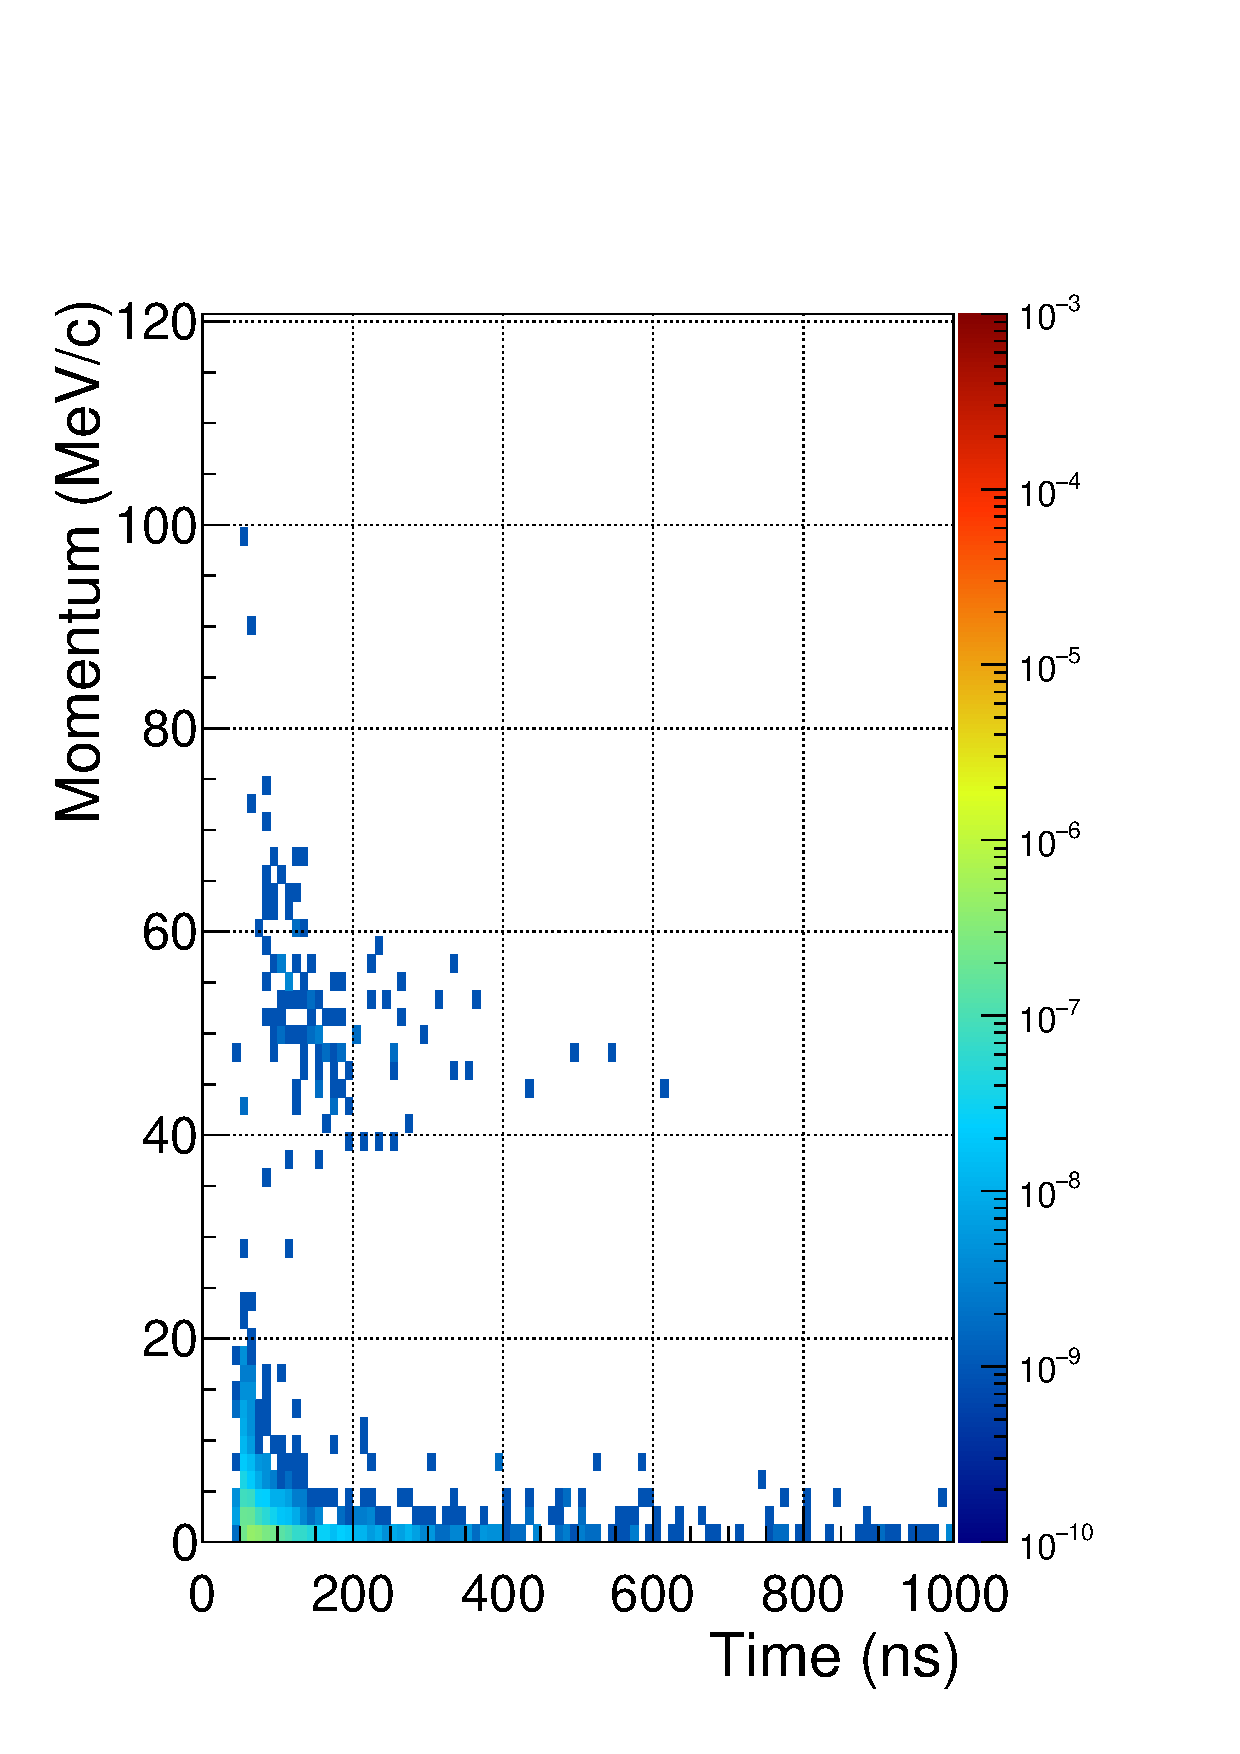
\includegraphics[width=0.45\textwidth,trim=0 0 0 1.7cm,clip]{figs/backgrounds/Beam_TimeVsMomentum_StrawTkt.pdf}}
\subfloat[][\figlabel{bg:beam:MomVsTime:stopTgt}$e^-$ after the Beam Blocker]{
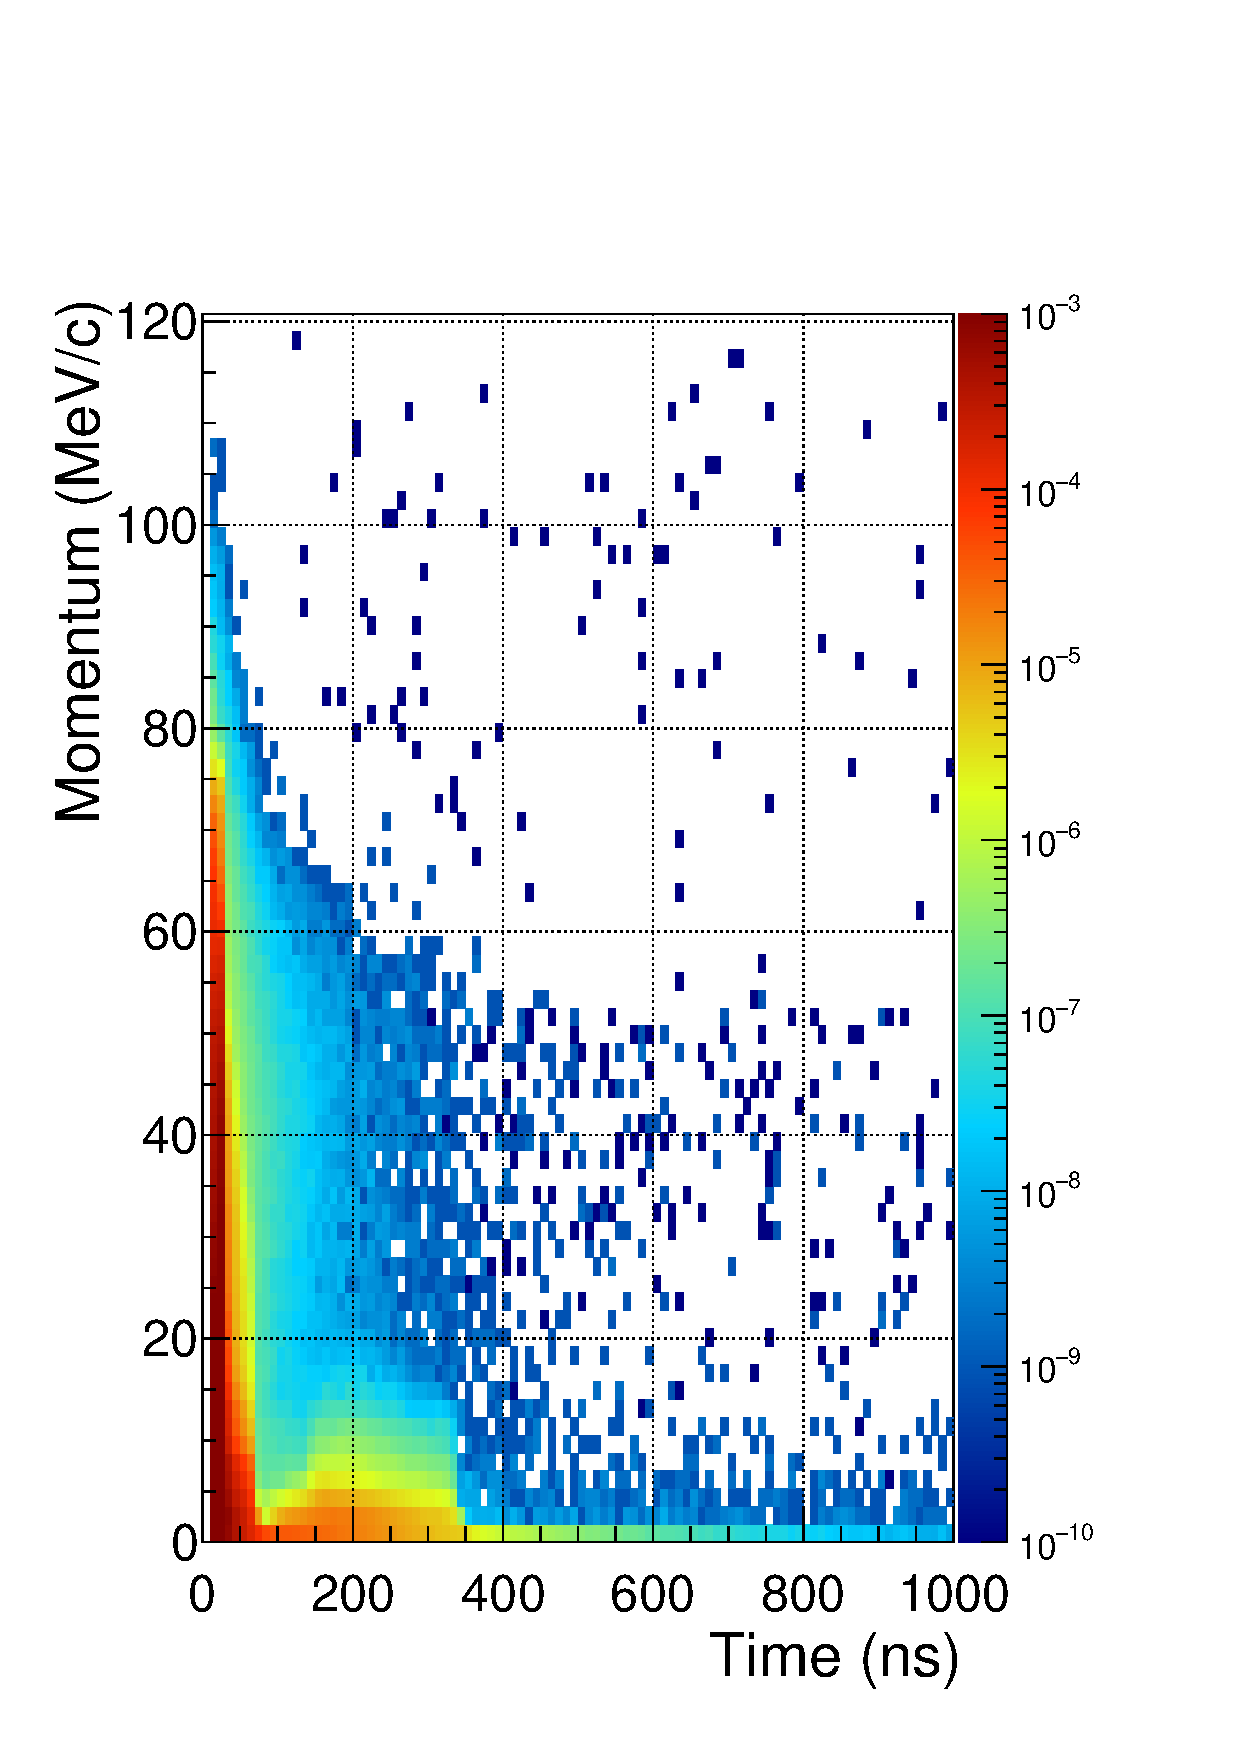
\includegraphics[width=0.45\textwidth,trim=0 0 0 1.7cm,clip]{figs/backgrounds/Beam_TimeVsMomentum_StopTgt.pdf}}
\caption{\figlabel{bg:beam:MomVsTime}
The timing and momentum of electrons detected at the straw tracker and passing a plane immediately after the beam blocker.
}
\end{figure}
}

\newcommand{\FigBgBeamExtrapolate}{
\begin{figure}[t]
\centering 
\subfloat[][\figlabel{bg:beam:acceptance:momentum}Momentum of electrons]{
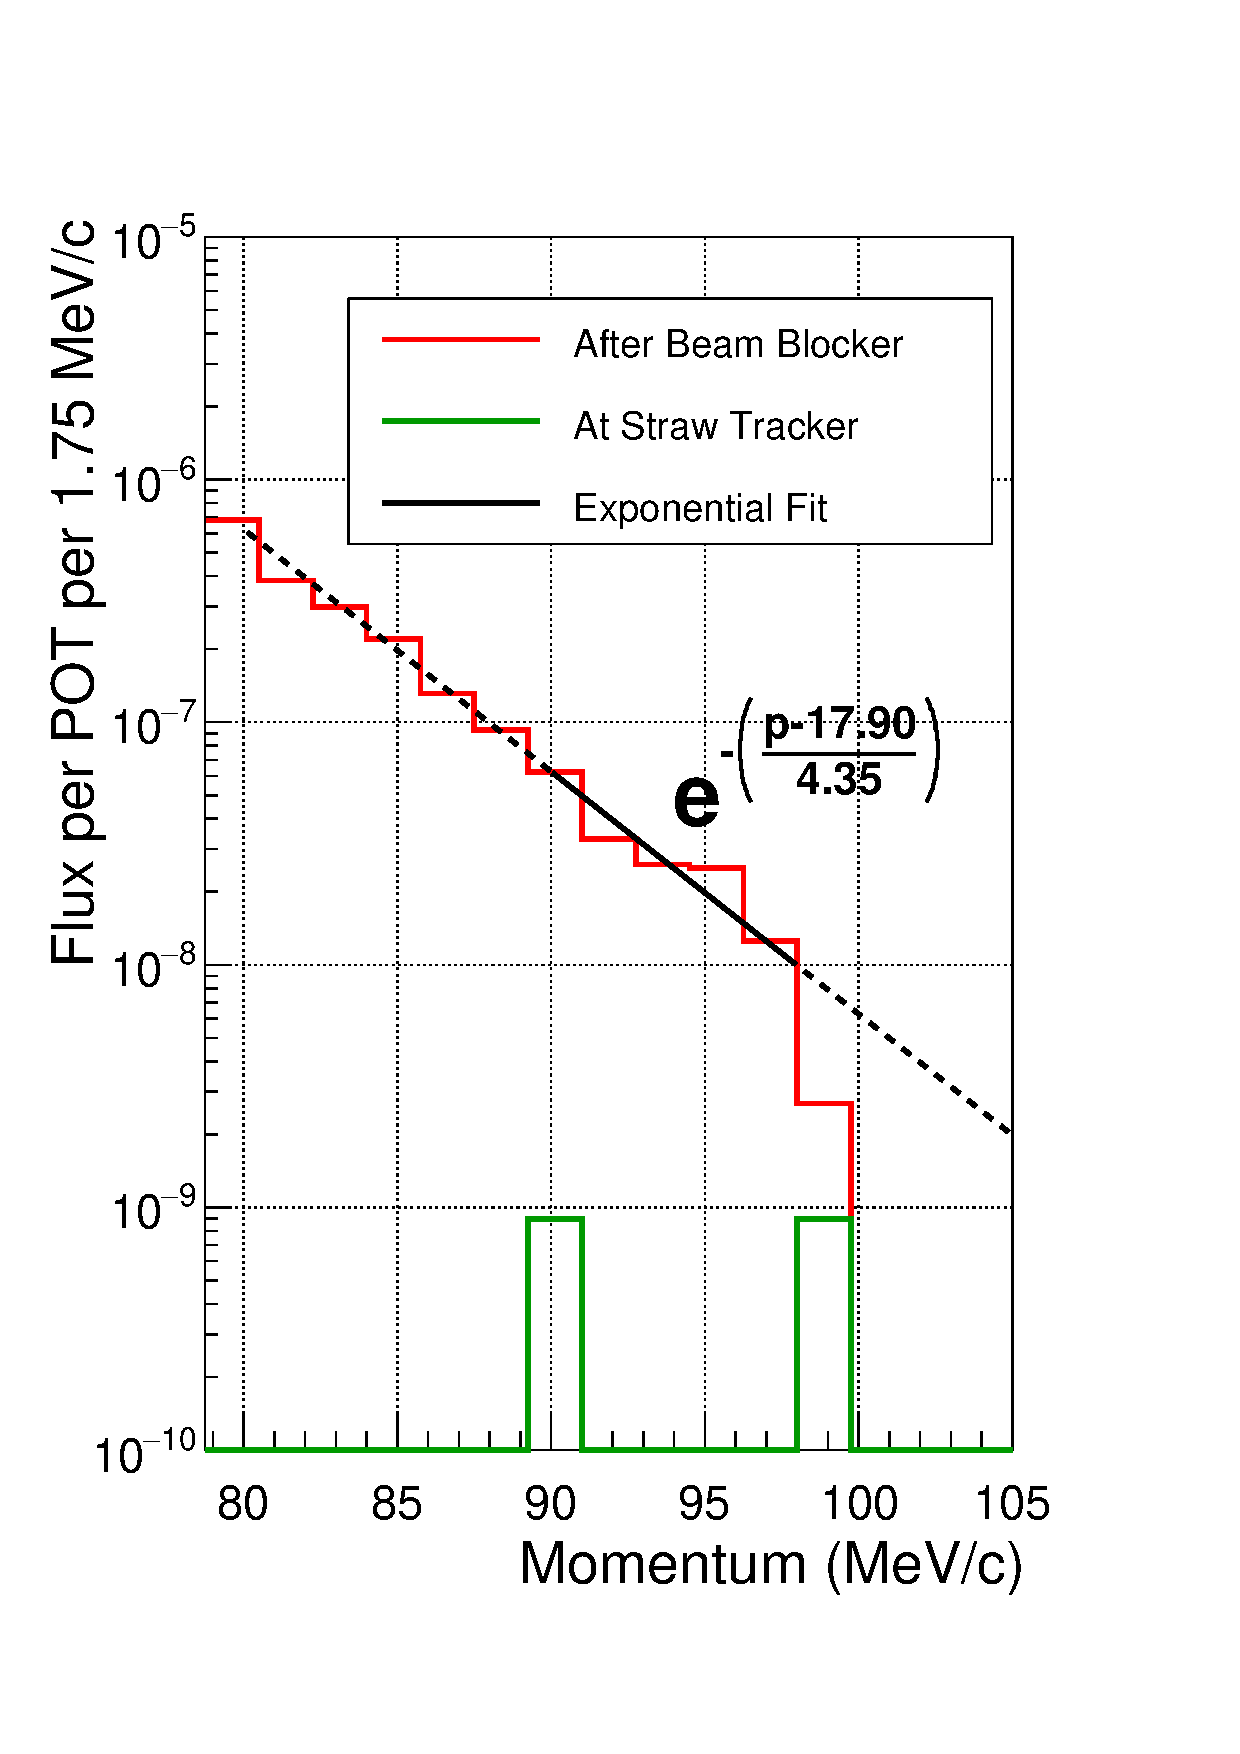
\includegraphics[width=0.49\textwidth,trim=0 1.5cm 0 0.7cm,clip]{figs/backgrounds/Beam_Acceptance_momentum.pdf}}
\subfloat[][\figlabel{bg:beam:acceptance:time}Time of high-$p$ electrons]{
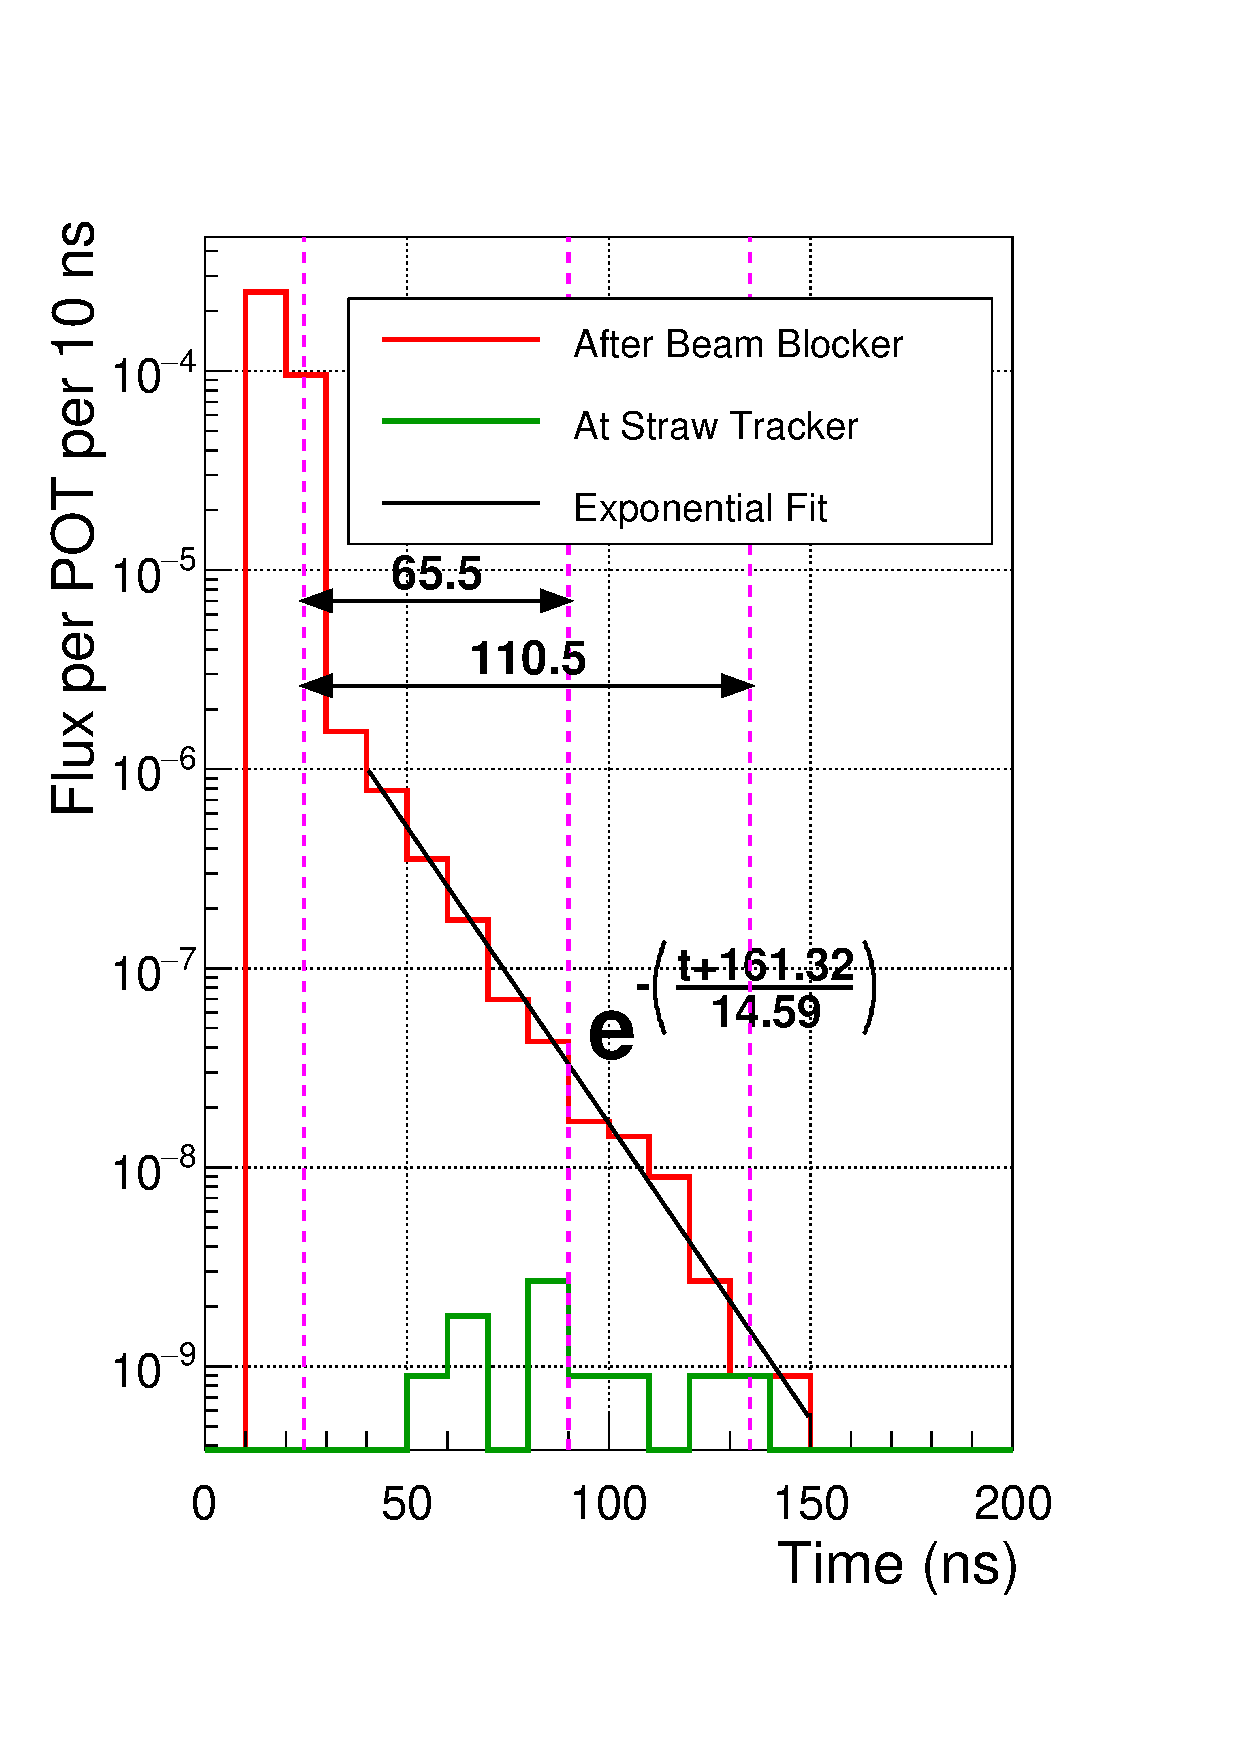
\includegraphics[width=0.49\textwidth,trim=0 1.5cm 0 0.7cm,clip]{figs/backgrounds/Beam_Acceptance_time.pdf}}
\caption{\figlabel{bg:beam:acceptance}
Projections of the momentum and arrival time of electrons.
\protect\subref{fig:bg:beam:acceptance:momentum} shows the momentum for electrons that arrive at any time, 
whereas \protect\subref{fig:bg:beam:acceptance:time} only shows the arrival time for electrons with momentum above 65~MeV/c.
Magenta lines in \protect\subref{fig:bg:beam:acceptance:time} indicate the mean arrival time after the beam blocker and the mean and maximum arrival time
at the straw tracker.
The black line is an exponential fit to the momentum and time of electrons after the beam blocker, with the equation and constants shown next to the fit.
%Below this momentum, electrons from muon decay-in-orbit dominate the timing.
}
\end{figure}
}

\newcommand{\TabBackgroundFinalVals}{
\begin{table}
\centering
%	\renewcommand{\arraystretch}{1} % Default value: 1
\begin{tabular}{ll|SSS|S}
Type & Source & \multicolumn{3}{c|}{Background Rate}       & {Total Events} \\ 
     &        & {per Stopping $\mu^-$}  & {per POT}  &  {per \si{s}} &              \\ 
\hline
\hline
Total & & & & & \\
\hline
\end{tabular}
\caption{ \tablabel{bg:summary}%
Final predicted background rates and events.
Assumes....
}
\end{table}%
}

